%%% DOCUMENTCLASS 
%%%-------------------------------------------------------------------------------

\documentclass[
a4paper, % Stock and paper size.
11pt, % Type size.
% article,
%oneside, 
onecolumn, % Only one column of text on a page.
%openright, % Each chapter will start on a recto page.
%openleft, % Each chapter will start on a verso page.
openany, % A chapter may start on either a recto or verso page.
%notitlepage % prvni stranku si udelam sama
oldfontcommands,
]{memoir}

%%% PACKAGES 
%%%------------------------------------------------------------------------------

\usepackage[utf8]{inputenc} % If utf8 encoding
% \usepackage[lantin1]{inputenc} % If not utf8 encoding, then this is probably the way to go
\usepackage[T1]{fontenc}    %
\usepackage[english]{babel} % English please
\usepackage[final,letterspace=-30]{microtype} % Less badboxes
% \usepackage{kpfonts} %Font
\usepackage{amsmath,amssymb,mathtools} % Math
% \usepackage{tikz} % Figures
\usepackage[final]{pdfpages} % insert PDF
\usepackage{epstopdf}
\usepackage{graphicx} % Include figures
\usepackage{aas_macros}
%\usepackage[round]{natbib}
\usepackage{dcolumn}% Align table columns on decimal point

\usepackage{amsmath,amssymb,amsthm}
\usepackage{mathptmx}  %% volne dostupny font Adobe Times Roman
\usepackage{siunitx} % align tabularx
\usepackage{longtable}
\usepackage{dcolumn}% Align table columns on decimal point
\usepackage{bm}

\usepackage[square,numbers]{natbib} %nastavuje bibtex
\bibliographystyle{plainnat}


%%% sci rep usepackage
\usepackage{calrsfs}
%\usepackage{physics}
%\usepackage{siunitx}
%\usepackage{breqn}
\usepackage{todonotes}
%%% end sci rep usepackage

\newsavebox{\foobox}
\newcommand{\slantbox}[2][0]{\mbox{%
		\sbox{\foobox}{#2}%
		\hskip\wd\foobox
		\pdfsave
		\pdfsetmatrix{1 0 #1 1}%
		\llap{\usebox{\foobox}}%
		\pdfrestore
}}
\newcommand\unslant[2][-.20]{\slantbox[#1]{$#2$}}


\newcommand\ualpha{\unslant\alpha}
\newcommand\sualpha{\scriptsize\unslant\alpha\kern-0.075em}
\newcommand\udelta{\unslant\delta}
\newcommand\upi{\unslant\pi}
\newcommand\umu{\unslant\mu}




%%% PAGE LAYOUT 
%%%------------------------------------------------------------------------------

%\setlrmarginsandblock{0.18\paperwidth}{*}{1} % Left and right margin % original: 0.15
%\setlrmarginsandblock{4.35cm}{3.35cm}{*} % rozlozeni na tisk -- v knihtisku orezou 11mm zleva a 1mm ze zbyvajicich stran
\setlrmarginsandblock{3.7cm}{2.7cm}{*} % rozlozeni na tisk -- v knihtisku orezou 11mm zleva a 1mm ze zbyvajicich stran
\setulmarginsandblock{0.2\paperwidth}{*}{1}  % Upper and lower margin
\checkandfixthelayout % obrátí okraje, když chceme oboustrannou sazbu, musí sudé stránky převrátit, při jednom stranné sazbě předchozí přímo nastaví okraje https://tex.stackexchange.com/questions/96446/set-different-margins-for-even-and-odd-pages

%%% SECTIONAL DIVISIONS
%%%------------------------------------------------------------------------------

\maxsecnumdepth{subsection} % Subsections (and higher) are numbered
\setsecnumdepth{subsection}

\makeatletter %
\makechapterstyle{standard}{
  \setlength{\beforechapskip}{0\baselineskip}
  \setlength{\midchapskip}{1\baselineskip}
  \setlength{\afterchapskip}{6\baselineskip} % mezera pod nadpisem kapitoly, original: 8
  \renewcommand{\chapterheadstart}{\vspace*{\beforechapskip}}
  \renewcommand{\chapnamefont}{\centering\normalfont\Large\scshape} % upravuje vzhled Chapter XX 
  \renewcommand{\printchaptername}{\chapnamefont \@chapapp}
  \renewcommand{\chapternamenum}{\space}
  \renewcommand{\chapnumfont}{\normalfont\Large\scshape} % upravuje vzhled nadpisu kapitol meho textu
  \renewcommand{\printchapternum}{\chapnumfont \thechapter}
  \renewcommand{\afterchapternum}{\par\nobreak\vskip \midchapskip \hrule \vskip\onelineskip}
  \renewcommand{\printchapternonum}{\vspace*{\midchapskip}\vspace*{5mm}}
  \renewcommand{\chaptitlefont}{\centering\bfseries\LARGE\scshape} % upravuje vzhled nadpisu typu Contents, Introduction
  \renewcommand{\printchaptertitle}[1]{\chaptitlefont ##1}
  \renewcommand{\afterchaptertitle}{\par\nobreak\vskip \afterchapskip}
  %\renewcommand{\afterchaptertitle}{\vskip\onelineskip \hrule\vskip\onelineskip}
  %\renewcommand*{\cftchapterdotsep}{\cftdotsep}
  %\renewcommand*{\cftsectionleader}{\hfill}
}
\makeatother

\chapterstyle{standard}

\setsecheadstyle{\normalfont\large\bfseries}
\setsubsecheadstyle{\normalfont\normalsize\bfseries}
\setparaheadstyle{\normalfont\normalsize\bfseries}
\setparaindent{0pt}\setafterparaskip{0pt}

%%% FLOATS AND CAPTIONS
%%%------------------------------------------------------------------------------

\makeatletter                  % You do not need to write [htpb] all the time
\renewcommand\fps@figure{htbp} %
\renewcommand\fps@table{htbp}  %
\makeatother                   %

\captiondelim{\space } % A space between caption name and text
\captionnamefont{\small\bfseries} % Font of the caption name
\captiontitlefont{\small\normalfont} % Font of the caption text

\changecaptionwidth          % Change the width of the caption
\captionwidth{1\textwidth} %

%%% ABSTRACT
%%%------------------------------------------------------------------------------

\renewcommand{\abstractnamefont}{\normalfont\small\bfseries} % Font of abstract title
\setlength{\absleftindent}{0.1\textwidth} % Width of abstract
\setlength{\absrightindent}{\absleftindent}

%%% HEADER AND FOOTER 
%%%------------------------------------------------------------------------------

\makepagestyle{standard} % Make standard pagestyle

\makeatletter                 % Define standard pagestyle
\makeevenfoot{standard}{}{}{} %
\makeoddfoot{standard}{}{}{}  %
%\makeevenhead{standard}{\bfseries\thepage\normalfont\qquad\leftmark}{}{}
\makeevenhead{standard}{\bfseries\thepage\mdseries\qquad\small\rightmark}{}{}
\makeoddhead{standard}{}{}{\small\rightmark\qquad\bfseries\thepage}
\makeheadrule{standard}{\textwidth}{\normalrulethickness} % cara nad textem na strance
\makeatother                  %

\makeatletter
\makepsmarks{standard}{
%\createmark{chapter}{both}{shownumber}{\@chapapp\ }{ \quad } % tohle pise do hlavicky stranek i "Chapter"
\createmark{chapter}{both}{shownumber}{}{ \quad }
\createmark{section}{right}{shownumber}{}{ \quad }
\createplainmark{toc}{both}{\contentsname}
\createplainmark{lof}{both}{\listfigurename}
\createplainmark{lot}{both}{\listtablename}
\createplainmark{bib}{both}{\bibname}
\createplainmark{index}{both}{\indexname}
\createplainmark{glossary}{both}{\glossaryname}
}
\makeatother                               %

\makepagestyle{chap} % Make new chapter pagestyle

\makeatletter
\makeevenfoot{chap}{}{\small\bfseries\thepage}{} % Define new chapter pagestyle
\makeoddfoot{chap}{}{\small\bfseries\thepage}{}  %
\makeevenhead{chap}{}{}{}   %
\makeoddhead{chap}{}{}{}    %
% \makeheadrule{chap}{\textwidth}{\normalrulethickness}
\makeatother

\nouppercaseheads
\pagestyle{standard}               % Choosing pagestyle and chapter pagestyle
\aliaspagestyle{chapter}{chap} %

%%% NEW COMMANDS
%%%------------------------------------------------------------------------------

\newcommand{\p}{\partial} %Partial
% Or what ever you want
\defcitealias{XMM-handbook}{XMM-Newton Users Handbook}
\newcolumntype{C}{>{\centering\arraybackslash}X}

%%% TABLE OF CONTENTS
%%%------------------------------------------------------------------------------

\maxtocdepth{subsection} % Only parts, chapters and sections in the table of contents
\settocdepth{subsection}

\makeatletter
%\renewcommand{\@tocrmarg}{2.55em plus1fil}
\makeatother

\AtEndDocument{\addtocontents{toc}{\par}} % Add a \par to the end of the TOC

%%% INTERNAL HYPERLINKS
%%%-------------------------------------------------------------------------------

\usepackage{hyperref}   % Internal hyperlinks
\hypersetup{
pdfborder={0 0 0},      % No borders around internal hyperlinks
pdfauthor={Petr Steindl} % author
}
\usepackage{memhfixc}   %

%%% THE DOCUMENT
%%% Where all the important stuff is included!
%%%-------------------------------------------------------------------------------

\author{Petr Steindl}
\title{Rentgenová spektroskopie horkého plynu obklopujícího masivní rotující galaxii}

\usepackage{lipsum} % Just to put in some text

\graphicspath{{../figures/}} % nastaveni cesty ke slozce s obrazky
\usepackage{multirow} % kvuli logum na titulni strane
\usepackage{booktabs} % kvuli care pod prostrednim radkem tabulky s logy na krajich
\usepackage{subcaption}


\def\changemargin#1#2{\list{}{\rightmargin#2\leftmargin#1}\item[]}
\let\endchangemargin=\endlist 

\begin{document}






\mainmatter

%%%%%%%%%%%%%%%%%%%%%%%%%%%%%%%%%%%%%%%%%%%%%%%%%%%%%%%%%%%%%%%%%%%%
%\input{Chapter1_theory/dip_ch1_theory_pk.tex}
%
\chapter{Effect of second order piezoelectricity on electric dipole in stress-tuned InGaAs/GaAs quantum dots}\label{chap:2order_piezo}

Due to the zero-dimensional quantum confinement, the electronic structure of semiconductor QDs is very sensitive to tiny variations of QD shape, size, composition, and built-in strain fields.
% %Moreover, their electronic and optical properties can be reversibly tuned by external fields: electric~\cite{Gerardot_2007, Vogel_2007} and magnetic~\cite{Stevenson_2006} or strain~\citep{kleDresden}. This tunability of properties makes QDs suitable candidates to create single-photon sources for optical fibre communication~\cite{Huffaker1998} or produce entangled photon pairs~\cite{Trotta:16}
%
%
Moreover, their electronic and optical properties can be tuned by externally applied fields: electric~\cite{Gerardot_2007, Vogel_2007}, magnetic~\cite{Stevenson_2006}, or stress~\citep{kleDresden}. This tunability of properties makes QDs suitable candidates to create controllable single-photon sources for optical fibre communication~\cite{Huffaker1998} or for generation of entangled photon pairs~\cite{Trotta:16}.

Bester et al.~\citep{Bester:06, Bester:06_2} has for the first time shown the importance of nonlinear terms in the expansion of electrical polarization $\mathbf{P}$ as a function of strain $\eta$ in III--V semiconductor. They have found that for large $\eta$, which is usually present in self-assembled QDs obtained by the Stranski-Krastanov growth~\cite{Grundmann}, the second order term in the expansion might dominate compared to the first order.

In Ref.~\cite{Aberl:17} it has been shown recently that the vertical electron-hole dipole moment $p$ in InGaAs/GaAs QDs can be tuned by externally-applied, anisotropic in-plane stress~\cite{Trotta:12,Trotta:13} and even inversion of $p$ can be achieved. Furthermore, it was found that the pronounced tuning of $p$ can only be described by nonlinear terms in the expansion of the piezoelectric tensor. 

In this chapter, we provide more details about the effects of the second-order piezoelectric terms on $p$ in stress-tuned InGaAs QDs. Moreover, we discuss the role of other parameters of QDs such as size, In composition, or pre-stress caused by bonding of QD sample onto a piezoelectric actuator in order to tune the emission energy and $p$. 

%The importance of a nonlinear piezoelectric terms in expansion of effect was firstly mentioned by Cibert et al.~\cite{Cibert_PRB1996_Nonlinear_piezoII_VI,cibert_JCG_1992_CdTe_piezo}
\label{sec:2order_piezo}

%ts including cryogenic temperatures and magnetic fields. The exploitation of the quantum nature of light has triggered an intensive research activity in the field of quantum computation and telecommunications. One major issue that an ideal source of non-classical light should fulfilled is the emission of single photons at a time. Besides single photon emitters like single molecules [30] or nitrogen vacancy centers in diamond [31], self-assembled quantum dots (QDs) embedded in a semiconductor matrix have emerged as promising candidates for solid-state applications [32] since they can be electrically addressed upon their deterministic integration in p–i–n diode and/or photonic nanomembrane structures [18]. However, unavoidable structural asymmetries arising from compositional fluctuations in the confining potential barriers for the carriers in the QDs and their shape, as well as the stochastic process in QDs formation, lead to fluctuations in their optical properties which humpers their applicability for advanced quantum optics. Hence, post-processing through the application of external perturbations, i.e. magnetic, electric and/or strain fields, to compensate the inherent asymmetries in self-assembled QDs are mandatory [19, 33, 34]


%Contrary to the case of nanowire waveguides that allow broadband wavelength operation, in optical micro-cavity structures there are two stringent requirements for an efficient light extraction: spectral and spatial matching of the QD with the cavity mode. The latter can be performed deterministically by in situ lithography or QD location followed by lithography after growth [96–99]. In these approaches, the position of the QD is known before the fabrication of the cavity structure. 
%Other approaches based on the definition of the QD nucleation sites by ex situ lithography/patterning techniques with nanometer resolution [100, 101], followed by regrowth procedures have also been reported [101]. The spectral tuning of the QD emission with the cavity modes is conventionally realized reversibly by applying magnetic fields [102], electric fields [103] or varying the temperature [104]. However, electric fields lead to PL quenching due to an increased electron and hole wavefunctions separation [105] and temperature tuning is detrimental for the emission efficiency and induce dephasing due to the interaction of the excitons with phonons. Strain-tuning to frequency-match the QD photons with the cavities modes by employing piezoelectric actuators has been demonstrated as a suitable strategy to overcome these problems in an elegant manner. The key ingredient is related to the fact that the QD and the cavity mode shift at a different rate when stress is applied.



%\begin{figure}
%	\centering
%	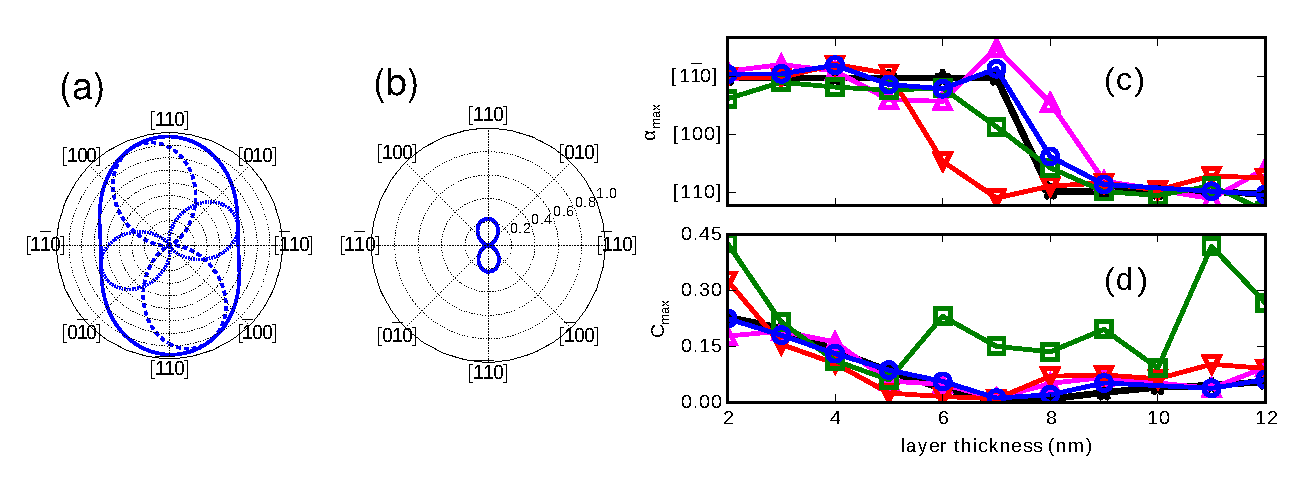
\includegraphics[width=1\linewidth]{/Sci_rep/test/a}
%	\caption{test}
%	\label{fig:kt_sectext}
%\end{figure}

%\newpage 





\section{Theory}

The Taylor expansion of ${\bf P}$ in terms of $\eta$ is obtained as
%
\begin{equation}
\label{eq:2ndPiezGeneral}
P_{\mu}=\sum_je_{\mu j}\eta_j+\frac{1}{2}\sum_{jk}B_{\mu jk}\eta_j\eta_k+\dots,
\end{equation}
%
where $e_{\mu j}$ is the linear and $B_{\mu jk}$ are the quadratic piezoelectric coefficients. In $\mathrm{III-V}$ zincblende semiconductors most of $e$ and $B$ coefficients are equal to each other and only one linear ($e_{14}$) and three non-linear ($B_{114}$, $B_{124}$, $B_{156}$) terms remain independent in Eq.~(\ref{eq:2ndPiezGeneral})~\cite{Beya-Wakata2011}. It is then convenient to rewrite Eq.~(\ref{eq:2ndPiezGeneral}) as ${\bf P}={\bf P}_{l}+{\bf P}_{nl}$, where ${\bf P}_{l}$ is the linear term:
%
%
\begin{equation}
\label{eq:1stPiez}
{\bf P}_{l}=e_{14}\begin{pmatrix}\eta_4\\\eta_5\\\eta_6\end{pmatrix},
\end{equation}
%
and ${\bf P}_{nl}$ the nonlinear one:
%
\begin{equation}
\label{eq:2ndPiez}
{\bf P}_{nl}=B_{114}\begin{pmatrix}\eta_1\eta_4\\\eta_2\eta_5\\\eta_3\eta_6\end{pmatrix}+
B_{124}\begin{pmatrix}\eta_4(\eta_2+\eta_3)\\\eta_5(\eta_3+\eta_1)\\\eta_6(\eta_1+\eta_2)\end{pmatrix}+
B_{156}\begin{pmatrix}\eta_5\eta_6\\\eta_4\eta_6\\\eta_4\eta_5\end{pmatrix}.
\end{equation}
%
%
Here $\eta$-s are indexed according to the Voigt notation,~i.~e.,~ $\eta_1=\eta_{xx}$, $\eta_2=\eta_{yy}$, $\eta_3=\eta_{zz}$, $\eta_4=2\eta_{yz}$, $\eta_5=2\eta_{xz}$, $\eta_6=2\eta_{xy}$~\cite{Beya-Wakata2011} where $x,y,z$ denote the crystallographic axes of the conventional cubic unit cell of the zincblende lattice.
%
%$1=xx,2=yy,3=zz,4=yz,5=xz,6=xy$~\cite{Beya-Wakata2011}.
%
Note that even though the coefficients of the expansion into cubic
%higher order 
terms were provided by Tse and colleagues~\cite{Tse2013}, we restrict ourselves to second-order ones here because of the small magnitude of the externally applied stress of only 0.1$\,$\%~\cite{Aberl:17} and, thus, we can describe experimental results obtained by Aberl~et~al.~\cite{Aberl:17} accurately within this restriction. 


\section{Single-particle calculations based on 8-band $\bf{k \cdot p}$ method}




%Before we present the results of full electronic structure calculations for the InGaAs QDs obtained by the nextnano$^3$ simulation suite~\cite{Birner:07}, we analyze the additional piezoelectric polarization established by the externally applied stress. In particular, we show that despite the small strains in the InGaAs layer occurring as a consequence of deformation of the piezo actuator bonded to the sample, the established piezo-polarization is dominated by the second order constants $B_{\mu,j,k}$. For simplicity, in this section we treat the InGaAs QD as two-dimensional layer with tetragonal symmetry.  
%


%For comparison to our simplified model, 
%
We have used the envelope function approximation based on 8-band ${\bf k}\cdot{\bf p}$ perturbation method using the nextnano$^3$ simulation suite~\cite{Birner:07}. The simulations can be divided into 4~following~steps:
%
\begin{itemize}
	\item [1.] definition of the simulation structure (shape, material parameters),
	\item[2.] calculations of the strain in the structure by minimization of the elastic energy,
	\item[3.] calculations of the electric field in the structure by solving the Poisson equation and calculation of the piezoelectric field,
	\item[4.] solving the single-electron Schrödinger equation using the envelope function approximation.
\end{itemize}
%
%We have calculated the electronic structure of InGaAs/GaAs QDs with the shape of truncated cones as shown in Fig.~\ref{fig:2order:QDStruct} using the envelope function approximation based on 8-band ${\bf k}\cdot{\bf p}$ perturbation method using the nextnano$^3$ simulation suite~\cite{Birner:07}. 
The calculations include full treatment of the elastic strain field employing the Bir-Pikus hamiltonian~\cite{BirPik}. Piezoelectric fields up to the second order in the strain are included self-consistently. Material parameters used in our simulations are listed in Appendix~\ref{app:material_params}. 





We have simulated two structures of InGaAs/GaAs QDs with the shapes of truncated cones that we call QD$_1$ and QD$_2$ differing in size and In alloy distribution.
%
\begin{figure}[!ht]
	\renewcommand{\tabcolsep}{2pt}
	\begin{center}
		\begin{tabular}{c}
			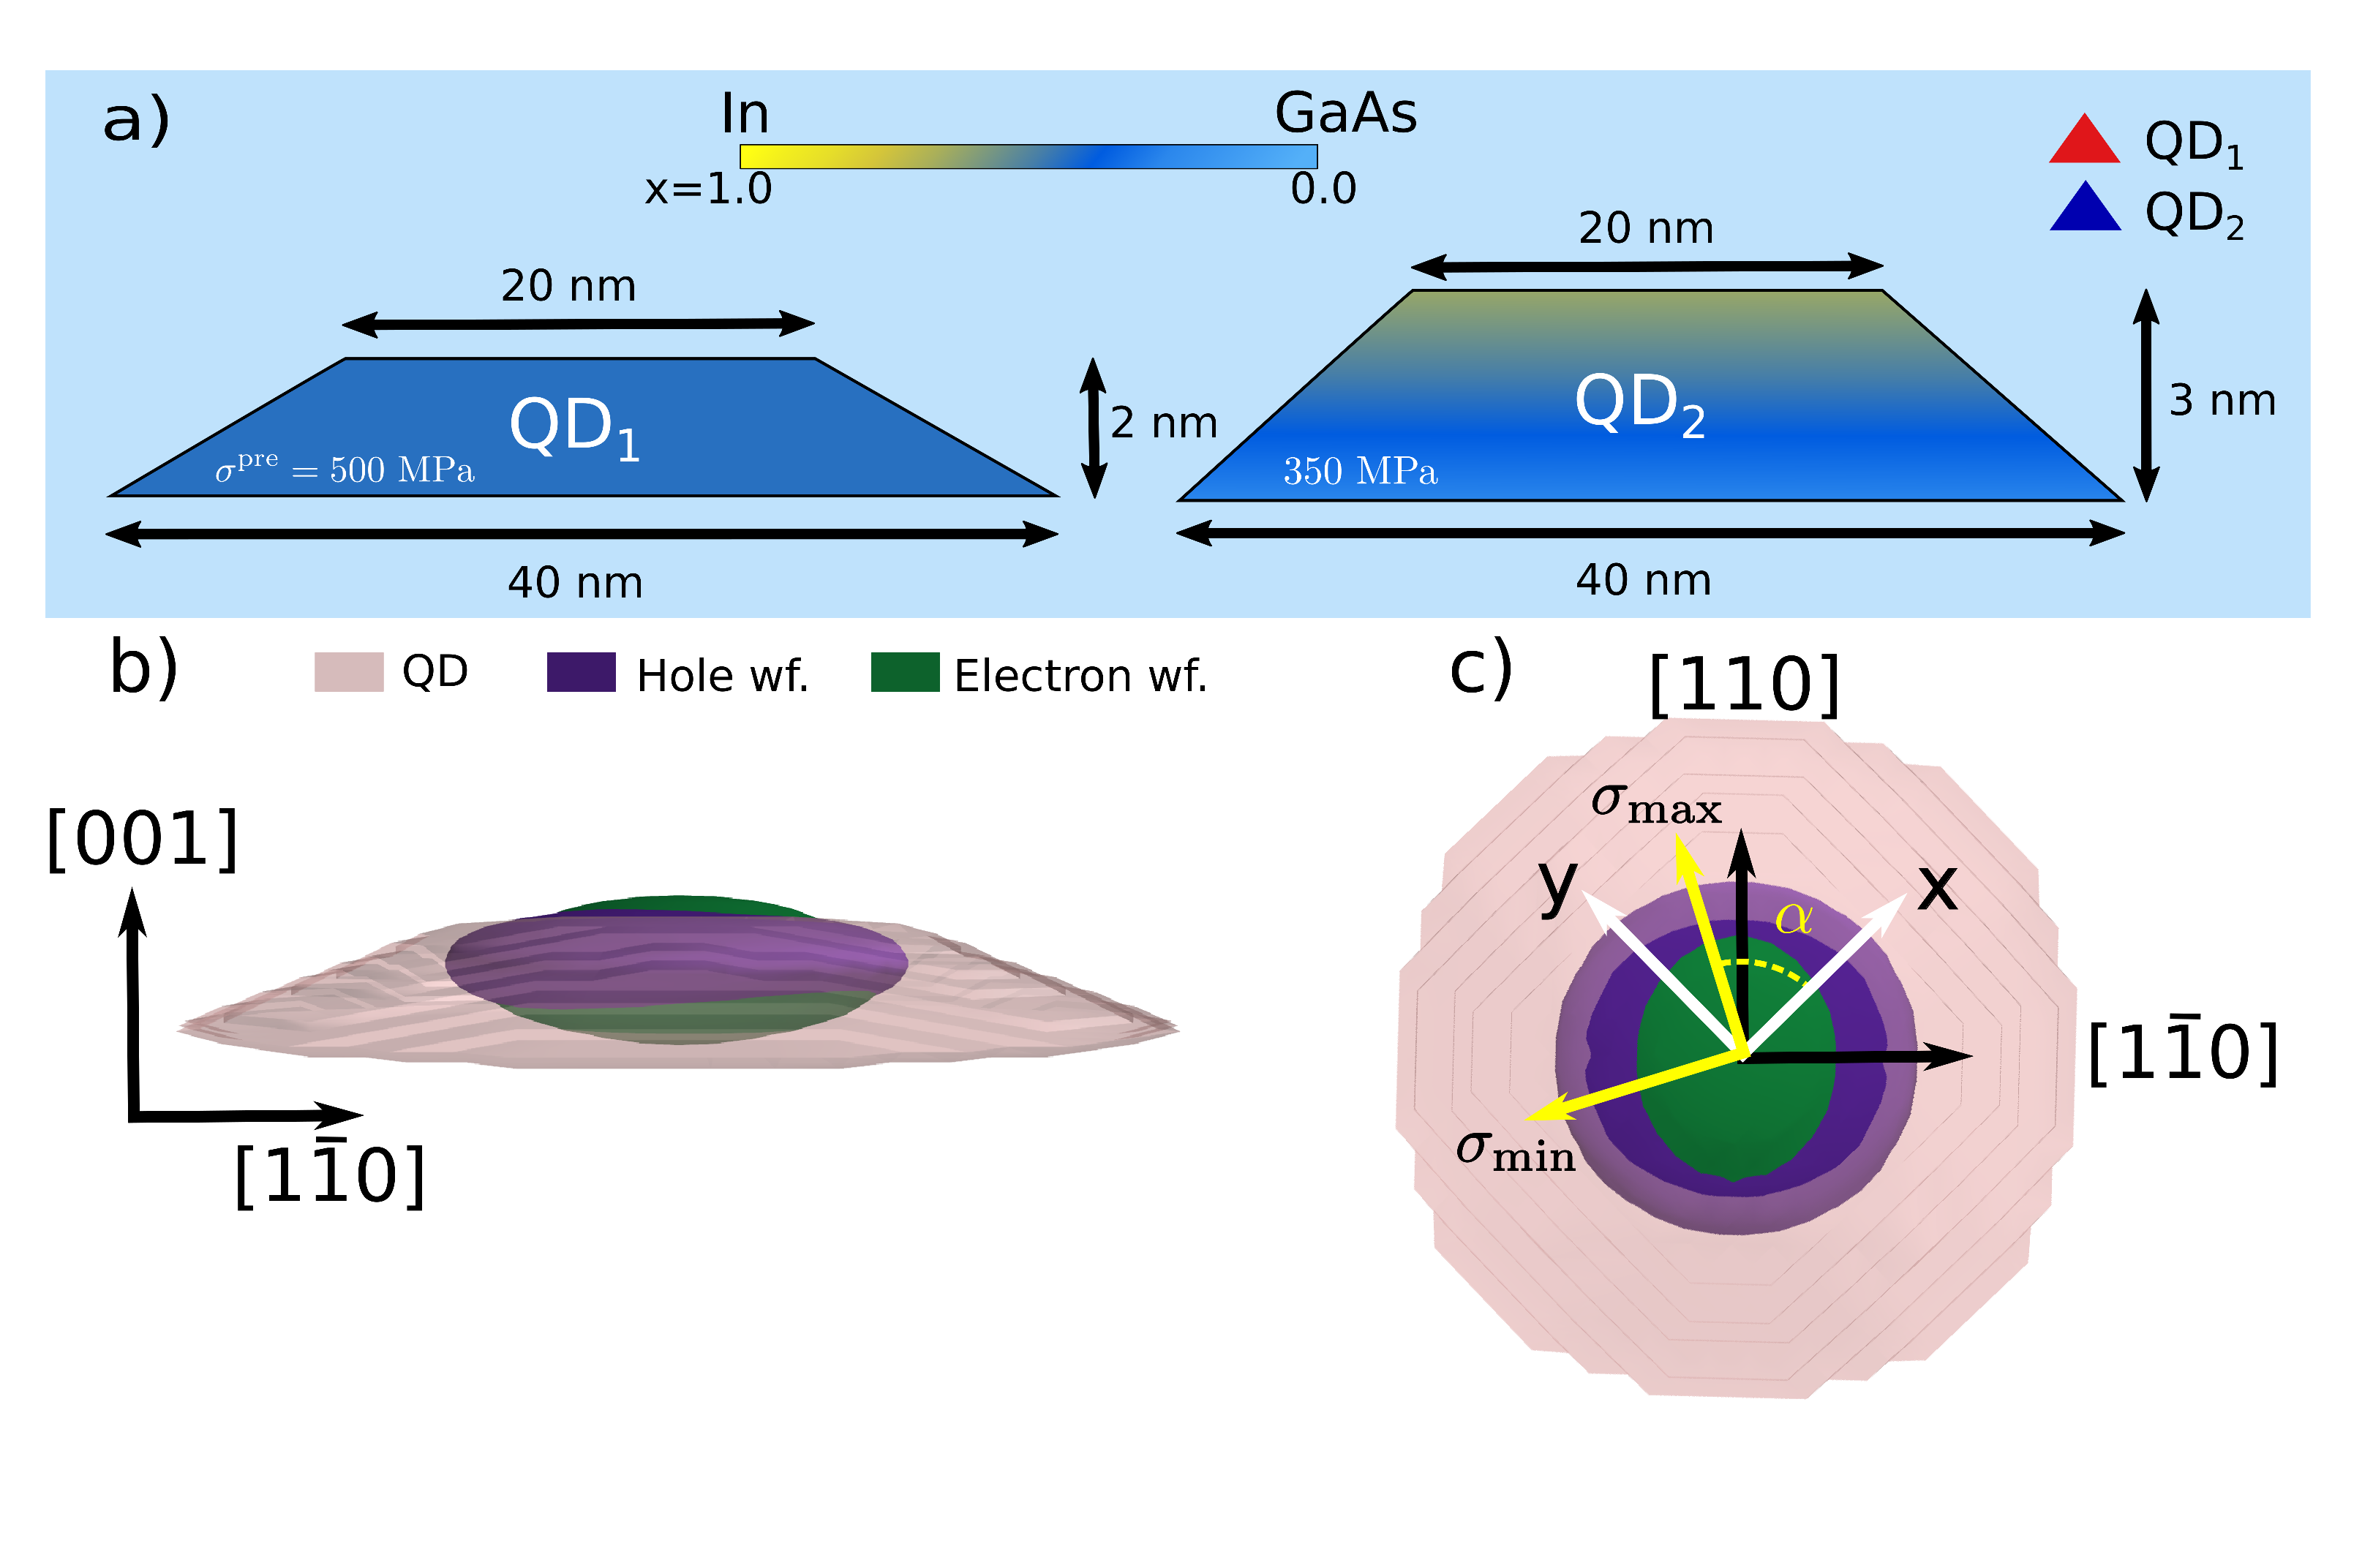
\includegraphics[width=0.8\textwidth]{2_order/180204_structura_wo-gradient_w_triangles_and_wfuncions_vs5} \\ 
		\end{tabular}
	\end{center}
	\caption{In panel a) we show the side view of the calculated In$_{{x}}$Ga$_{1-x}$As/GaAs QD$_1$ and QD$_2$ structures. Both QDs have the shape of truncated cones with base and top diameters of 40$\,$nm and 20$\,$nm, respectively, the height is 2$\,$nm~(3$\,$nm), In composition is constant of 0.45 (linearly increasing from 0.25 at the bottom to 0.65 at the apex), and $\sigma^\text{pre}=500$$\,$MPa ($\sigma^\text{pre}=350$$\,$MPa) for QD$_1$ (QD$_2$). Panels b) and c) show the side and top view, respectively, of the typical simulated dot (pink), and calculated electron (green) and hole (blue) probability densities. The wavefunctions are given as isosurfaces encircling 70\% of the total probability.
		\label{fig:2order:QDStruct}}
\end{figure}

Side views of QD$_1$ and QD$_2$ are shown in Fig.~\ref{fig:2order:QDStruct}~a) and their parameters were deliberately chosen so that the calculated dependencies of the emission energy $E_0$ and of the dipole moment $p$ on the hydrostatic part of the applied anisotropic stress $\sigma_{\mathrm{max}}+\sigma_{\mathrm{min}}$ match the experimental results taken from Ref.~\cite{Aberl:17}, see Fig.~\ref{fig:TheorVsExp}. The variables $\sigma_{\mathrm{max}}$ and $\sigma_{\mathrm{min}}$ denote the principal stresses~\cite{Trotta:15} applied externally by the two-dimensional piezo actuator. In  Ref.~\citep{Aberl:17} it was shown that $\sigma_{\mathrm{max}}$ was applied at an angle of $\alpha=55\,^{\circ}$ with respect to the crystal axis [100], resulting in the principal axis system of the externally applied stress as shown in Fig. \ref{fig:2order:QDStruct}. The various coordinate systems used in our model as well as the single-particle wavefunctions of electrons and holes are indicated in Fig. \ref{fig:2order:QDStruct} b) and c). The connection between the Cartesian and the principal stresses is derived in~Appendix~\ref{app:principal_stress}.

As discussed in Ref.~\cite{Aberl:17}, in course of bonding the sample onto the piezo actuator, a~shear prestess $\sigma^\text{pre}$ independent on the voltage applied to the piezo is exerted on the sample. Consequently, in order to match the measured values of $p$ with results of our calculations we needed to allow for different magnitude of $\sigma^\text{pre}$ of 500 and 350$\,$MPa that acted on QD$_1$ and QD$_2$, respectively.

Experimentally acquired dependencies of $p/e$ on $\sigma_{\mathrm{max}}+\sigma_{\mathrm{min}}$ shown in Fig.~\ref{fig:TheorVsExp} follow a linear behavior, therefore, we have fitted the (gray) data by linear model derived by {Kle\-no\-vský~et~al.}~\cite{Klenovsky_2018_InGaAs_straintuned}
%
\begin{eqnarray}
p/e\approx A^{\mathrm{QD}}\left(\sigma_\mathrm{max}+\sigma_\mathrm{min}\right)+b, \label{eq:strain_model}
\end{eqnarray}
%
which allows us to describe the evolution of $p/e$ by two constants $A^{\mathrm{QD}}$ and $b$. Results of the fit by model~(\ref{eq:strain_model}) are listed in Tab.~\ref{tab:exp_slopes} in Appendix~\ref{app:slopes_of_dipole}.

%


\begin{figure}[!ht]
	\centering
	\renewcommand{\tabcolsep}{2pt}
	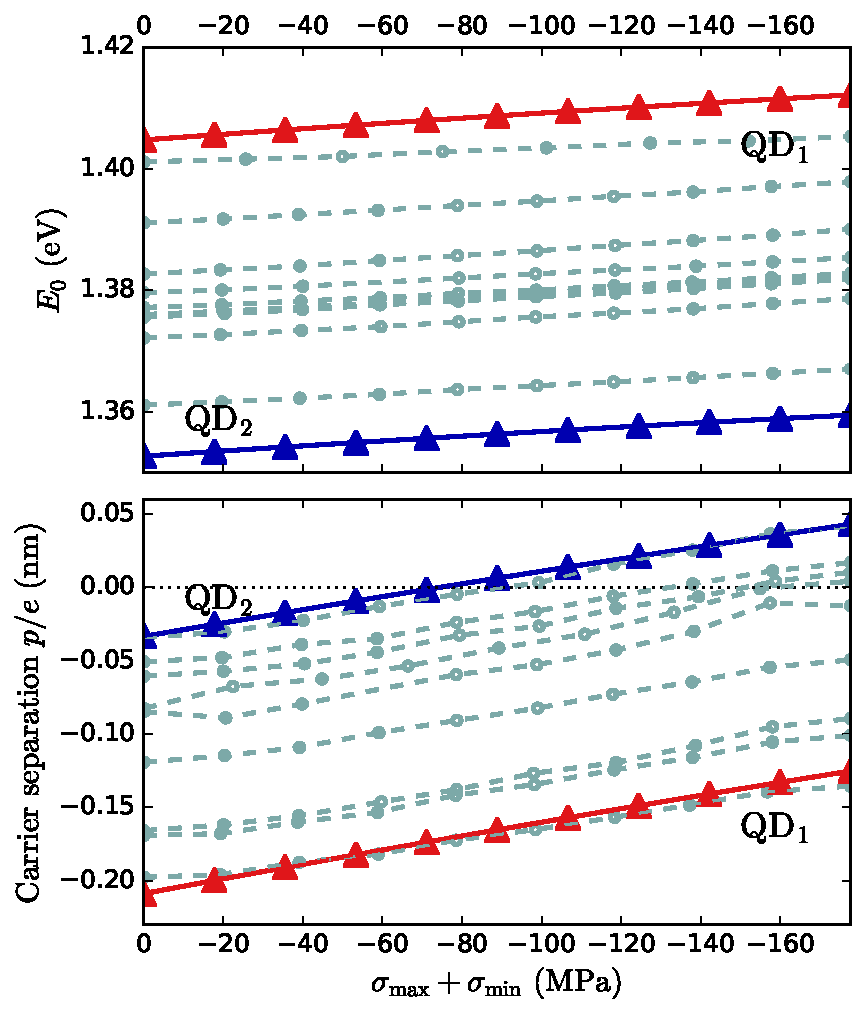
\includegraphics[width=0.5\textwidth]{/2_order/Energy/2018-04-25__171219_8x8_neotocena_++_nn+_35deg_pres500___theoryVSexperiment} 
	\caption{
		Dependencies of $E_0$ (top panel) and $p/e$ (bottom panel) on $\sigma_{\mathrm{max}}+\sigma_{\mathrm{min}}$ experimentally obtained from $\mu$PL measurements of nine InGaAs QDs~\cite{Aberl:17} (dashed curves) and that calculated for QD$_1$ (full red curve) and QD$_2$ (full blue curve). The letter $e$ denotes the elementary charge.}
	%
	%two different QDs, i.e. first with base and top diameter of 30~nm and 15~nm, respectively and height of 3~nm. 
	\label{fig:TheorVsExp}
\end{figure}

\newpage

\section{Effect of second order of piezoelectricity}
%
\begin{figure}[h]
	%\renewcommand{\tabcolsep}{2pt}
	\begin{center}
		\begin{tabular}{cc}
			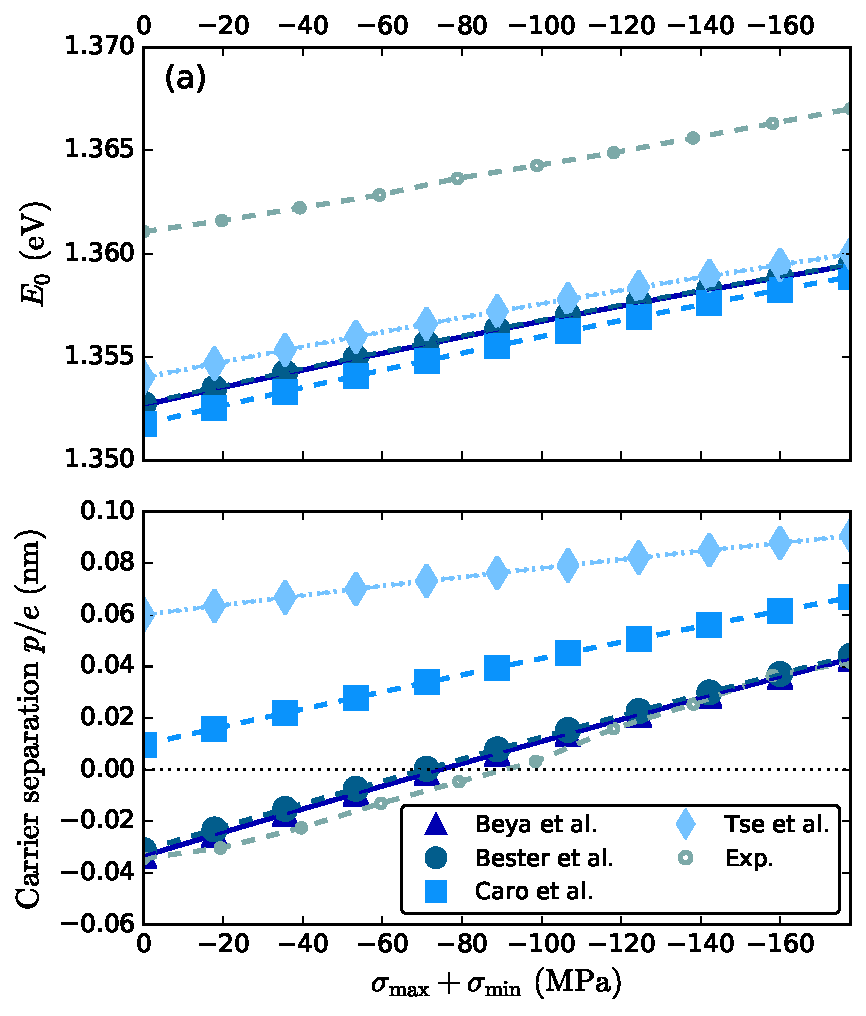
\includegraphics[width=0.5\textwidth]{/2_order/Energy/FINAL_a__171219_8x8_neotocena_++_nn+_35deg_pres350___40x20x3-25-65_350_piezo2ndorder} & 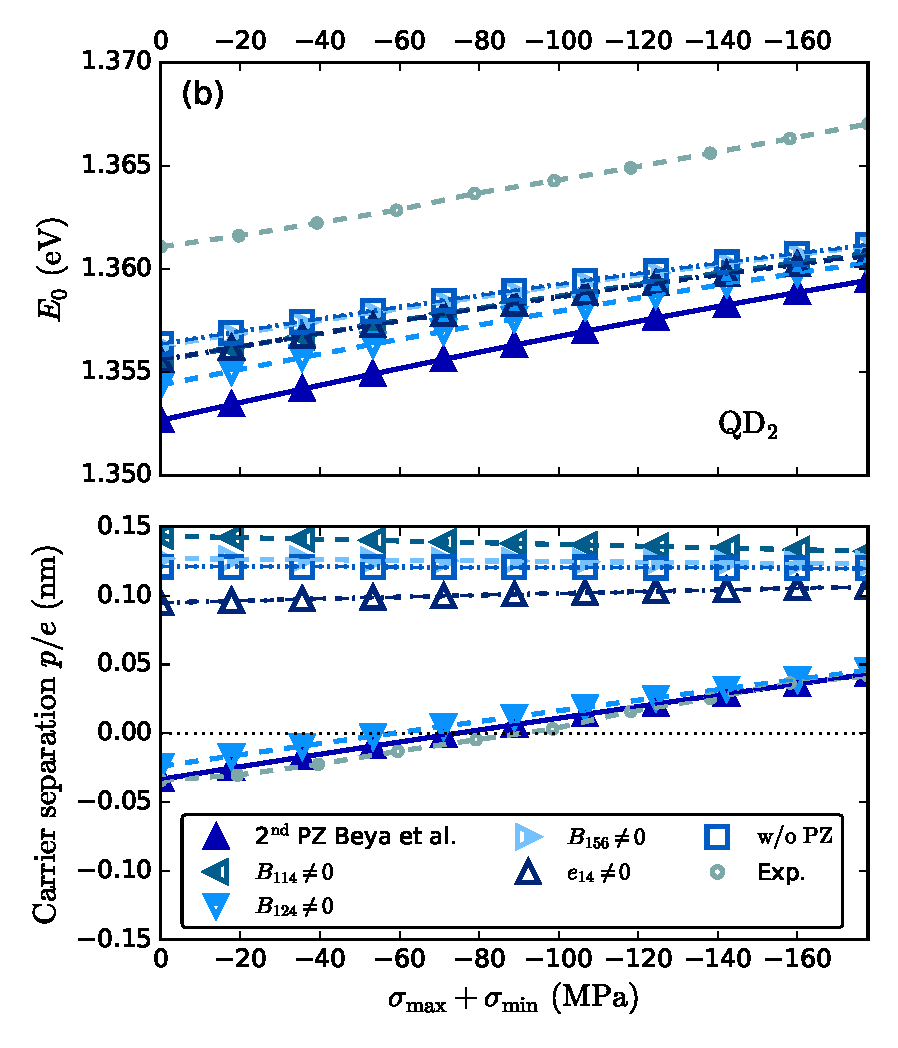
\includegraphics[width=0.5\textwidth]{/2_order/Energy/FINAL_b__171219_8x8_neotocena_++_nn+_35deg_pres350___40x20x3d0_piezo2ndorder_jednotlive_cleny}\\
		\end{tabular}
	\end{center}
	\caption{
		(a) Comparison of calculated results based on four published sets of parameters of second order piezoelectric coefficients, i.~e., Refs.~\cite{Beya-Wakata2011,Bester:06,Caro2015,Tse2013} for QD$_2$. (b) Comparison of dependencies of $E_0$ and $p/e$ on $\sigma_{\mathrm{max}}+\sigma_{\mathrm{min}}$ for all piezoelectric parameters equal to zero except for $e_{14}$, $B_{114}$, $B_{124}$, and $B_{156}$ sequentially retaining their values for QD$_2$. In both (a) and (b) we show the dependencies of $E_0$ on applied stress $\sigma_{\mathrm{max}}+\sigma_{\mathrm{min}}$ in the upper panels and that for $p/e$ in lower ones. 
		The experimental data from Ref.~\cite{Aberl:17} are shown by the grey dashed curves in all panels. 
		\label{fig:DiffPiezo}}
\end{figure}


In Ref.~\cite{Aberl:17} it was discussed that the experimentally obtained values of the dependence of $p/e$ on $\sigma_{\mathrm{max}}+\sigma_{\mathrm{min}}$ can be explained only by including the second-order contribution to the piezoelectric field.
%
Motivated by that, we proceed with the analysis of the evolution of $p/e$ on $\sigma_{\mathrm{max}}+\sigma_{\mathrm{min}}$ for all published second-order piezoelectric parameters listed in Tab.~\ref{tab:second_piez_param}. 
%
%
\begin{table*}[!ht]
	\begin{center}
		\caption{Values for the linear and quadratic piezoelectric coefficients $e_{14}$, $B_{114}$, $B_{124}$ and $B_{156}$. The references from which the parameters were taken are identified in the first column. The units of presented piezoelectric constants are $C/m^2$. For In$_x$Ga$_{1-x}$As, the constants were obtained by linear interpolation.
		\label{tab:second_piez_param}	
		}
		\begin{tabular}{c|ccccc}
			\hline \hline
			%Ref. & compound & $e_{14}$ $(C/m^2)$& $B_{114}$ $(C/m^2)$ & $B_{124}$ $(C/m^2)$&$B_{156}$ $(C/m^2)$\\
			Ref. & compound & $e_{14}$ & $B_{114}$  & $B_{124}$ &$B_{156}$\\
			\hline
			\multirow{2}{*}{Beya-Wakata et al.~\cite{Beya-Wakata2011}} & GaAs & $-0.238$ & $-0.4$  & $-3.8$& $-0.7$\\
			& InAs& $-0.115$ & $-0.6$  & $-4.1$& $0.2$\\
			% 
			\hline
			\multirow{2}{*}{Bester et al.~\cite{Bester:06} }& GaAs & $-0.23$ & $-0.439$  & $-3.765$& $-0.492$\\
			& InAs& $-0.115$ & $-0.531$  & $-4.076$& $-0.12$\\
			%
			\hline
			\multirow{2}{*}{Caro et al.~\cite{Caro2015}} & GaAs & $-0.205$ & $-0.99$  & $-3.21$& $-1.28$\\
			& InAs& $-0.111$ & $-1.17$  & $-4.31$& $-0.46$\\
			%		
			\hline
			\multirow{2}{*}{Tse et al.~\cite{Tse2013}} & GaAs & $-0.16$ & $-0.666$  & $-1.646$& $-$\\
			& InAs& $-0.045$ & $-0.653$  & $-1.617$& $-$\\
			\hline \hline
		\end{tabular}
	\end{center}
\end{table*}
%
%
The results for QD$_2$ are shown in Fig.~\ref{fig:DiffPiezo}~(a) and demonstrate that both the evolution of $p/e$ with $\sigma_{\mathrm{max}}+\sigma_{\mathrm{min}}$ as well as the slopes $\frac{1}{e}\partial p/\partial(\sigma_{\mathrm{max}}+\sigma_{\mathrm{min}})$ and $\partial E_0/\partial(\sigma_{\mathrm{max}}+\sigma_{\mathrm{min}})$ remain remarkably similar among various parameter sets in the literature even though the coefficients differ considerably among them.
For example, the parameter $B_{156}$ has even a different sign between Refs.~\cite{Bester:06} and~\cite{Beya-Wakata2011} or is omitted in Ref.~\cite{Tse2013}.
%


%
%\begin{figure}
%	\begin{center}
	%	\includegraphics[width=0.42\textwidth]{/2_order/FINAL__171219_8x8_neotocena_++_nn+_35deg_pres350___40x20x3d0_piezo2ndorder_jednotlive_cleny}
	%\end{center}
	%\caption{
	%	Comparison of dependencies of $E_0$ and $p/e$ on $\sigma_{\mathrm{max}}+\sigma_{\mathrm{min}}$ for all piezoelectric parameters equal to zero except for $e_{14}$, $B_{114}$, $B_{124}$, and $B_{156}$ sequentially retaining their values for QD$_2$. For comparison, one set of the experimental data from Ref.~\cite{Aberl:17} is given by the grey dashed curve. Otherwise the outline of the figure is the same as that in Fig.~\ref{fig:DiffPiezo}.
	%	\label{fig:DiffPiezoCoeff}}
%\end{figure}


To investigate the origin of that apparent similarity we have performed calculations, in which we have set all piezoelectric parameters equal to zero except for $e_{14}$, $B_{114}$, $B_{124}$, and $B_{156}$ sequentially retaining their values, see Fig.~\ref{fig:DiffPiezo}~(b) for those results for QD$_2$. 


Firstly, we note that the dependencies for $E_0$ are very similar irrespective of which piezoelectric parameter is not set to zero. This is connected with the fact that a change of the emission energy from QDs with stress is dominated by the hydrostatic components.

Secondly, the most important piezoelectric parameter is noticeably $B_{124}$. Evidently, the second term in Eq.~(\ref{eq:2ndPiez}) dominates the dependencies of $E_0$ and $p/e$ on $\sigma_{\mathrm{max}}+\sigma_{\mathrm{min}}$. This is not surprising since the magnitude of $B_{124}$ is several times larger than that of $e_{14}$, $B_{114}$, or $B_{156}$~\cite{Beya-Wakata2011}, see Tab.~\ref{tab:second_piez_param}. 


\section{Effect of indium distribution}

\begin{figure}[!ht]
	\renewcommand{\tabcolsep}{2pt}
	\begin{center}
		\begin{tabular}{c}
			%\includegraphics[width=0.4\textwidth]{2017-12-15__170921_35deg_pres200___30x15x3_concentration.eps} \\
			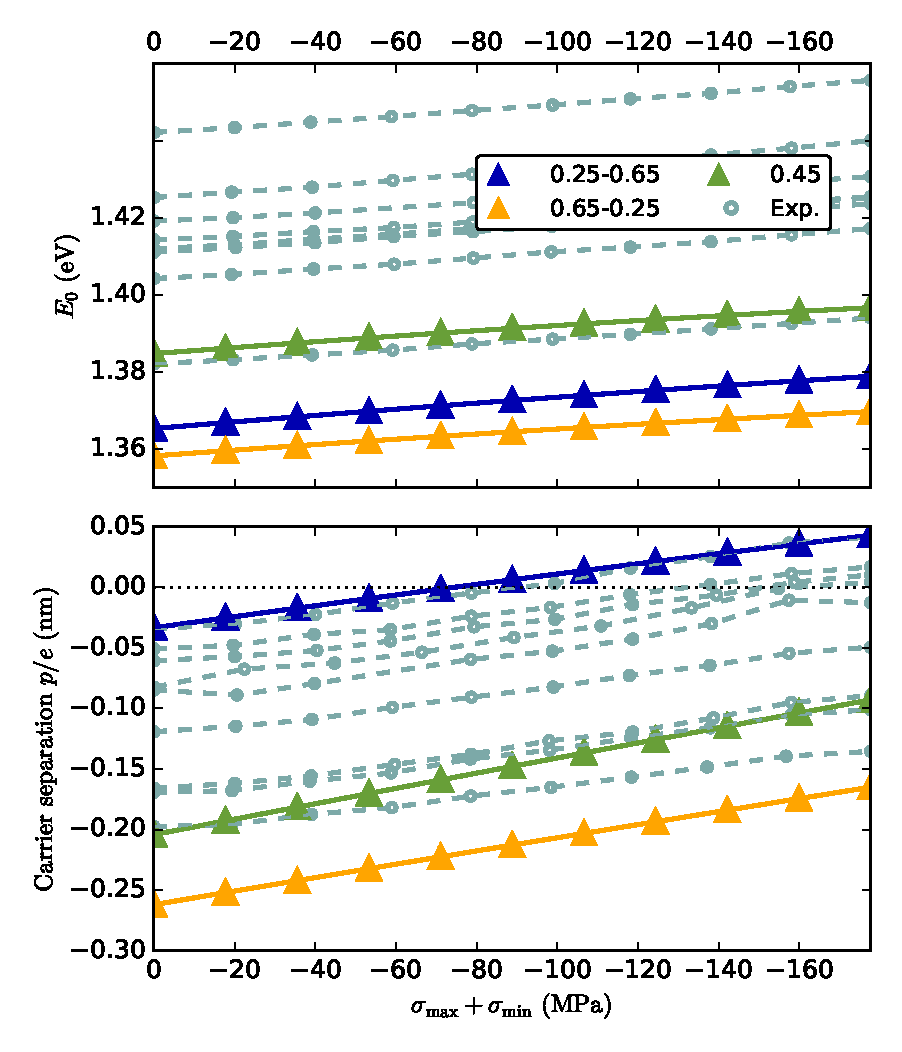
\includegraphics[width=0.5\textwidth]{/2_order/Energy/FINAL__171219_8x8_neotocena_++_nn+_35deg_pres350___40x20x3_concentration} \\
		\end{tabular}
	\end{center}
	\caption{
		Dependencies of $E_0$ (top panel) and $p/e$ (bottom panel) on $\sigma_{\mathrm{max}}+\sigma_{\mathrm{min}}$ experimentally obtained from $\mu$PL measurements of nine InGaAs QDs~\cite{Aberl:17} (dashed curves) and that calculated for different In contents inside QD. The data for In content linearly varying as a function of vertical dimension from 0.25~(0.65) at QD base to 0.65~(0.25) at QD apex are shown as blue~(orange) curves. Those for constant In content of 0.45 are given as green curves. The data calculated assuming second-(first-)order piezoelectricity taken from Ref.~\citep{Beya-Wakata2011} are given as full (open) symbols. All other properties of the dots were the same as for QD$_2$. The letter $e$ denotes the elementary charge.
		\label{fig:TuningByConc}}
\end{figure}
%

Motivated by Refs.~\cite{Grundmann, Fry:00} discussing the influence of indium distribution inside {InGaAs/GaAs} QDs on $p$ we have also studied the effect of that in our stress-tuned dots. In Fig.~\ref{fig:TuningByConc} we show $E_0$ and $p$ as a function of $\sigma_{\mathrm{max}}+\sigma_{\mathrm{min}}$ for In contents (i) linearly increasing from 0.25 at the QD base to 0.65 at its apex, (ii) the same but for reverted concentration profile and (iii) for constant In composition of 0.45. Clearly, we find that $p/e$ where $e$ is the elementary charge at $\sigma_{\mathrm{max}}+\sigma_{\mathrm{min}}=0$ can be varied considerably by changing the slope of In content from $-0.03$$\,$nm for (i) to $-0.26$$\,$nm for (ii). The case (iii) is found in between at $-0.20$$\,$nm. Note that previous values were obtained assuming the second-order piezoelectricity. The data calculated with only first-order piezoelectricity show similar trends in agreement with the results of Refs.~\cite{Grundmann, Fry:00}. Noticeably, both $E_0$ and $\partial E_0/\partial(\sigma_{\mathrm{max}}+\sigma_{\mathrm{min}})$ do not depend appreciably on In distribution and only the mean value of In concentration is important.

However, the slopes $\frac{1}{e}\partial p/\partial(\sigma_{\mathrm{max}}+\sigma_{\mathrm{min}})$ differ considerably in case of first- and second-order piezoelectricity. We find the values of the fitted slopes in the former case in the range from 0.074 to 0.1$\,$nm/GPa while for the latter they are between 0.42 and 0.55$\,$nm/GPa. Slopes of the experimental data are between 0.42 and 0.5$\,$nm/GPa. The relative error of all fitted slopes is $\approx 5$$\,$\%, see also Tab.~\ref{tab:conc_slopes} in Appendix~\ref{app:slopes_of_dipole} for the list of all fitted values and their errors. Thus, very good agreement is found between calculations assuming second-order piezoelectricity and experiment rather than for the first-order. % We will return to this point in the following.


\section{Effect of bonding prestress}
\begin{figure}[!ht]
	\renewcommand{\tabcolsep}{2pt}
	\begin{center}
		\begin{tabular}{c}
			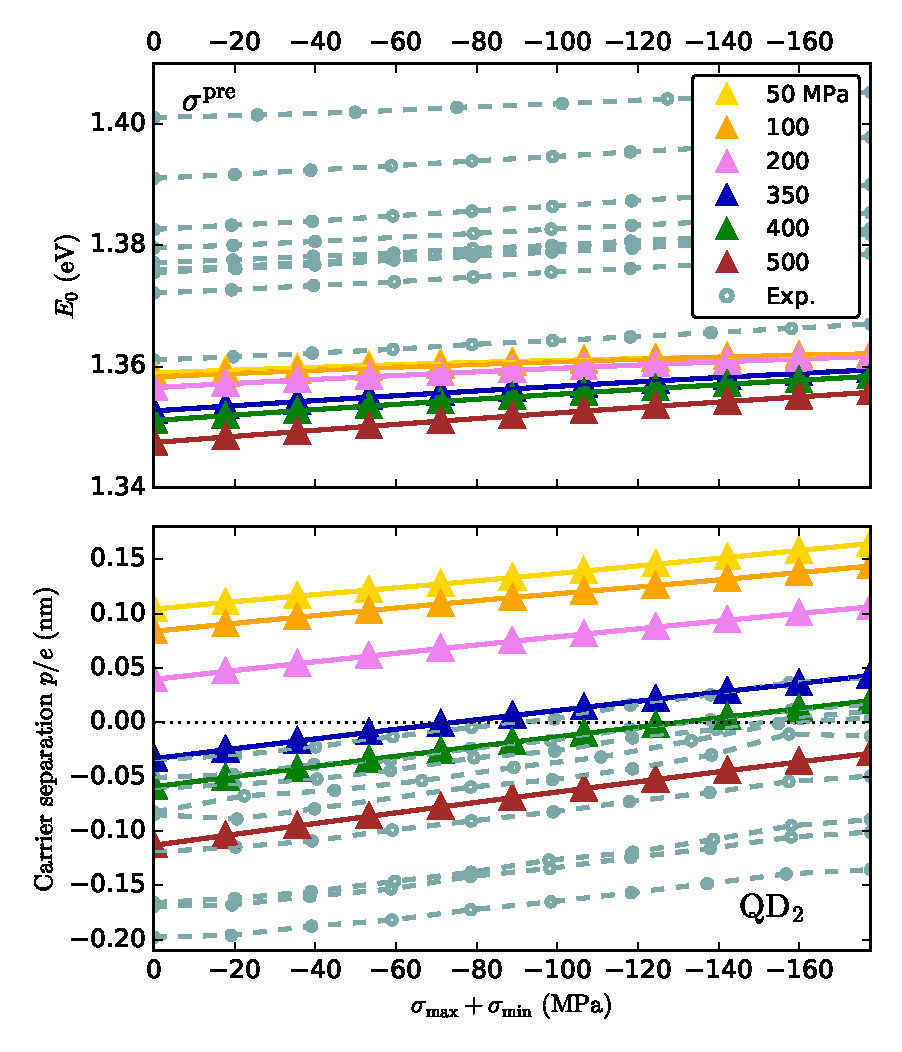
\includegraphics[width=0.5\textwidth]{/2_order/Energy/FINAL__171219_8x8_neotocena_++_nn+_35deg_pres500___prestress} \\
		\end{tabular}
	\end{center}
	\caption{
		Dependencies of $E_0$ (top panel) and $p/e$ (bottom panel) on $\sigma_{\mathrm{max}}+\sigma_{\mathrm{min}}$ experimentally obtained from $\mu$PL measurements of nine InGaAs QDs~\cite{Aberl:17} (dashed curves) and that calculated for different values of $\sigma^{\mathrm{pre}}$. Except for $\sigma^{\mathrm{pre}}$ the simulated QDs had the same properties as QD$_2$. The letter $e$ denotes the elementary charge.
		\label{fig:TuningByPrestress}}
\end{figure}
%
Noticeably, the work in Ref.~\cite{Klenovsky_2018_InGaAs_straintuned} pointed to the importance of prestress $\sigma^\mathrm{pre}$ caused by bonding of the sample onto the piezo actuator. The bonding quality was shown to significantly affect FSS measured during stress-tuning.
%
%, which can be reproduces reas with increasing $\sigma^\mathrm{pre}$. 
%The minimal value 1.15~$\mu$eV of FSS was reached for $\sigma^{\mathrm{pre}}=50$~MPa.




In bottom panel of Fig.~\ref{fig:TuningByPrestress} we show $p/e$ for different values of $\sigma^{\mathrm{pre}}$ acting on QD$_2$. The values of $b$ taken from the fit of dependence of $p/e$ on ${\sigma_{\mathrm{max}}+\sigma_{\mathrm{min}}}$ by linear model~(\ref{eq:strain_model}) decrease with increasing $\sigma^\text{pre}$. Interestingly, $p/e$ attains positive values for  $\sigma^\text{pre}\lesssim 200$$\,$MPa. However, larger values of $\sigma^\text{pre}$ lead to negative values of $p/e$ for $\sigma_{\mathrm{max}}+\sigma_{\mathrm{min}}=0$. 

While $\sigma^{\mathrm{pre}}$ considerably influences the overall magnitude of $p$ it only mildly affects the slope $A^{\mathrm{QD}}$ or the values of $E_0$.
%
%
%

\begin{figure}[!ht]
	\renewcommand{\tabcolsep}{2pt}
	\begin{center}
		\begin{tabular}{c}
			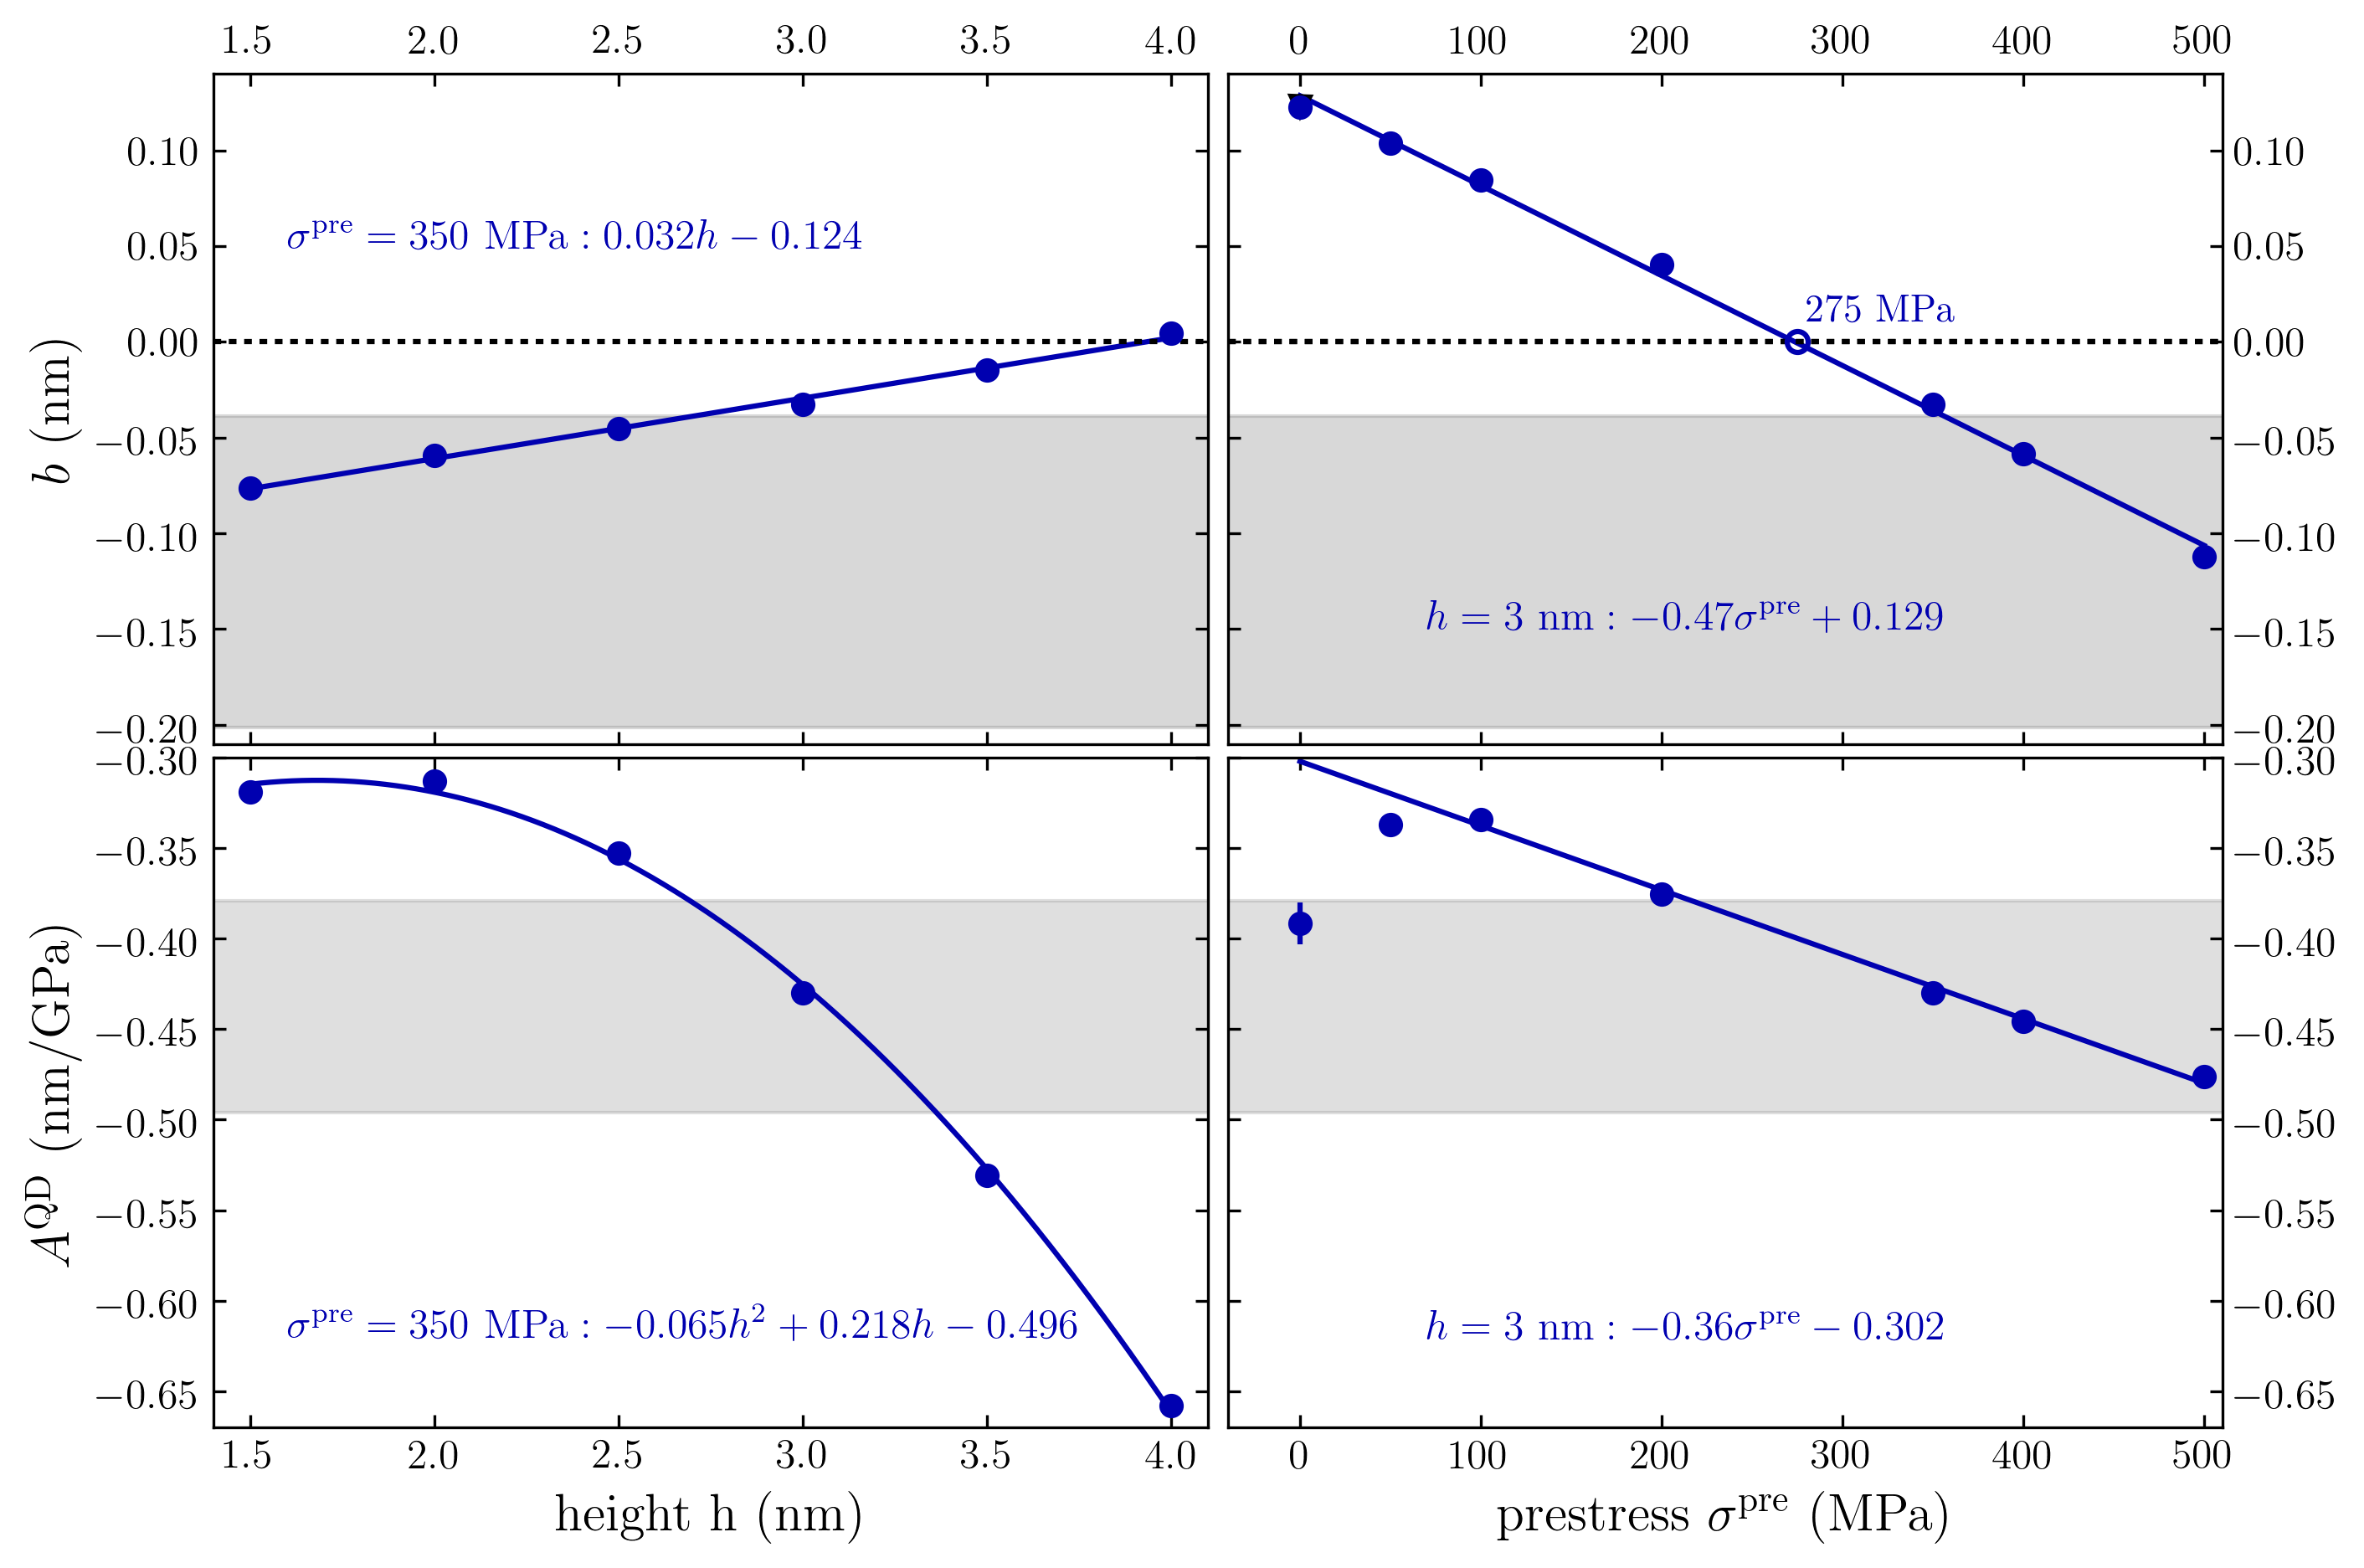
\includegraphics[width=0.9\textwidth]{/2_order/Height_Prestres_fit_pars_3} \\
		\end{tabular}
	\end{center}
	\caption{Evolution of parameters $A^{\mathrm{QD}}$ and $b$ obtained using linear fit $p/e$ on $\sigma_{\mathrm{max}}+\sigma_{\mathrm{min}}$ for varying height of QD (left column) and applied $\sigma^{\mathrm{pre}}$ (right column). Full marks represent values obtained from $\mathbf{k\cdot p}$ calculations, solid lines are fits of the values, and empty symbols point to the values $\sigma^\mathrm{pre}_\mathrm{0}$ where the inversion of $p$ occurs. The grey (yellow) shaded area indicates interval of values observed in $\mu$PL measurements (interval of saturated values of $A^{\mathrm{QD}}$). 
		\label{fig:FitHeightPrestress}}
\end{figure}
%
For a more detailed analysis of the parameters $A^{\mathrm{QD}}$ and $b$ we plot those as a function of $\sigma^{\mathrm{pre}}$ and dot height $h$ and fit them by the linearly decreasing function~(\ref{eq:strain_model}), see resulting parameters in Fig.~\ref{fig:FitHeightPrestress}. The fitted values of the linear model are added in Appendix~\ref{app:empirical_model} in Tab.~\ref{tab:prestress_fit}.

The parameter $b$ can be expressed as a sum of two contributions
\begin{eqnarray}
b =\frac{1}{e} \left(p^\mathrm{pre} + p^\mathrm{QD}\right)=b_1\sigma^\mathrm{pre} +b_0,
\end{eqnarray} 
%
%
where $p^\mathrm{QD}$ is QD dipole without bonding and applied stress, $p^\mathrm{pre}$ is the effect on $p$ of QD created by adding the sample onto the piezo actuator which we assume to be independent on the applied voltage on the piezo~\cite{Aberl:17}. Because $\sigma^{\mathrm{pre}}$ acts against the applied stress $\sigma_{\mathrm{max}}+\sigma_{\mathrm{min}}$ this results in a decrease of $b$ with increasing $\sigma^\mathrm{pre}$. On the other hand, increasing QD height enables the charge carriers to relax more in vertical direction in QD body causing an increase of $b_0=\frac{1}{e}\times p^\mathrm{QD}$. Interestingly, dependencies of $b$ on $\sigma^\mathrm{pre}$ for several QD heights intersect for $\sigma^\mathrm{pre}=500$$\,$MPa.

%
%
Moreover, using the above described approach we can estimate more precisely $\sigma^\mathrm{pre}_\mathrm{0}$ for which the inversion of $p$ occurs. For example, for QD$_2$ we have found $\sigma^\mathrm{pre}_\mathrm{0}=275$$\,$MPa. 
%Interestingly, 
Noticeably, for all dependencies of parameter $A^{\mathrm{QD}}$ on $\sigma^\mathrm{pre}_\mathrm{0}$ we observe an increase in $A^{\mathrm{QD}}$ saturating for some value $\sigma^\mathrm{pre}_\mathrm{c}$, followed again by a linear decrease of $A^{\mathrm{QD}}$, similarly as for the dependencies of $b$. This is a result of using a quadratic dependence of ${\bf P}$ and, thus, $p$ on applied anisotropic stress, see Eq.~(\ref{eq:2ndPiez}).
%
%Unfortunately, so far we have no satisfying physical model of that behavior.

%Similar linear decrease we observe also for $A^{\mathrm{QD}}$ for , .











%








\section{Effect of quantum dot size}

%The emission and dipole moment $p$ of QDs are very sensitive to change not only material composition but also geometrical parameters.
In this section we will focus on tuning of $p$ and $E_0$ by QD height, aspect ratio, or diameter.
%
Firstly, we show the calculations for a set of heights of QD$_2$ in Fig.~\ref{fig:TuningByHeight}. We note that emission energies $E_0$ are smaller for larger heights similarly as in Ref.~\cite{t_schliwa} and can reproduce experimentally obtained $E_0$ in the whole measured range of $\sigma_{\mathrm{max}}+\sigma_{\mathrm{min}}$. Note that the decrease of $E_0$ with increasing QD height is expected since an increase of the latter with other QD parameters set fixed leads effectively to \enquote{widening} of the effective quantum well for quasiparticles in vertical direction.
%
%
\begin{figure}[ht!]
	\renewcommand{\tabcolsep}{2pt}
	\begin{center}
		\begin{tabular}{c}
			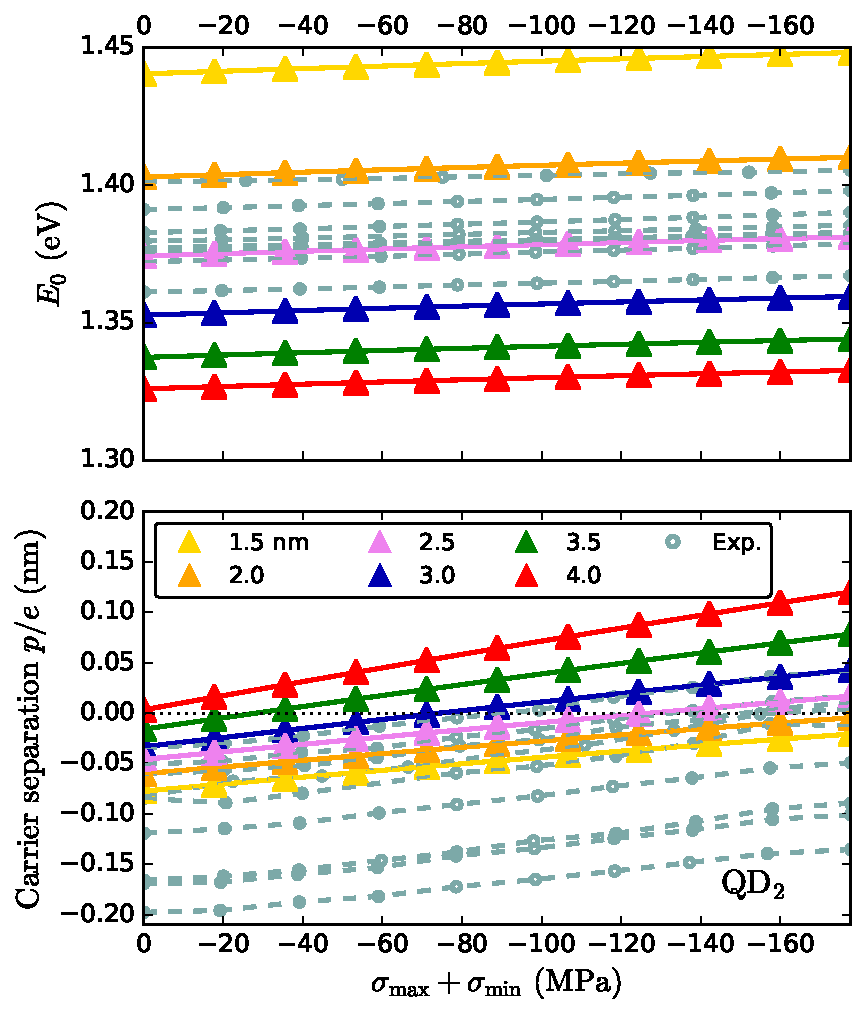
\includegraphics[width=0.5\textwidth]{/2_order/Energy/FINAL__171219_8x8_neotocena_++_nn+_35deg_pres350___40x20_height} \\
		\end{tabular}
	\end{center}
	\caption{
		Dependencies of $E_0$ (top panel) and $p/e$ (bottom panel) on $\sigma_{\mathrm{max}}+\sigma_{\mathrm{min}}$ experimentally obtained from $\mu$PL measurements of nine InGaAs QDs~\cite{Aberl:17} (dashed curves) and that calculated for different values of dot height. Except for height the simulated QDs had the same properties as QD$_2$ including the value of $\sigma^{\mathrm{pre}}=350$$\,$MPa. The letter $e$ denotes the elementary charge.
		\label{fig:TuningByHeight}}
\end{figure}

However, the dot height influences both $A^{\mathrm{QD}}$ and $b$ parameters in the dependency of $p/e$ on $\sigma_{\mathrm{max}}+\sigma_{\mathrm{min}}$. While $b$ is modified only slightly from $-0.076$ to $0.005$$\,$nm when changing $\sigma_{\mathrm{max}}+\sigma_{\mathrm{min}}$ from $-177$ to $0$$\,$MPa, at the same time $A^{\mathrm{QD}}$ increases dramatically from $-0.66$ to $-0.32$.




%
%

%

Finally, in Fig.~\ref{fig:TuningByLateral} we show the effect of variations in the lateral dimensions of QDs. In panel~(a) we change both the diameter of upper and lower plane for a fixed ratio of those, and in panel~(b) we vary the ratio of dimensions of upper and lower plane for fixed diameter of the latter.


%changes of the base top diameters of the QD truncated cone lead to absolute shifts of $E_0$ and $p/e$ but neither lateral dimension nor aspect (ratio between top and base radius) of QD entail variation in slopes of both quantity which is demonstrated in Fig.~\ref{fig:TuningByLateral}.

\begin{figure}[!ht]
	\renewcommand{\tabcolsep}{2pt}
	\begin{center}
		\begin{tabular}{cc}
			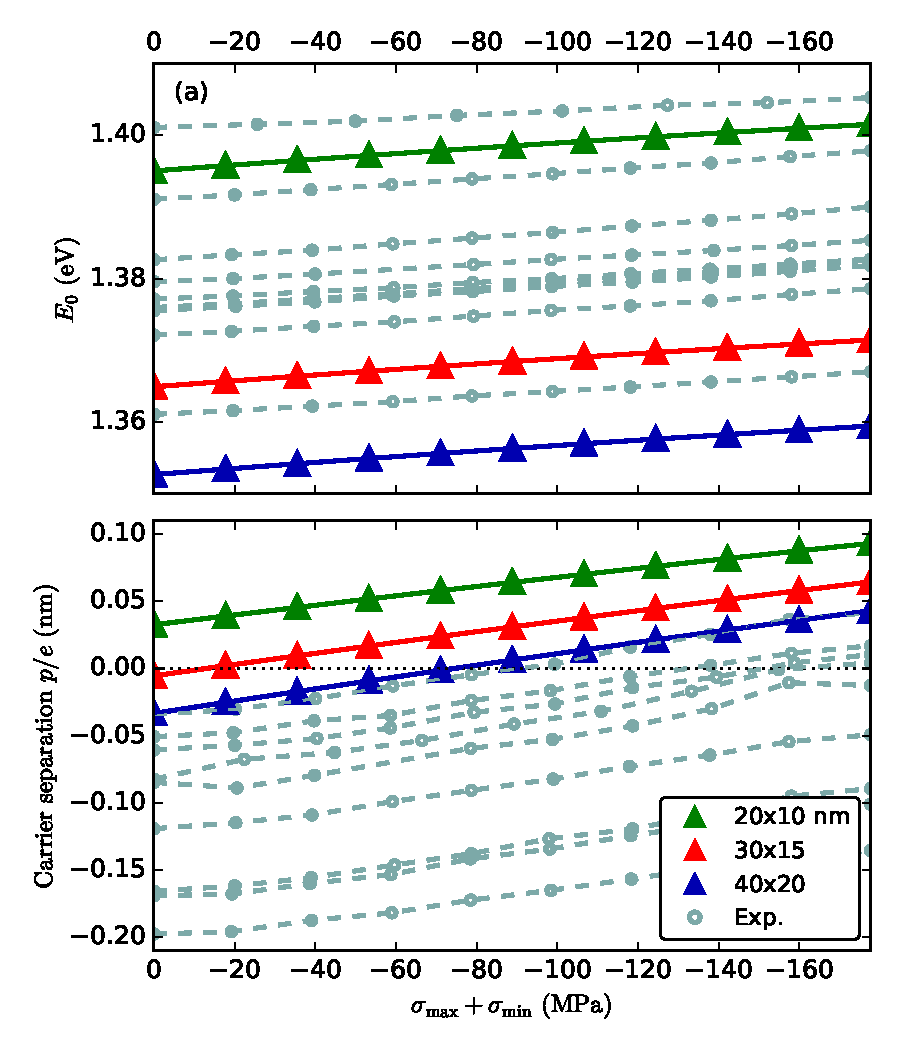
\includegraphics[width=0.5\textwidth]{/2_order/Energy/FINAL__171219_8x8_neotocena_++_nn+_35deg_pres350_h3___lateral} &
			%
			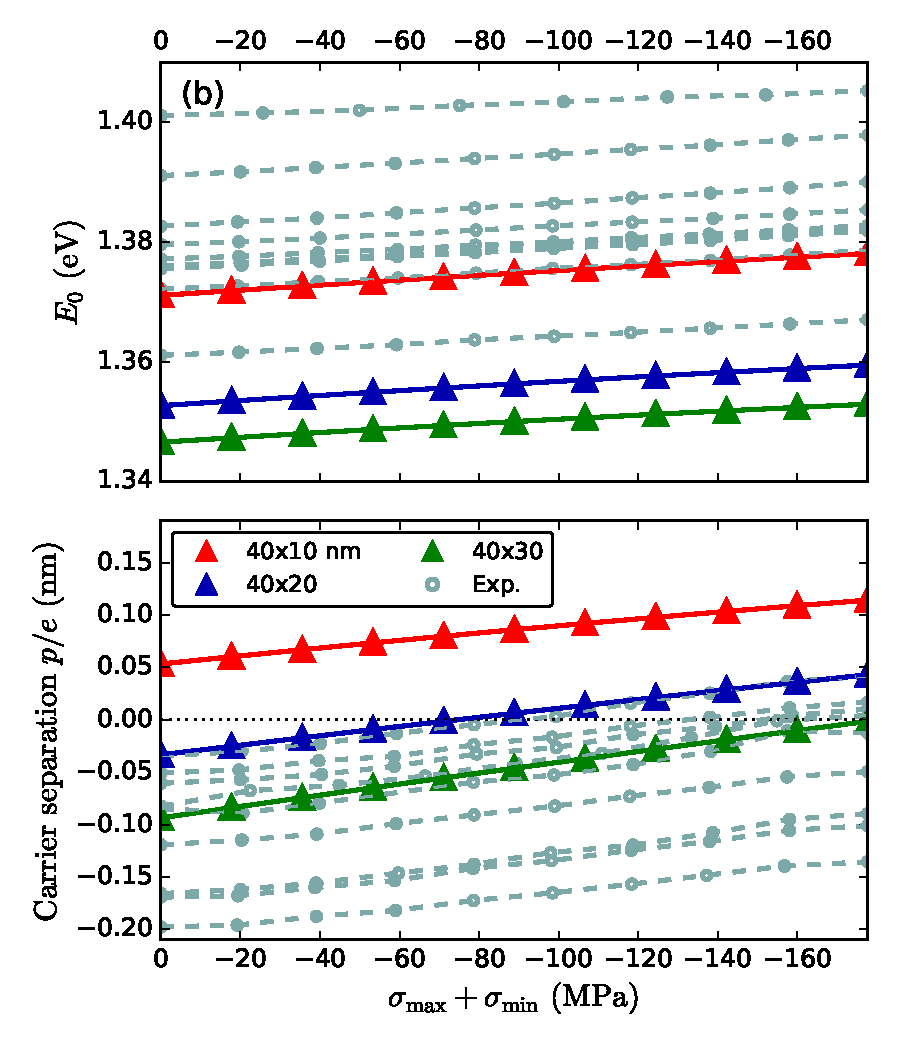
\includegraphics[width=0.5\textwidth]{/2_order/Energy/FINAL__171219_8x8_neotocena_++_nn+_35deg_pres350_h3___aspect} \\
		\end{tabular}
	\end{center}
	\caption{
		Dependencies of $E_0$ (top panels) and $p/e$ (bottom panels) on $\sigma_{\mathrm{max}}+\sigma_{\mathrm{min}}$ experimentally obtained from $\mu$PL measurements of nine InGaAs QDs~\cite{Aberl:17} (dashed curves) and that calculated for different values of (a) dot base diameter with fixed aspect ratio of 1/2 to the diameter of the the upper plane and (b) aspect with fixed base diameter of 40$\,$nm. Except for varied quantities the simulated QDs had the same properties as QD$_2$ including the value of $\sigma^{\mathrm{pre}}=350$$\,$MPa. The letter $e$ denotes the elementary charge.
		\label{fig:TuningByLateral}}
\end{figure}

Because previous analysis has led us to realize that only $\sigma^\mathrm{pre}$ and height are mostly important for tuning of $p$, we repeat similar evaluation as before,~i.~e., plot $A^\mathrm{QD}$ and $b$ as a function of QD height.
%
We can see in left column of Fig.~\ref{fig:FitHeightPrestress} that both $A^\mathrm{QD}$ and $b$ quadratically evolve with dot height. While $A^\mathrm{QD}$ shows similar dependence on height for all studied $\sigma^\mathrm{pre}$, dependence of $b$ on height is changing from convex for small $\sigma^\mathrm{pre}$ 
%(smaller than 500~MPa for QD$_2$) 
to concave for large values of $\sigma^\mathrm{pre}$. 

The latter behavior, in turn, provides comparison of the importance of dot structural properties particularly In alloy profile and $\sigma^{\mathrm{pre}}$ on $p$ for $\sigma_{\mathrm{max}}+\sigma_{\mathrm{min}}=0$. Smaller values of $\sigma^{\mathrm{pre}}$ are insufficient to overcome the effect of In alloy on dipole and, furthermore, for fixed value of $\sigma^{\mathrm{pre}}$ the influence of In alloy on dipole increases even more with QD height, leading to convex dependence. On the other hand, large values of $\sigma^{\mathrm{pre}}$ (in our structure $\sigma^{\mathrm{pre}}>500$$\,$MPa) rather easily overcome the effect of dot composition on dipole which is then mostly controlled only by $\sigma^{\mathrm{pre}}$.

%












\section*{Conclusions}
We have studied the effects of non-linear piezoelectricity on emission energy and electric dipole moment in stress tuned InGaAs/GaAs quantum dots and pinpointed the importance of that for studies of those systems as compared to using first-order terms only. 
%and pinpointed the dominant piezoelectric term. 
Also, we have shown the necessity of the presence of a large built-in in-plane strain due to the lattice mismatch in order for the pronounced changes of the electron-hole dipole to occur as a result of an externally applied stress. 

Furthermore, we have illustrated the use of an effective linear model to find the electric dipole moment in quantum dots as a function of quantum dot height and its build-in prestress. For these quantities we have shown the evolution of parameters from linear fits of the dipole on applied stress. 

Finally in Tab.~\ref{tab:conclusion_straintuned}, we summarize effects of selected parameters on emission energy and electric dipole.

\begin{table*}[ht!]
	\begin{center}
		\caption{Summary of different parameters that we used to tune the emission energy $E_0$ and electric dipole $p$ on the hydrostatic applied stress $\sigma^{\rm{app}}=\sigma_{\mathrm{max}}+\sigma_{\mathrm{min}}$ in stress-tuned InGaAs QDs assuming second-order piezoelectricity. Meaning of symbols is the following: symbol $\textcolor{ps_green}{\boldsymbol{+}}$ ($\textcolor{red}{\boldsymbol{-}}$) indicates increase (decrease) of $E_0$ or $p$ with increasing parameter in the leftmost column.  \label{tab:conclusion_straintuned} 
		}
		\begin{tabular}{c|cc|cc}
			\hline \hline
			\multirow{2}{*}{Dependency on} &  \multicolumn{2}{c|}{Energy} & \multicolumn{2}{c}{Dipole}\\ \cline{2-5}
			 &   $E_0$ & $\partial E_0/\partial\sigma_\mathrm{app}$  & $b$ & $A^{\mathrm{QD}}$\\  \hline
			 %
			 %
			 %2$^\mathrm{nd}$ piezo&   o & $\textcolor{ps_green}{\boldsymbol{+}}$  & o&$\textcolor{red}{\boldsymbol{-}}$\\ \hline
			 %
			  In contribution &  mean & o  & mean &o\\ \hline
			 %
			 $\sigma^\mathrm{pre}$ &  o &  $\textcolor{ps_green}{\boldsymbol{+}}$  & $\textcolor{red}{\boldsymbol{--}}$ &$\textcolor{red}{\boldsymbol{-}}$\\ \hline
			 %
			 Height&  $\textcolor{ps_green}{\boldsymbol{++}}$&  o  & $\textcolor{ps_green}{\boldsymbol{+}}$ &$\textcolor{ps_green}{\boldsymbol{++}}$\\ \hline
			 %
			 Base &  $\textcolor{ps_green}{\boldsymbol{++}}$&  o   &$\textcolor{ps_green}{\boldsymbol{++}}$ & o\\ \hline
			 %
			 Aspect &  $\textcolor{ps_green}{\boldsymbol{++}}$&  o   &$\textcolor{ps_green}{\boldsymbol{++}}$ & o\\ \hline
			 %
			 %
			 %
			 \multicolumn{5}{c}{o no effect \qquad $\textcolor{ps_green}{\boldsymbol{+}}$ increase \qquad $\textcolor{red}{\boldsymbol{-}}$ decrease }\\
			\hline \hline
		\end{tabular}
	\end{center}
\end{table*}



%https://books.google.cz/books?id=DiFMPmXSsLUC&pg=SA6-PA15&lpg=SA6-PA15&dq=Varshni+1967&source=bl&ots=hBJXnBqrHH&sig=WuCbtLj6FUIWMr09BP1LkBR-2cc&hl=cs&sa=X&ved=0ahUKEwi5mPz5lL_ZAhUGEVAKHRiaAOIQ6AEIXDAH#v=onepage&q=Varshni%201967&f=false

\chapter{InGaAsSb/GaAs/GaP QDs for Flash memories}\label{chap:TUB_QD}

%The direct-band gap semiconductor InGaAs represents the basic of the active area of a multitude of commercial photonic devices
%Optical emitters are one of the key components of optoelectronics and photonics. Despite the considerable progress in light emitting technology in visible spectral range during the last decades, the implementation of efficient light emitters on silicon remains a challenge. 
Today's market of computer memories is divided mainly between two kinds of memories, i.~e., the dynamical random access memory (DRAM)~\citep{waser_2003} and the flash memory~\citep{Pavan_1997}. The DRAM is fast but volatile, which means that the information must be refreshed within every tens milliseconds. On the other hand flash memory is a non-volatile memory with a storage time of more than ten years without any power consumption, however, it suffers from a slow write time of several microseconds. Semiconductor memory community is seeking for a memory based on the advantages of both previous types, which would combine the fast write/read speed with long storage time. Different approaches toward that goal are studied at the moment, such as FeRAM, MRAM or PCRAM, etc.~\citep{Burr_IBM2008}.

One of the promising options to combine fast write speed and long storage time is the use of QD-Flash~\citep{Geller_APL2008_QDFlash}, a memory based on self-organized quantum dots (QDs) fabricated from III-V materials. These nano-objects can be prepared by Stranski-Krastanov growth mode and due to a variety of material band structure engineering its band-offsets and barriers can be tuned in contrast to the fixed SiO$_2$ barriers in the current Flash memories.\\
%
\indent Storage of information is always a non-equilibrium situation, which is lost after a certain time. In the QD-based memory this process is limited by certain time of thermal emission only. The storage time for various materials based on either electron~\citep{Anand_apl1995_elflash,Nowozin_2013_sum} or hole~\citep{GellerPRB, stracke_apl2012_qdflash_GaP,Nowozin_2013_sum} storages were studied. The energy levels of confined holes in a QD are much more favourably confined than those of electrons owing to their larger effective mass, therefore, at least one order of magnitude more holes can be stored in a given volume than electrons. \\
%
\indent One of the suitable systems for realization of long storage time QD-Flash are heterostructures grown on GaP substrate. For In$_{0.25}$Ga$_{0.75}$As/GaAs/GaP the storage time of 3~$\mu$s was measured at room temperature~\citep{stracke_apl2012_qdflash_GaP}, which is insufficient for memory usage, however, it is already three orders higher than the time for a typical representative of III-V QDs from InGa/GaAs~\citep{GellerPRB}. Longer storage time can be expected in the GaSb/GaP system, due to higher localization energy. Several pioneering studies have been reported for GaSb/GaP system, where the storage time is predicted in a range 1 and $10^5$ years with 8-band $\mathbf{k\cdot p}$ calculations~\citep{Bimberg_proceedingSPIE}, however the experimentally observed times were not larger than 3.9~days~\citep{Bonato_pssolidi_GaSbonGaP}.\\%  Moreover, the storage time for GaSb/GaP heterostructure was predicted in a range 1 and $10^5$ years with 8-band $\mathbf{k\cdot p}$ calculations~\citep{Bimberg_proceedingSPIE}.\\
%
\indent The use of structures grown on GaP substrate has another benefit besides other III-V semiconductors, where crystalline defects are generated during the III-V/Si heteroepitaxy. It was proposed to use pseudomorphic GaP/Si substrate benefiting from the low lattice mismatch between GaP and Si (0.37~\% at 300~K) to avert the formation of these defects~\citep{Beyer_jap2013,Grassman_apl2013, Lin_jcg2013}. Hence, the GaP-based heterostructures can be implemented in defect-free quality on Si chips.

In this chapter, we follow several previous experimental works which investigated {(In,Ga)As/GaP} QDs. InAs/GaP QDs have first been reported in Refs.~\citep{Leon_apl1998, guo_solidi2009}, but efficient PL was not achieved because of the plastic relaxation due to the large lattice mismatch (11.2\%). Then Futchi et al.~\citep{Fuchi_physicaE2004} measured PL up to 77~K on InGaAs/GaP QDs and pointed to the issue of In composition and dominant role of In amount was demonstrated via calculations~\citep{Fukami_solodi2011}. Rivoire et al.~\citep{Rivoire_prb2012} claimed a single dot emission of type-I In$_{0.5}$Ga$_{0.5}$As/GaP QDs, subsequently, the structural and emission properties were studied~\cite{Stracke_apl2014, Sala_apl2016}. To initiate the Stranski-Krastanov growth mode of In$_x$Ga$_{1-x}$As QDs on GaP, the GaP surfaces need to be covered by thin layer of GaAs prior to In$_x$Ga$_{1-x}$As deposition~\citep{stracke_apl2012_qdflash_GaP}.
%
%
% konec korekci PK
%
%
We investigate a set of samples with In$_{1-x}$Ga$_{x}$As$_y$Sb$_{1-y}$/GaAs/GaP QDs with GaAs thickness of 5~ML by centered around the energy of 1.8~eV, where emission from QDs is expected. We study PL of these samples as function of excitation power and temperature. The dynamics of optical transitions in the studied ensemble is examined by time-resolved PL (TRPL).


\section{In$_{1-x}$Ga$_{x}$As$_y$Sb$_{1-y}$/GaAs/GaP QDs samples}
The samples were grown on GaP(001) substrate by metalorganic vapor phase epitaxy (MOVPE) in Stranski-Krastanov mode in a horizontal Aixton 200 reactor using H$_2$ as carrier gas at Technische Universität Berlin~\citep{Sala_apl2016}. \\
%
\indent The growth starts with 250~nm GaP buffer layer followed by 20~nm AlGaP barrier and 150~nm GaP at the temperature of 750~$^\circ$C. Subsequently the temperature is reduced to 500~$^\circ$C for the following steps: (i) growth of a thin GaAs interlayer (5~ML) for all studied samples, (ii) for samples which we call S$_\mathrm{with}$ and S$_\mathrm{cap}$ a short Sb-flush is applied by supplying the triethyl-antimony for two and one second, respectively, at input flux of $2.6~\mu\mathrm{mol/min}$, (iii) In$_{1-x}$Ga$_{x}$As$_y$Sb$_{1-y}$ QDs growth, (iv) GaSb cap in case of sample S$_\mathrm{cap}$ (v) growth interruptions (GRI) for 1~s, and finishing the structure by GaP capping layer of 6~nm thickness. Finally, samples are heated to 620~$^\circ$C to grow 50~nm thick GaP layer. The samples are depicted in Fig.~\ref{fig:TUstructure} and their differences and labels are summarized in Tab.~\ref{tab:samples}.
\begin{figure}
	\centering
	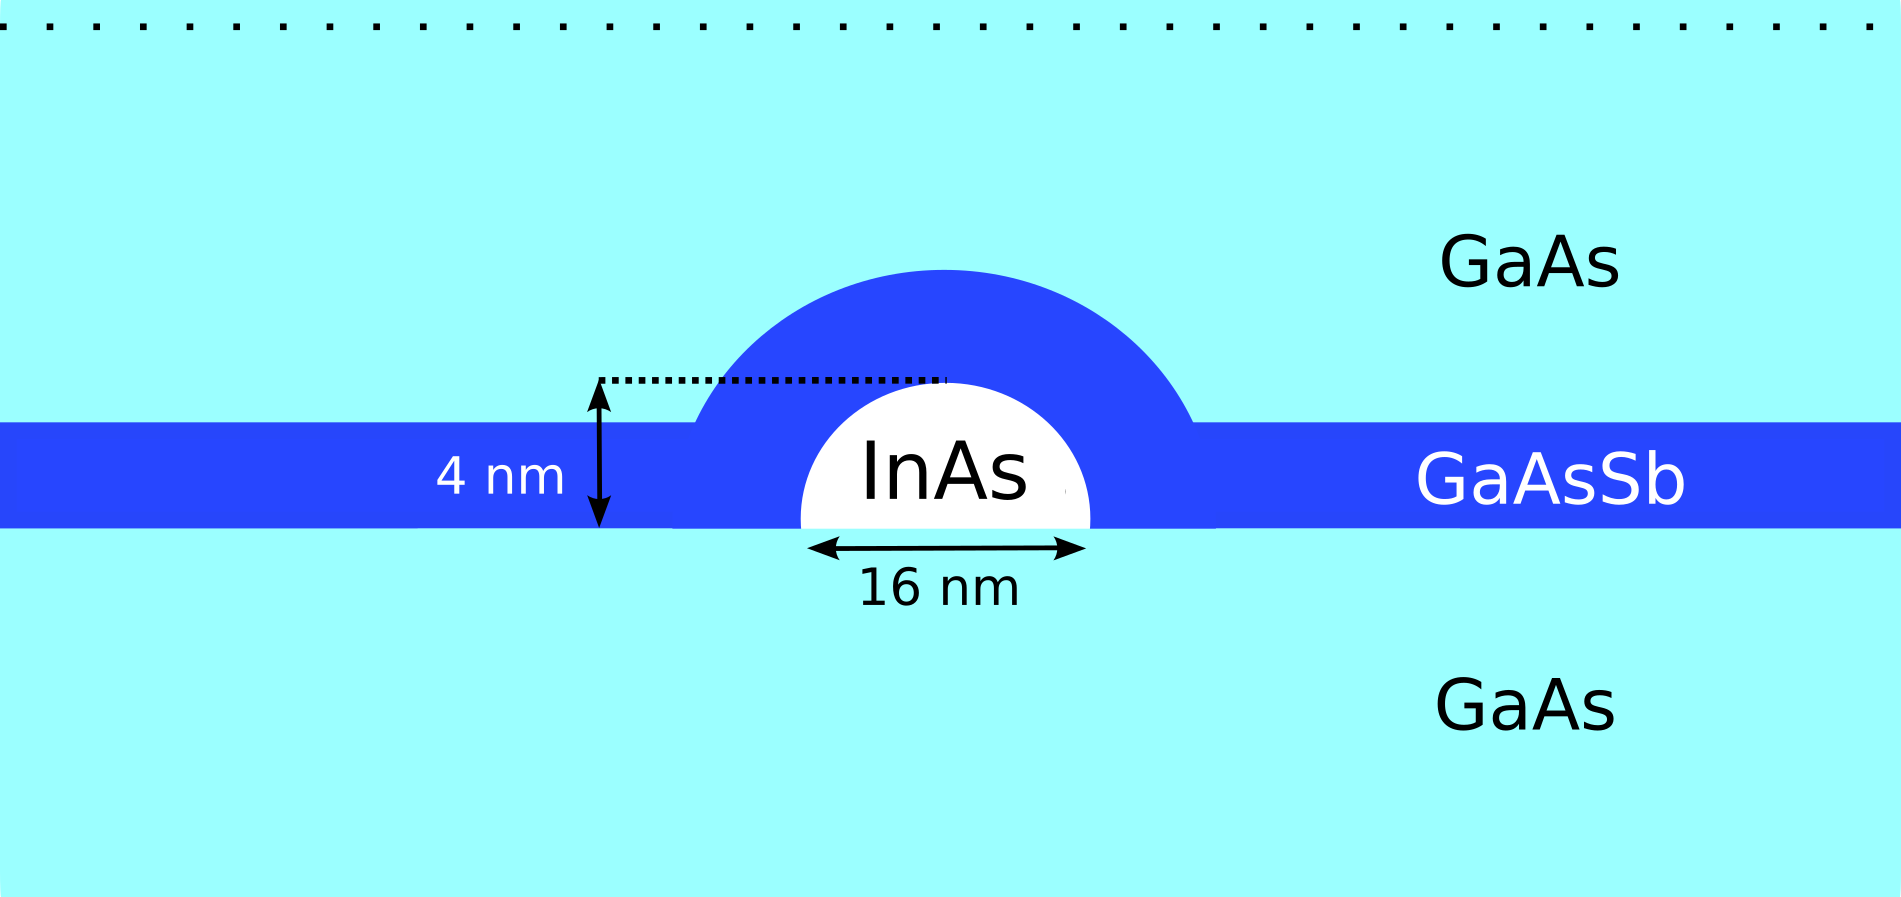
\includegraphics[width=1\linewidth]{/TEM/structure}
	\caption{Studied set of samples, $S_\mathrm{w/o}$ represents structure without QDs, $S_\mathrm{with}$ and $S_\mathrm{cap}$ are samples with In$_{1-x}$Ga$_{x}$As$_y$Sb$_{1-y}$ QDs, $S_\mathrm{cap}$ is, moreover, GaSb capped. }
	\label{fig:TUstructure}
\end{figure}

\begin{table}
	\centering
	\caption{Labels and studied sample differences.}
	%\begin{tabularx}{0.9\textwidth}{ccccc}
	\begin{tabularx}{0.95\textwidth}{ccl}
		\toprule

		%growing name & our marking& \multicolumn{3}{c}{specification}\\ 
		sample name & label& \multicolumn{1}{c}{specification}\\ 		
		\midrule
		\midrule
		%TU 12027& $S_\mathrm{w/o}$ & 5ML GaAs& &\\
		TU 12027& S$_\mathrm{w/o}$ & 5ML GaAs\\
		%TU 12040& $S_\mathrm{with}$ & 5ML GaAs,& 0.51ML In$_{1-x}$Ga$_{x}$As$_y$Sb$_{1-y}$&\\
		TU 12040& S$_\mathrm{with}$ & 5ML GaAs, 0.51~ML In$_{1-x}$Ga$_{x}$As$_y$Sb$_{1-y}$ QDs\\
		%TU 12021 & $S_\mathrm{cap}$ & 5ML GaAs,& 0.51ML In$_{1-x}$Ga$_{x}$As$_y$Sb$_{1-y}$,& GaSb cap\\
		TU 12021 & S$_\mathrm{cap}$ & 5ML GaAs, 0.51~ML In$_{1-x}$Ga$_{x}$As$_y$Sb$_{1-y}$ QDs, GaSb cap\\
		\bottomrule
	\end{tabularx}\label{tab:samples}
\end{table}

% http://nano.ceitec.cz/high-resolution-scanning-transmission-electron-microscope-fei-titan-themis-60-300-cubed/

We have studied the material composition of the sample S$_\mathrm{cap}$ by transmission electronic microscopy (TEM) with an add-on energy-dispersive X-ray (EDX) detector (SUPER-X EDX detector was used). These measurements were performed at the high resolution TEM FEI Titan Themis at CEITEC Brno. The TEM image of the whole sample and EDX emission spectrum are attached in appendix~\ref{chapter:appendix_TEM}.

In Fig.~\ref{fig:TEM}, cross-sectional TEM micrograph and graphs from parallel measured EDX for sample S$_\mathrm{cap}$ are presented. EDX spectrum is collected along the orange dashed line and averaged in the yellow boundary area. In the atomic fraction graph we show material composition in the sample as a function of horizontal position for all constituents (Ga, P, As, In, Sb). In the range between 30 and 40~nm in the cut In, As and Sb composition (elements, which are expected only in QDs area) dramatically in comparison with the concentration of 0.8~\% seen in the remainder of the sample. In the same range, we can see a decrease in phosphorus concentration at the expense of GaP. The layer where In concentration is higher than 0.8~\% we regard as QD area and its thickness is found to be of 5.8~nm with truncated-pyramid shape QDs with a base length of about 15~nm and a height of 2.5~nm. 
\begin{figure}
	\centering
	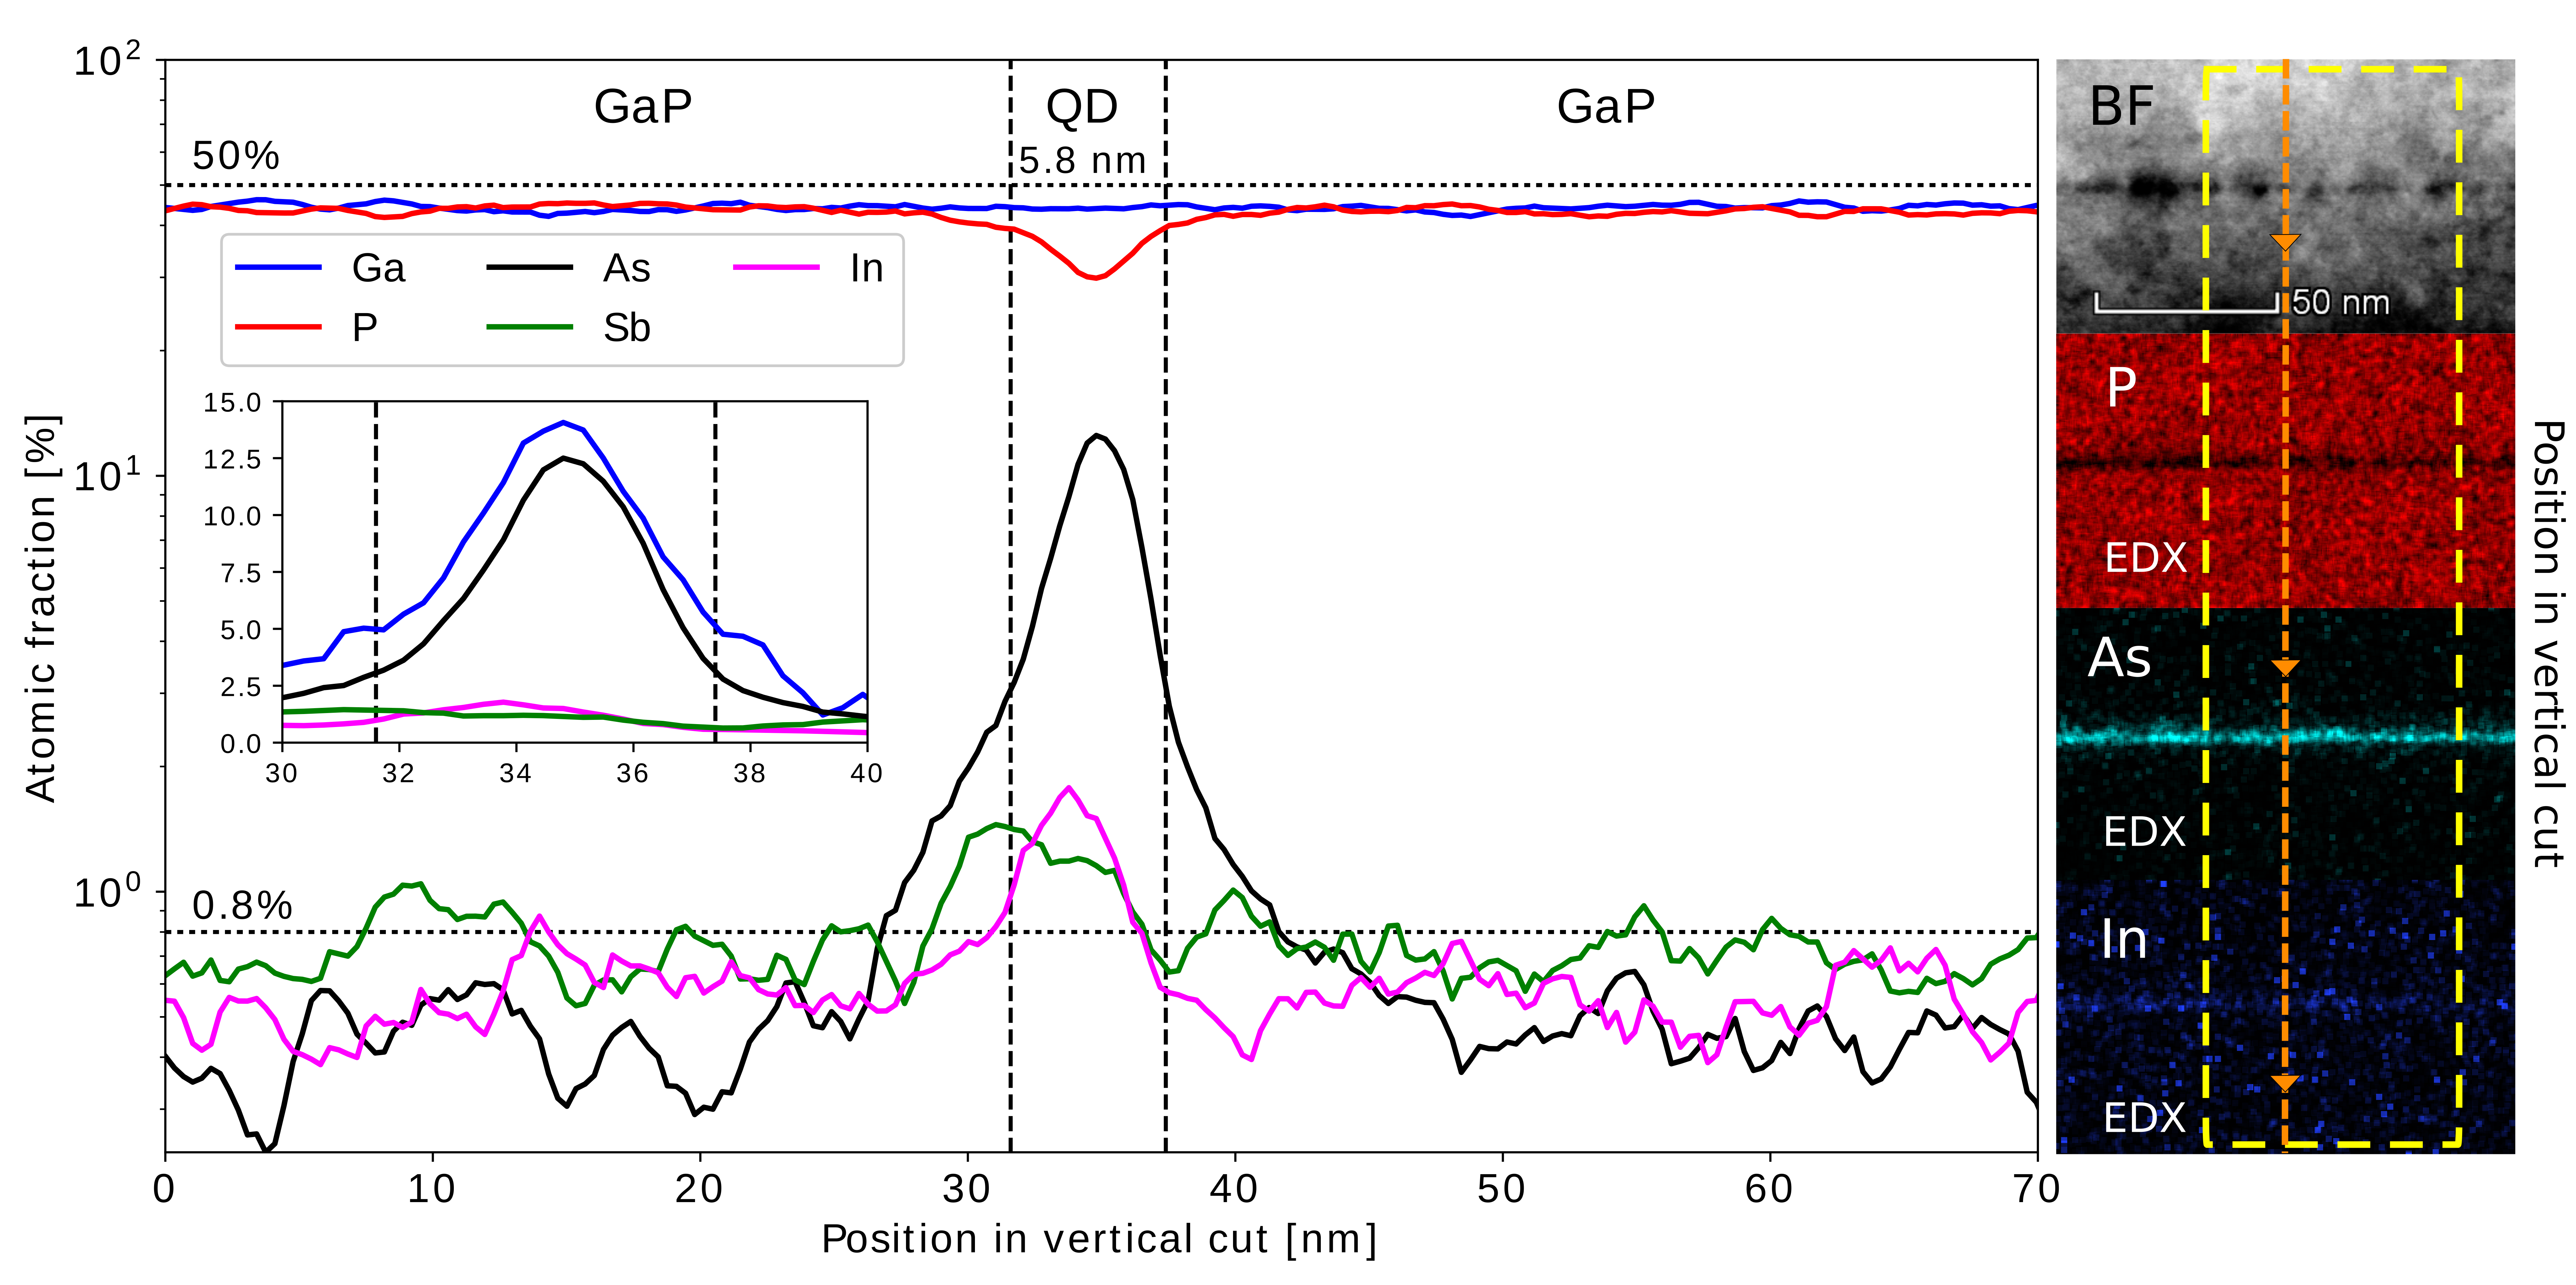
\includegraphics[width=1\linewidth]{/TEM/koncentrace_final_mapa2_QDinset}
	\caption{The atomic fraction vs. position in the vertical cut for all elements present in sample S$_\mathrm{cap}$ measured by EDX detector along the orange line in the right panel and averaged in the area circumferenced by the yellow broken curve. In QD area, i.~e., between the vertical positions of 30 and 40~nm in the cut, a substantial increase of In, As, Sb (compounds only in QD structures) and decrease of P (P is out of the QD structures) are observed. The inset shows the composition solely in the QD region. The column on right-hand side represents from top to bottom: cross-section TEM image of S$_\mathrm{cap}$ taken under strong-beam bright field condition using the (200) reflection perpendicular to the growth direction; and three EDX images measured at the same time as TEM measurements -- red one for P, white in As and purple in In.}
	\label{fig:TEM}
\end{figure}

We use the EDX data to estimate the concentration of individual elements in quaternary QD structure. Assuming that all phosphorus is bound in GaP, the concentration of Ga can be deconvoluted into Ga concentration in GaP $C_\mathrm{GaP}$ and in QD area $C_\mathrm{Ga}^\mathrm{QD}$ as
%
\begin{eqnarray}
C_\mathrm{Ga}=C_\mathrm{GaP}+C_\mathrm{Ga}^\mathrm{QD}=C_\mathrm{P}+C_\mathrm{Ga}^\mathrm{QD},
\end{eqnarray}
%
where $C_\mathrm{i}$ for $i \in \{\mathrm{Ga}, \mathrm{P}\}$ is the measured concentration of Ga and P. We assume the composition of our QDs in the form of In$_{1-x}$Ga$_{x}$As$_y$Sb$_{1-y}$, thus, we can calculate effective concetration in QD area as
%
\begin{eqnarray}
x=\frac{C_\mathrm{Ga}^\mathrm{QD}}{C_\mathrm{Ga}^\mathrm{QD}+C_\mathrm{In}^\mathrm{QD}},\qquad
y=\frac{C_\mathrm{As}^\mathrm{QD}}{C_\mathrm{As}^\mathrm{QD}+C_\mathrm{Sb}^\mathrm{QD}}.
\end{eqnarray}
%
Given the assumption that In, Ga and Sb are only in QD area, we can replace the concentration in this region with directly measured concentration by EDX. Finally, we give the estimation of $x$ and $y$ which we use in 8-band $\mathbf{k\cdot p}$ calculations of $x=84-93.5~\%$ and $y=68-91.5~\%$, see Fig.~\ref{fig:concentration_estimation}.


\begin{figure}
	\centering
	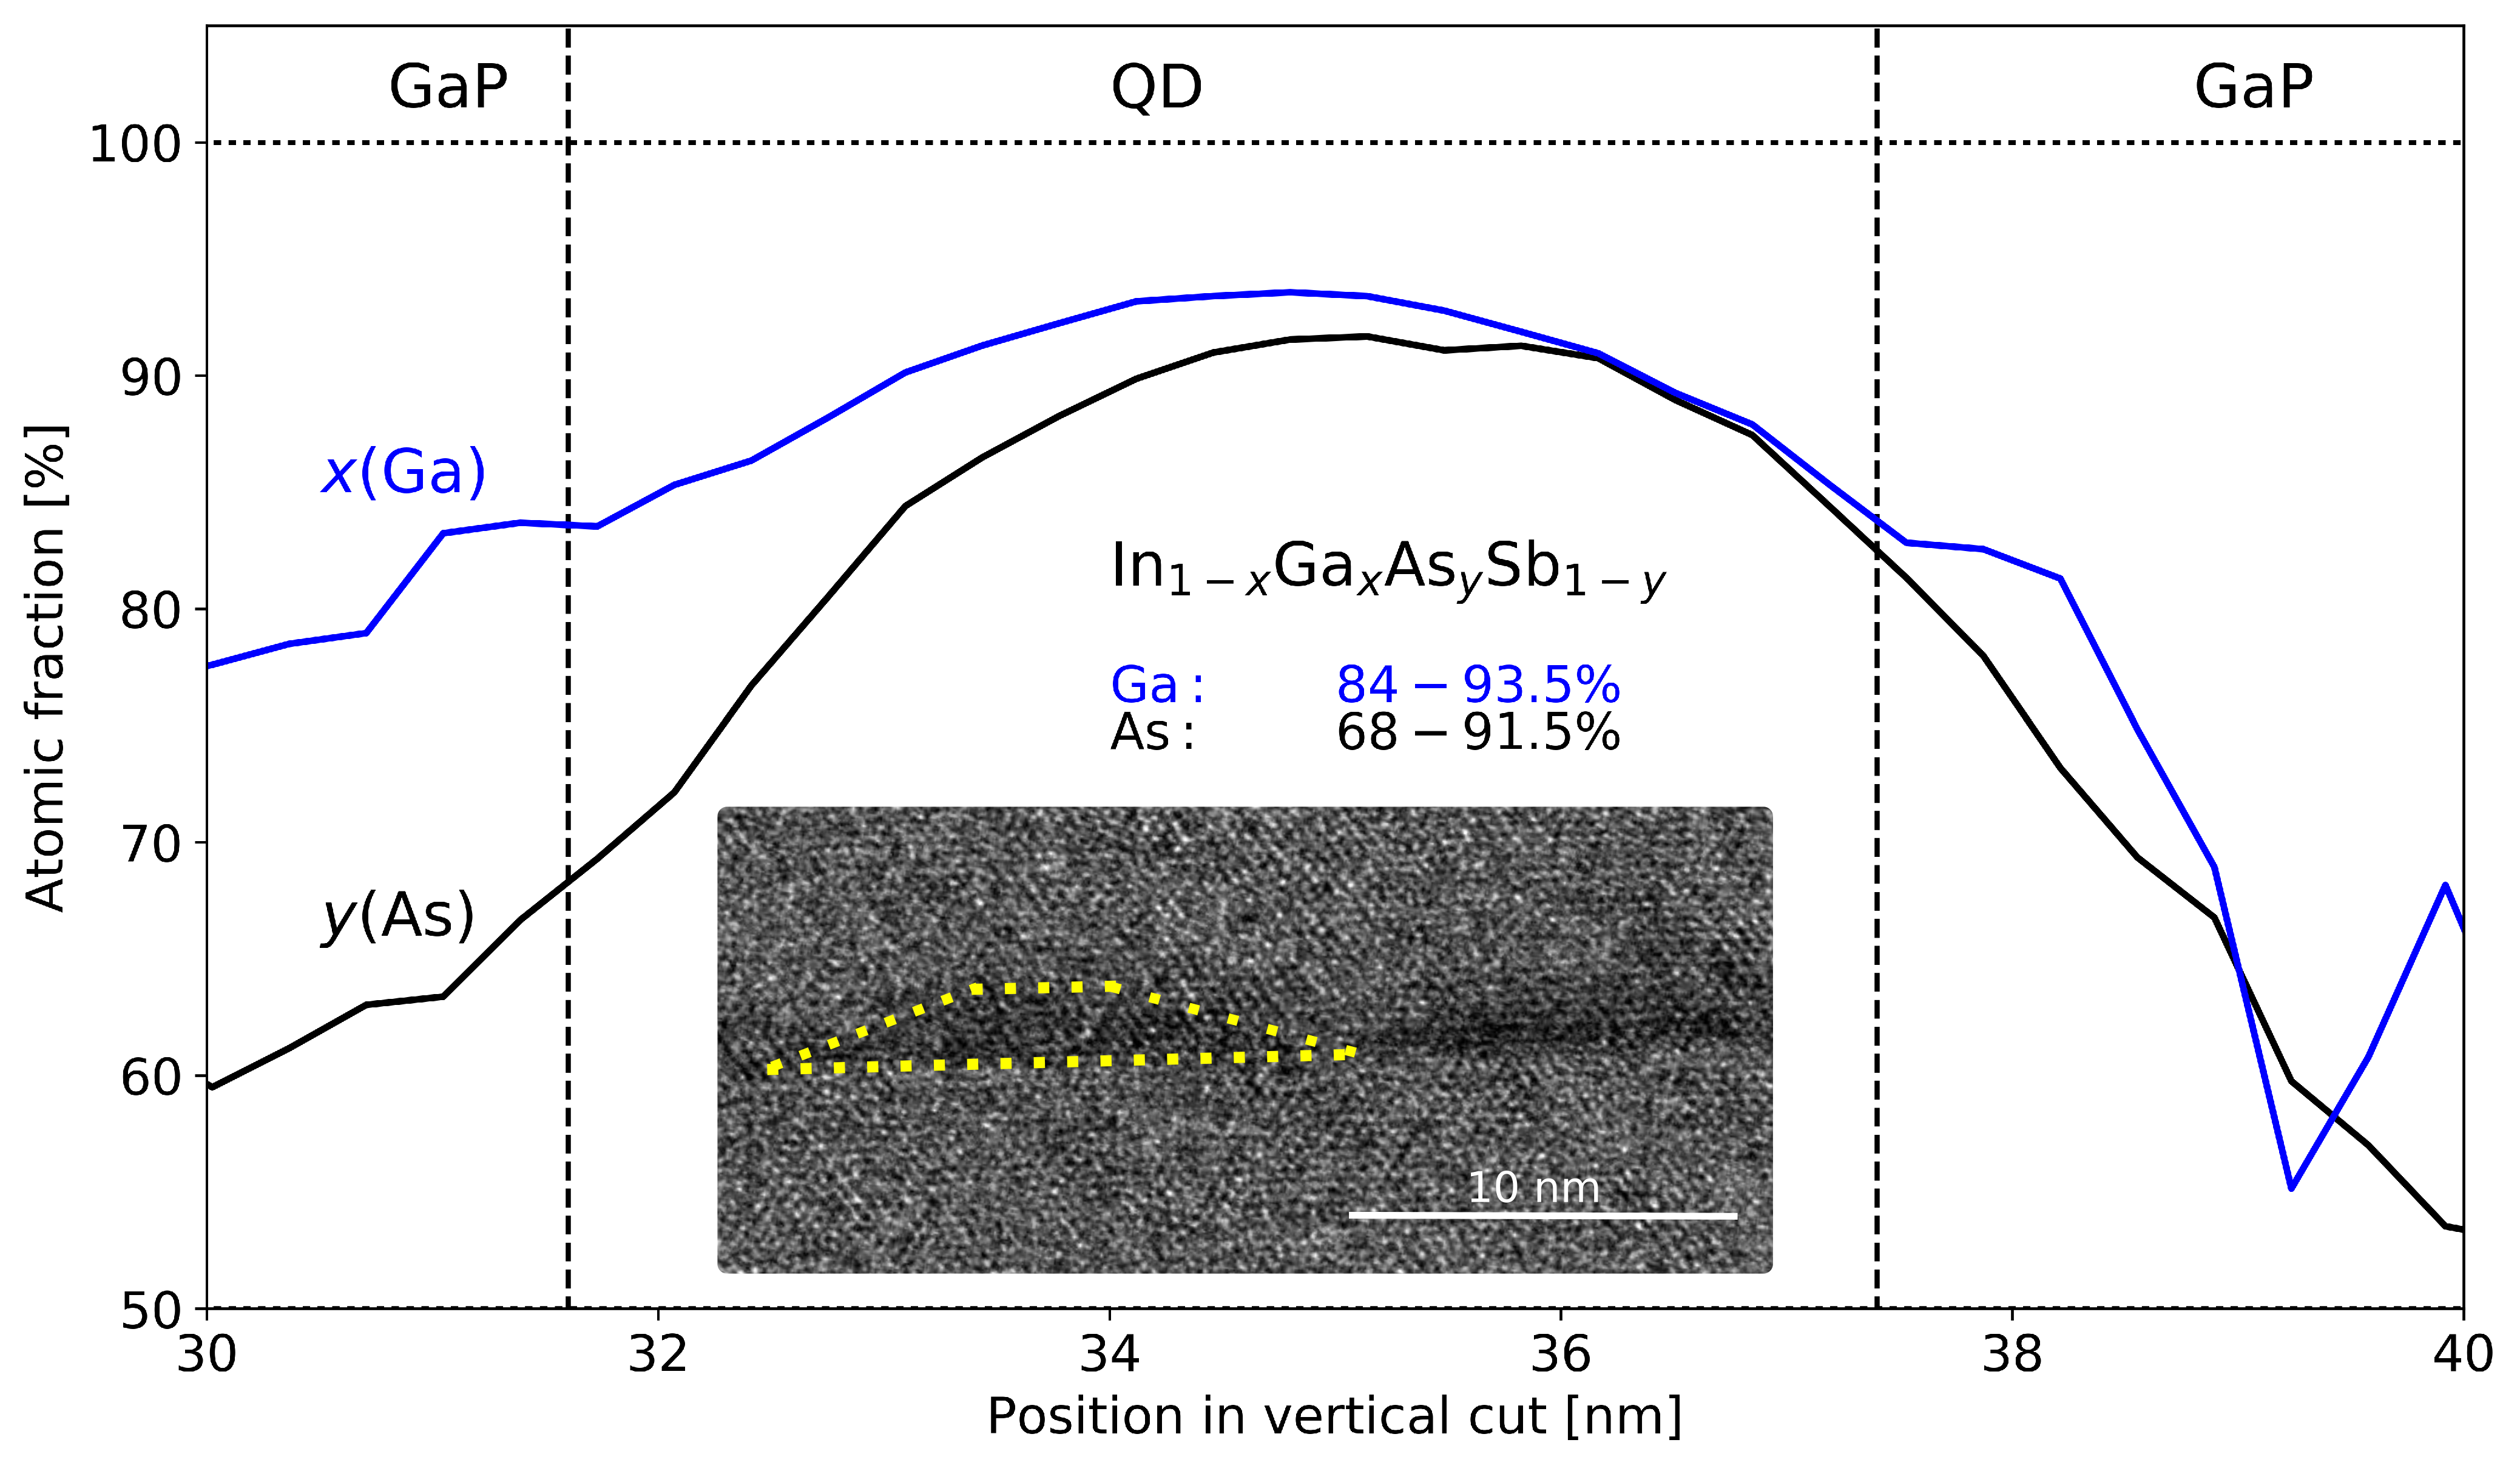
\includegraphics[width=0.85\linewidth]{/TEM/koncentrace_pro_nn} %rez_QD_konc_xy_bez}
	\caption{The estimated composition of QD area for sample S$_\mathrm{cap}$. We assume Ga and As concentration to be in the ranges of 84-93.5~\% and 68-91.5~\%, respectively. In inset we show the HRTEM image of a truncated-pyramid QD.}
	\label{fig:concentration_estimation}
\end{figure}

\clearpage

\section{Estimation of hydrostatic strain in GaAs layer}
For estimation of a hydrostatic component of the strain was performed room temperature Raman measurements of our samples. These measurements were obtained using NT-MDT spectrometer with a 100$\times$/0.7~NA long working length objective and the 532~nm laser. The scattered light was dispersed using a 1800~groove/mm grating and detected by a thermoelectrically cooled Si CCD camera. The spectra were recorded in $z(xy)z$ backscattering geometry.

Measured signals were fitted by the sum of 3 Lorentzian curves.
Let we focus to Raman signal around 290~cm$^{-1}$ where the TO phonon of strained GaAs QWs for our QDs samples is expected. Fig.~\ref{fig:raman} reports about $\sim$19~cm$^{-1}$ shift of TO phonon for our QDs samples compared to bulk material. Using a model~\cite{Montazeri_Nano2010}, we can use the shift to estimate the value of hydrostatic strain $\epsilon_{xx}$ 
\begin{equation}
k_\mathrm{TO}^2 = k_\mathrm{TO,B}^2 + (p+2q)\epsilon_{xx},
\end{equation}
where $k_\mathrm{TO}$ and $k_\mathrm{TO,B}$ are the Raman shifts of TO GaAs mode of strained and bulk GaAs, and $p$ and $q$ are phonon deformation potentials taken from Ref.~\cite{Cerdeira_PRB1972}.

The measured shifts of TO mode of $S_\mathrm{w/o}$ correspond to $\epsilon_{xx}=-0.032$, of $S_\mathrm{with}$ to $\epsilon_{xx}=-0.026$,  and for $S_\mathrm{cap}$ is $\epsilon_{xx}=-0.030$, which is in good agreement with the predicted hydrostatic strain component $\epsilon_{xx}=-0.034$ by the $\mathbf{k \cdot p}$ calculations, see Fig.~\ref{fig:raman_theory_wo}. %approximately three times less than predicted hydrostatic strain component by the $\mathbf{k \cdot p}$ calculations, see Fig.~\ref{fig:raman_theory_wo}.
\begin{figure}
	\centering
	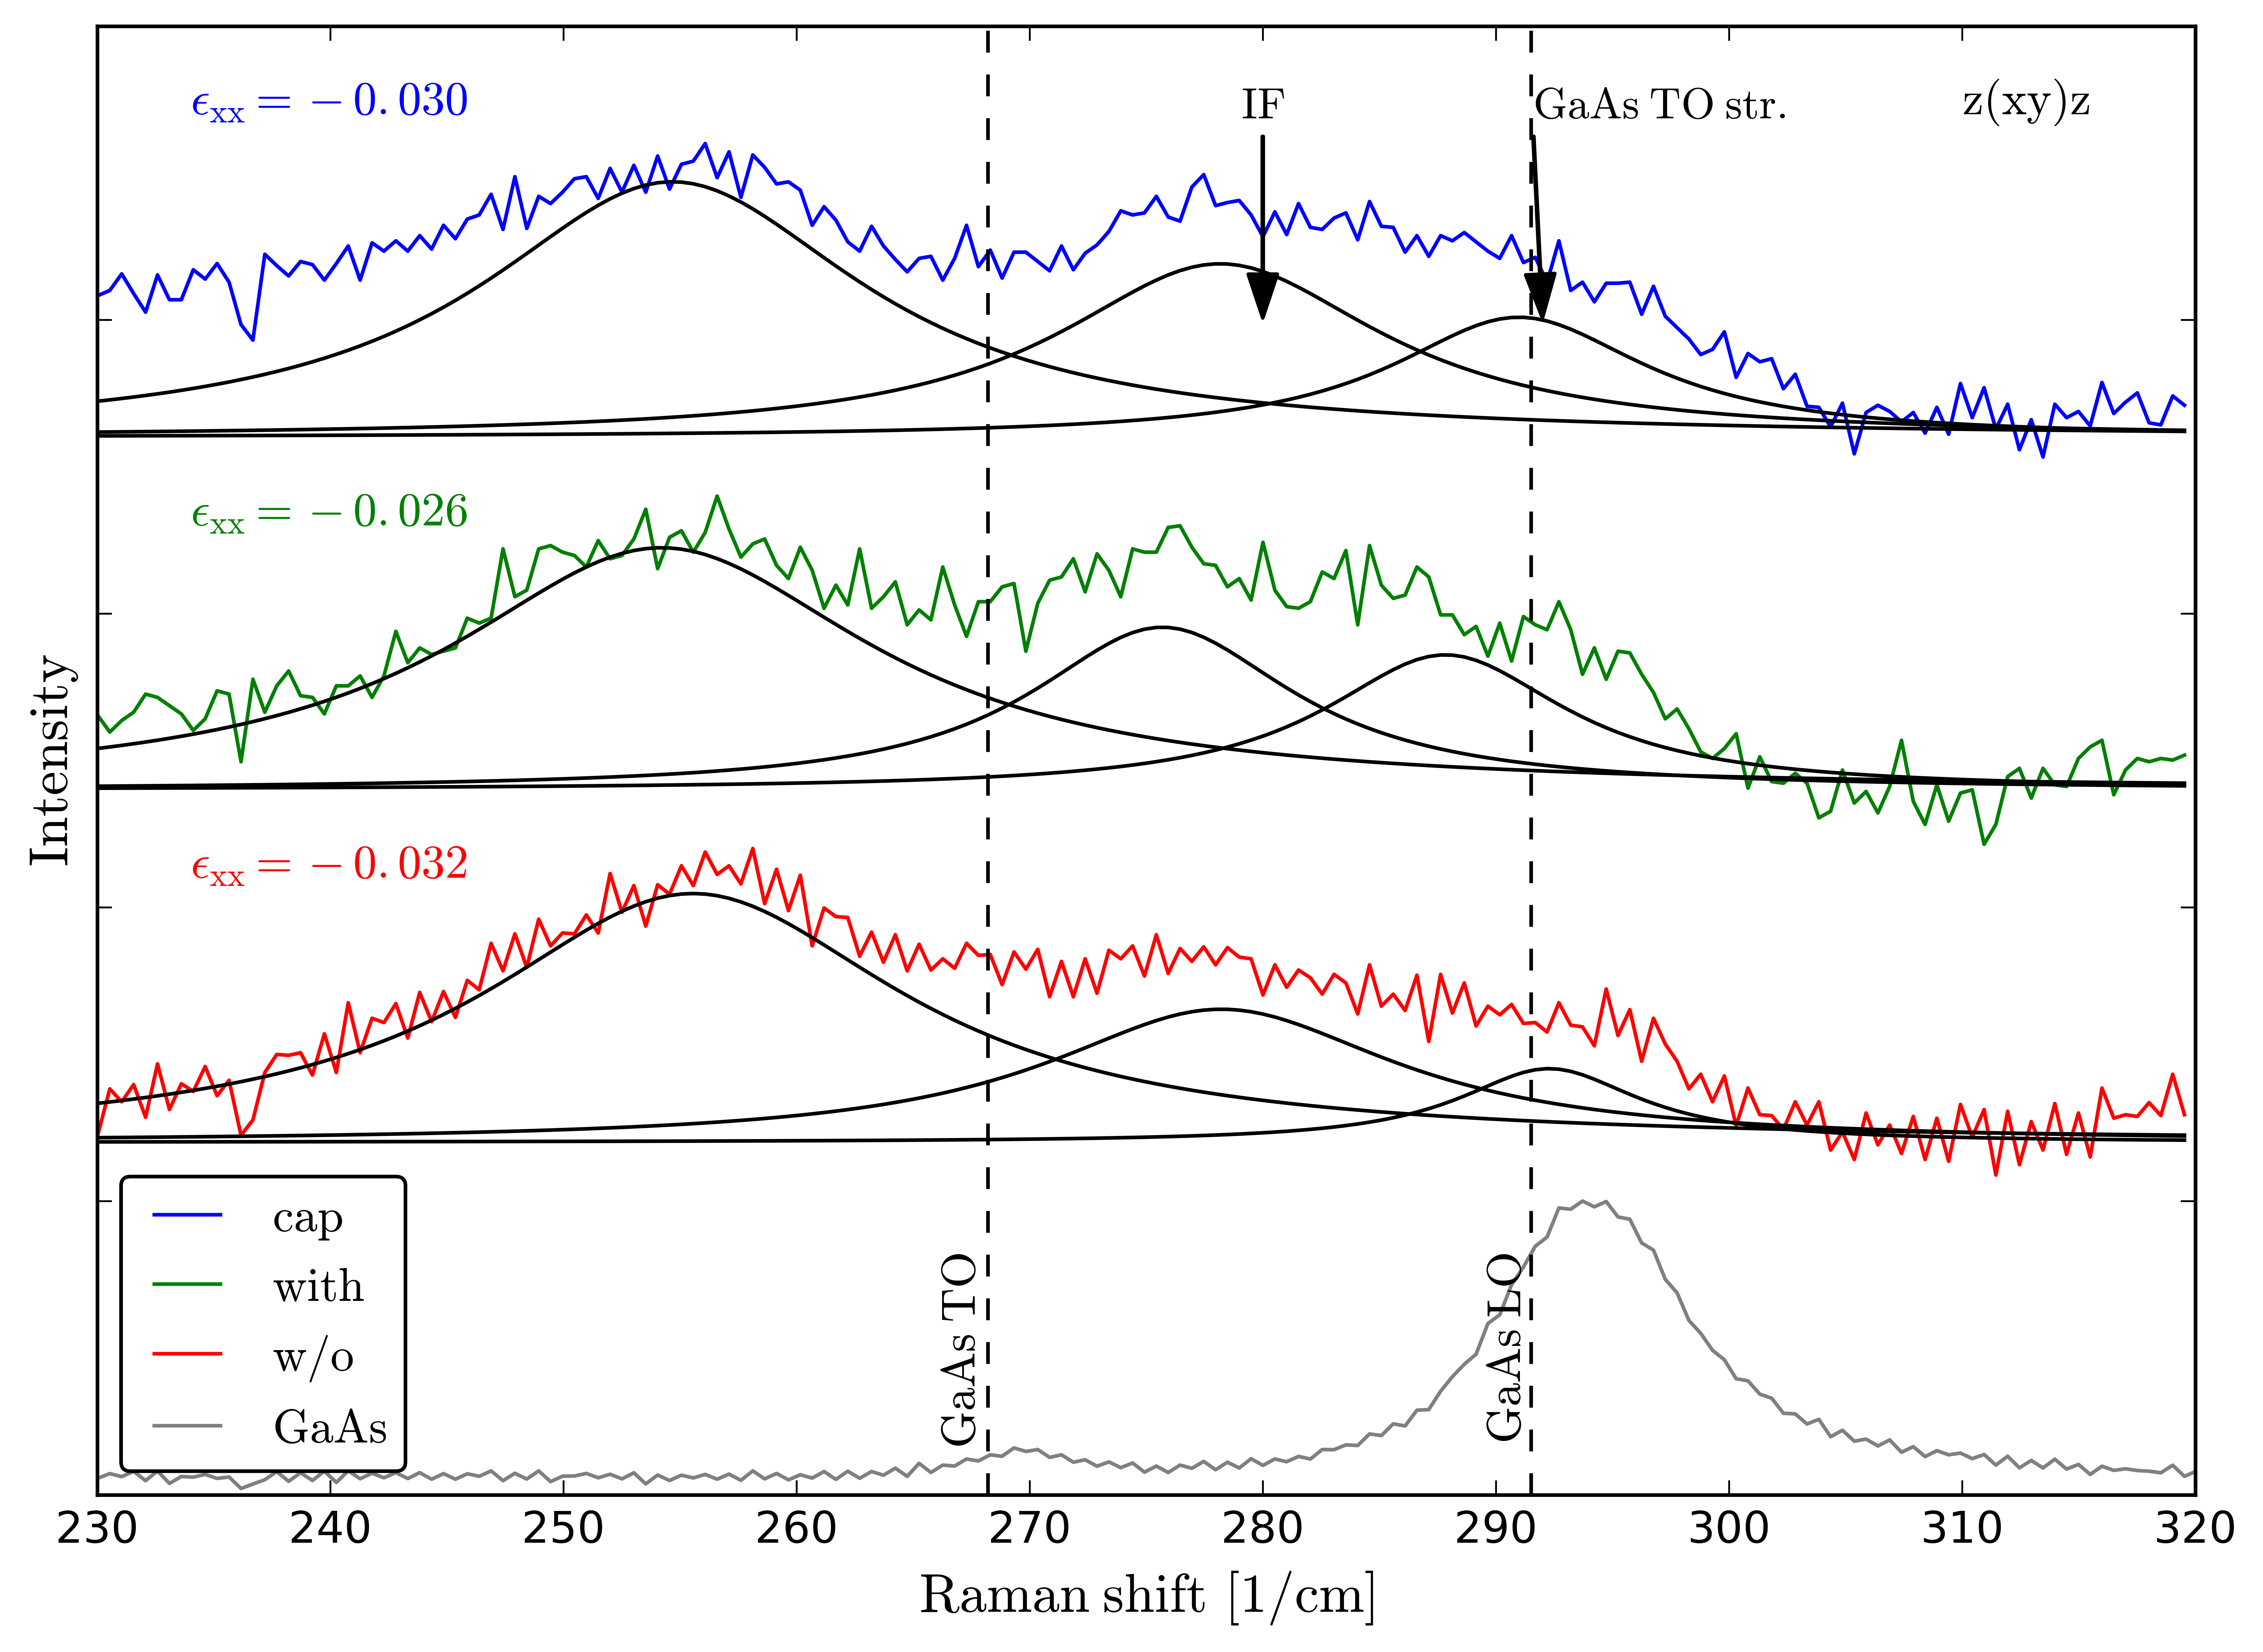
\includegraphics[width=0.85\linewidth]{/raman/Raman_TUB_and_GaAs_enlg_230_to_320_fit}
	\caption{Raman spectra of samples w/o QDs $S_\mathrm{w/o}$ (red), with QDs $S_\mathrm{with}$ (green) and capped QDs $S_\mathrm{cap}$ and bulk GaAs (grey). The dashed lines show reference GaAs TO and LO modes~\citep{Esther_Nanotech2013}. Calculated hydrostatic strain components $\epsilon_{xx}$ are presented in inset of the figure. A label IF corresponds to interface Raman band.}
	\label{fig:raman}
\end{figure}

\begin{figure}
	\centering
	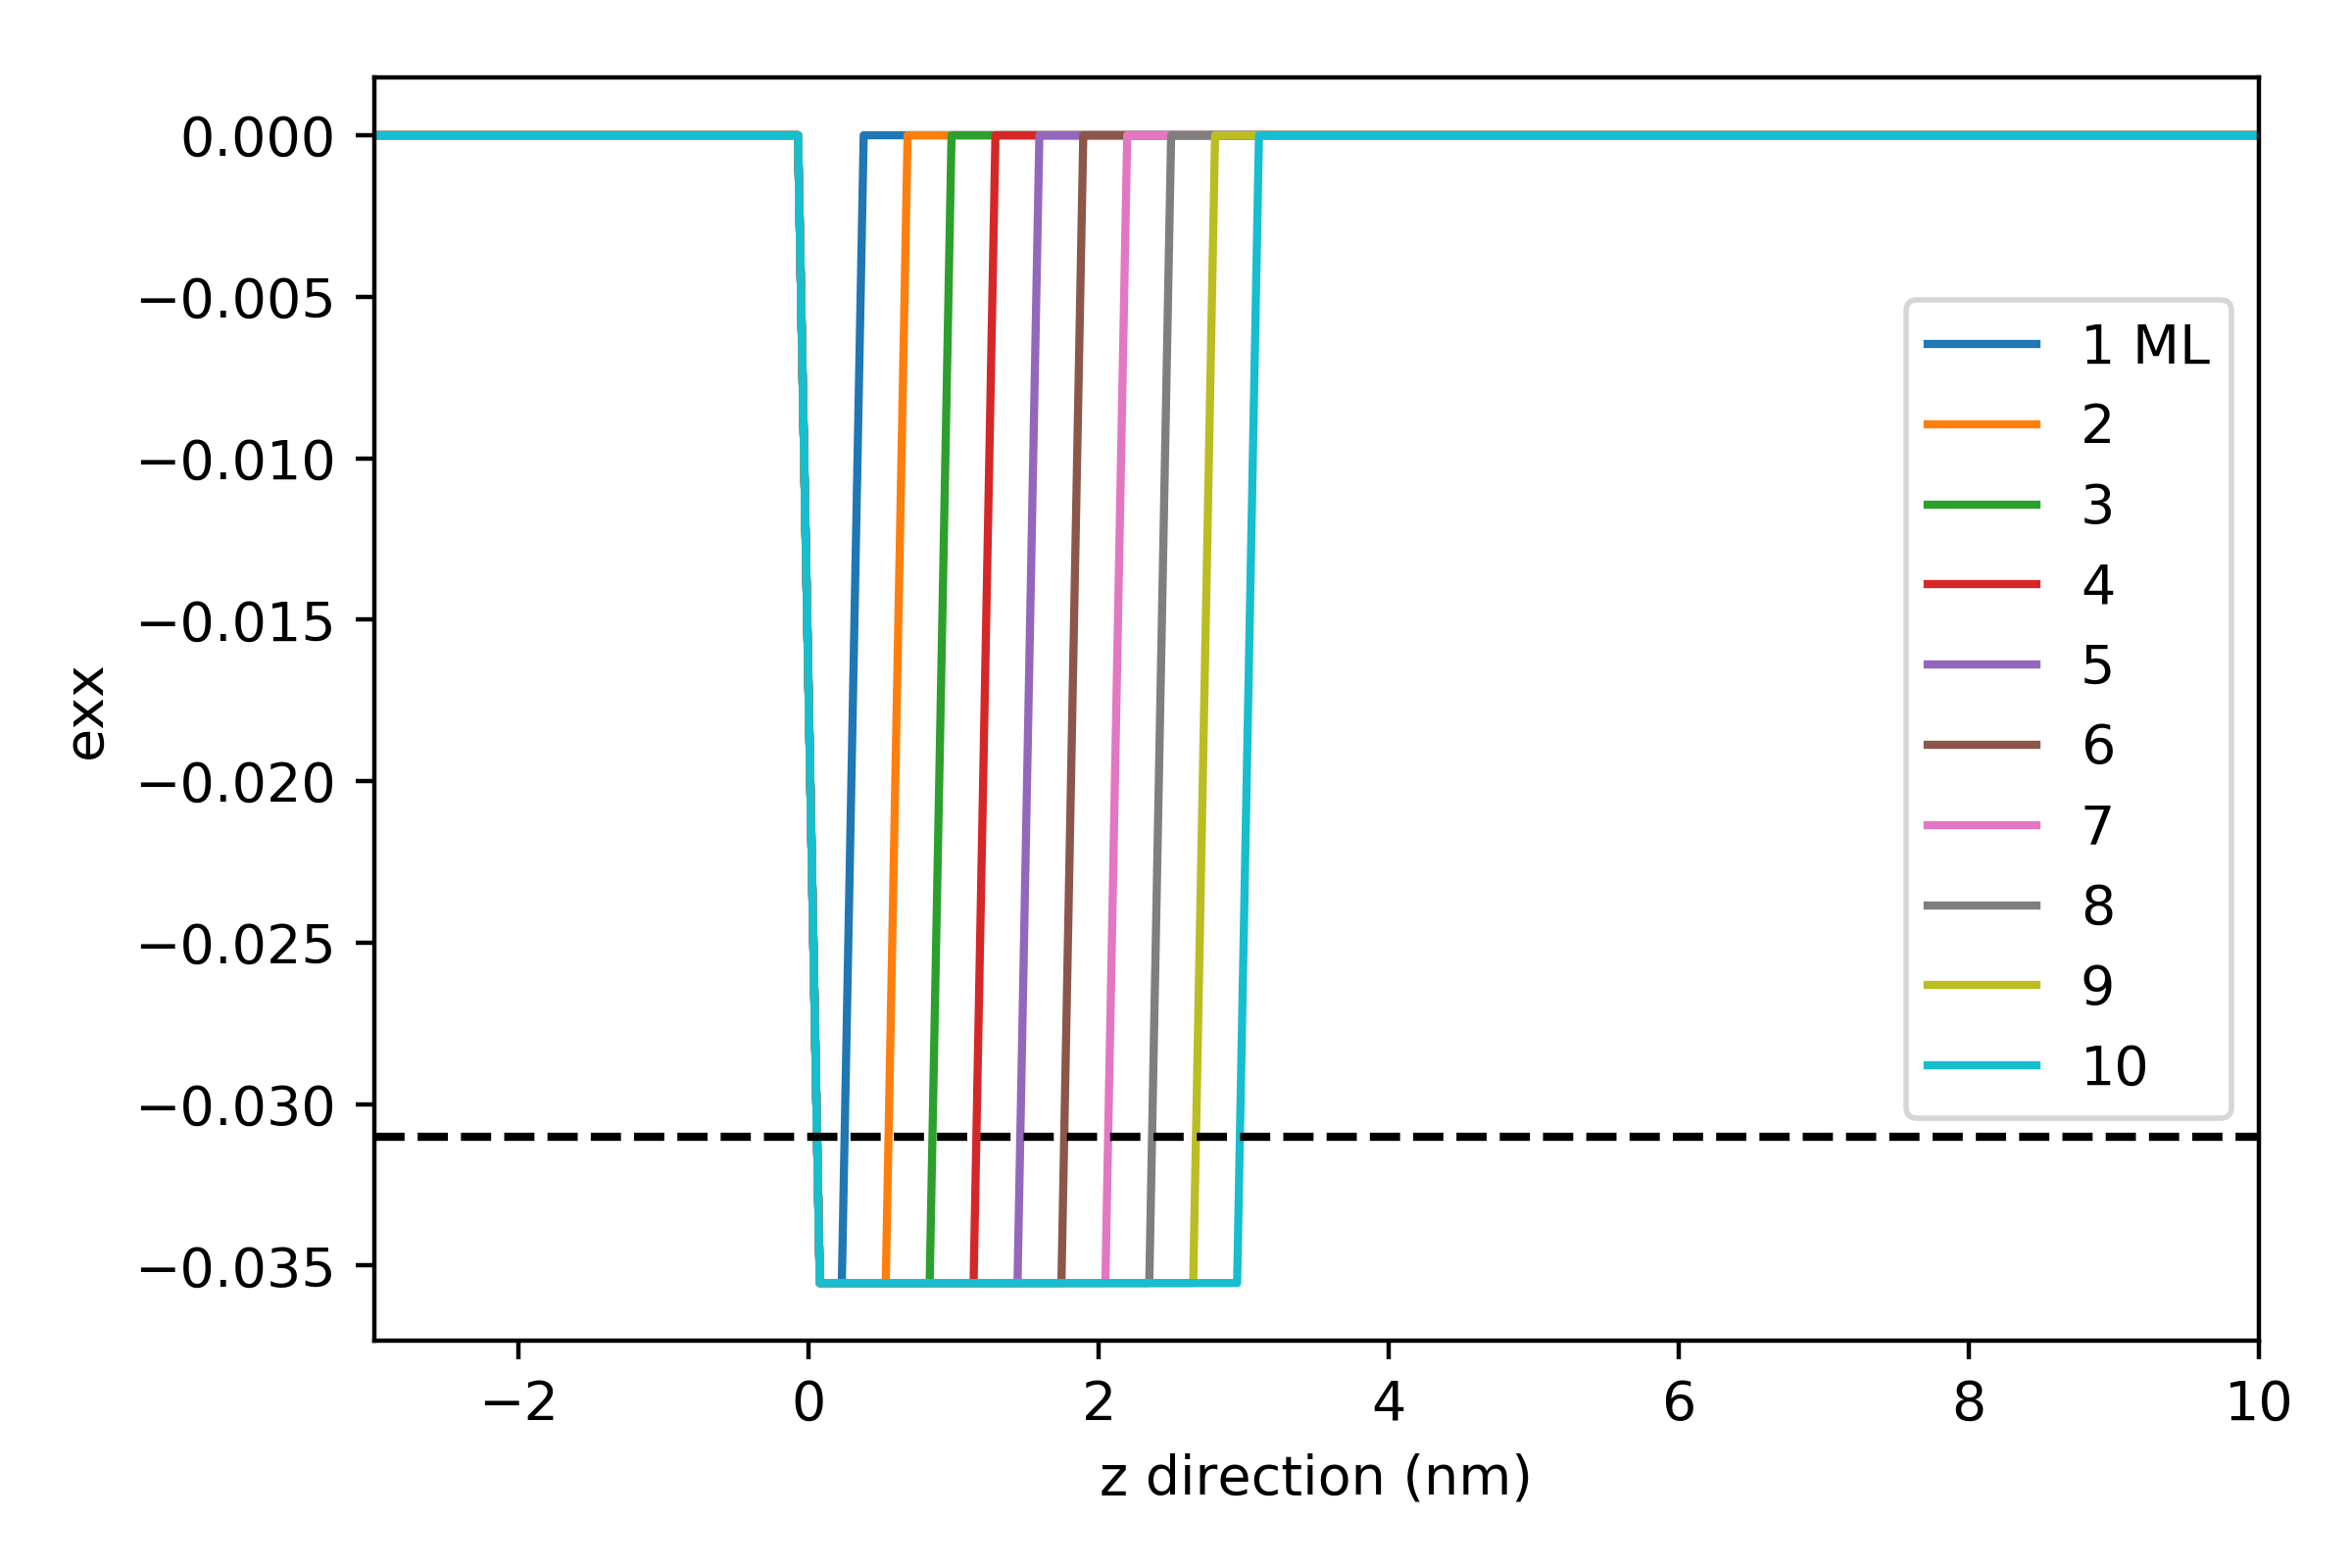
\includegraphics[width=0.85\linewidth]{/raman/eyy_vs_ML}
	\caption{Hydrostatic strain $\epsilon_{xx}$ calculated as a function of GaAs layer thickness in the sample $S_\mathrm{w/o}$. The experimental value is represented by a dashed curve. The calculations were made by the supervisor.}
	\label{fig:raman_theory_wo}
\end{figure}


\clearpage
\section{Experimental setup for photoluminescence measurements}
The PL measurements were performed using standard PL setup. The samples were positioned in the cryostat, cooled to 15~K and pumped by a laser diode with the wavelength of 405~nm with 0.05~mm$^2$ large spot size. The emitted emission signal was dispersed by a 1200~grooves/mm ruled grating designed to the wavelength of 750~nm and synchronously detected by a Si-avalanche photodiode (APD). We have performed the following PL experiments: (i) in intensity dependent measurements the laser power was varied by a neutral density (ND) filter over more than 4 orders of magnitude, (ii) in the temperature resolved PL temperature was changed from 15~K to room temperature, but for our samples and given integration time (0.3~s per one wavelength) we have not detected any PL signal at 300~K, (iii) the polarization of the PL was analyzed by a rotating achromatic half-wave retarder followed by a fixed linear polarizer.

In time-resolved experiments we have used laser with wavelength of 405~nm focused on 0.06~mm$^2$ area with pulse-width of 60~ps; emitted PL spectrum was dispersed again by 1200~grooves/mm ruled grating and detected by a Si-APD. We have performed the following TRPL experiments: (i) intensity resolved TRPL was measured at 15~K in 200~ns temporal window with resolution around 800~ps; the pumping power density was tuned by a ND filter in a range of 0.1--0.7~W/cm$^2$. The repetition rate of the laser was 5~MHz. (ii) In temperature resolved TRPL a temperature was changed on a range 15--150~K, the temporal window was modified to maximize the resolution from 200~ns for lower temperature to 25~ns for higher temperature. Tuning the temporal window is connected with changes in repetition rate, which was varied between 5 (for the temporal window 200~ns) and 80~MHz (for 25~ns).

Both experimental setups are schematically depicted in~\ref{fig:Madrid_setup}.
\begin{figure}
	\centering
	\includegraphics[width=1\linewidth]{/PL/setup}
	\caption{Schematic of the (a) PL and (b) TRPL measurement setup. The picture of the TRPL setup is motivated by Ref.~\citep{TRPL_setup}.}
	\label{fig:Madrid_setup}
\end{figure}


\newpage
\section{Photoluminescence measurements}

The homogeneity of samples was tested by performing PL measurements on different areas of them. The results of those for different samples spots (distinguished by the type of the curve) and samples (different color) are depicted in the Fig.~\ref{fig:PL_homogenity}. We can see that samples are rather spatially homogeneous, hence our measurements might be considered as reproducible on the samples. %it is not necessary measured PL and TRPL in the same time. 

Let look at the emission structures around 1.8~eV. Firstly, we compare substrate emission in this spectral range with signal from our samples. We clearly see a broader band which is around 70~times smaller than emission from our samples so that we neglect this band. For $S_\mathrm{w/o}$ are shown PL with two maxima located at 1.83 and 1.86~eV, respectively. The PL signal of samples with QDs are shifted to smaller energies: the maxima are located at 1.78~eV for $S_\mathrm{with}$ and 1.74~eV for $S_\mathrm{cap}$. Finally, let us notice that the PL from $S_\mathrm{with}$ is twice stronger compared to other samples.
\begin{figure}
	\centering
	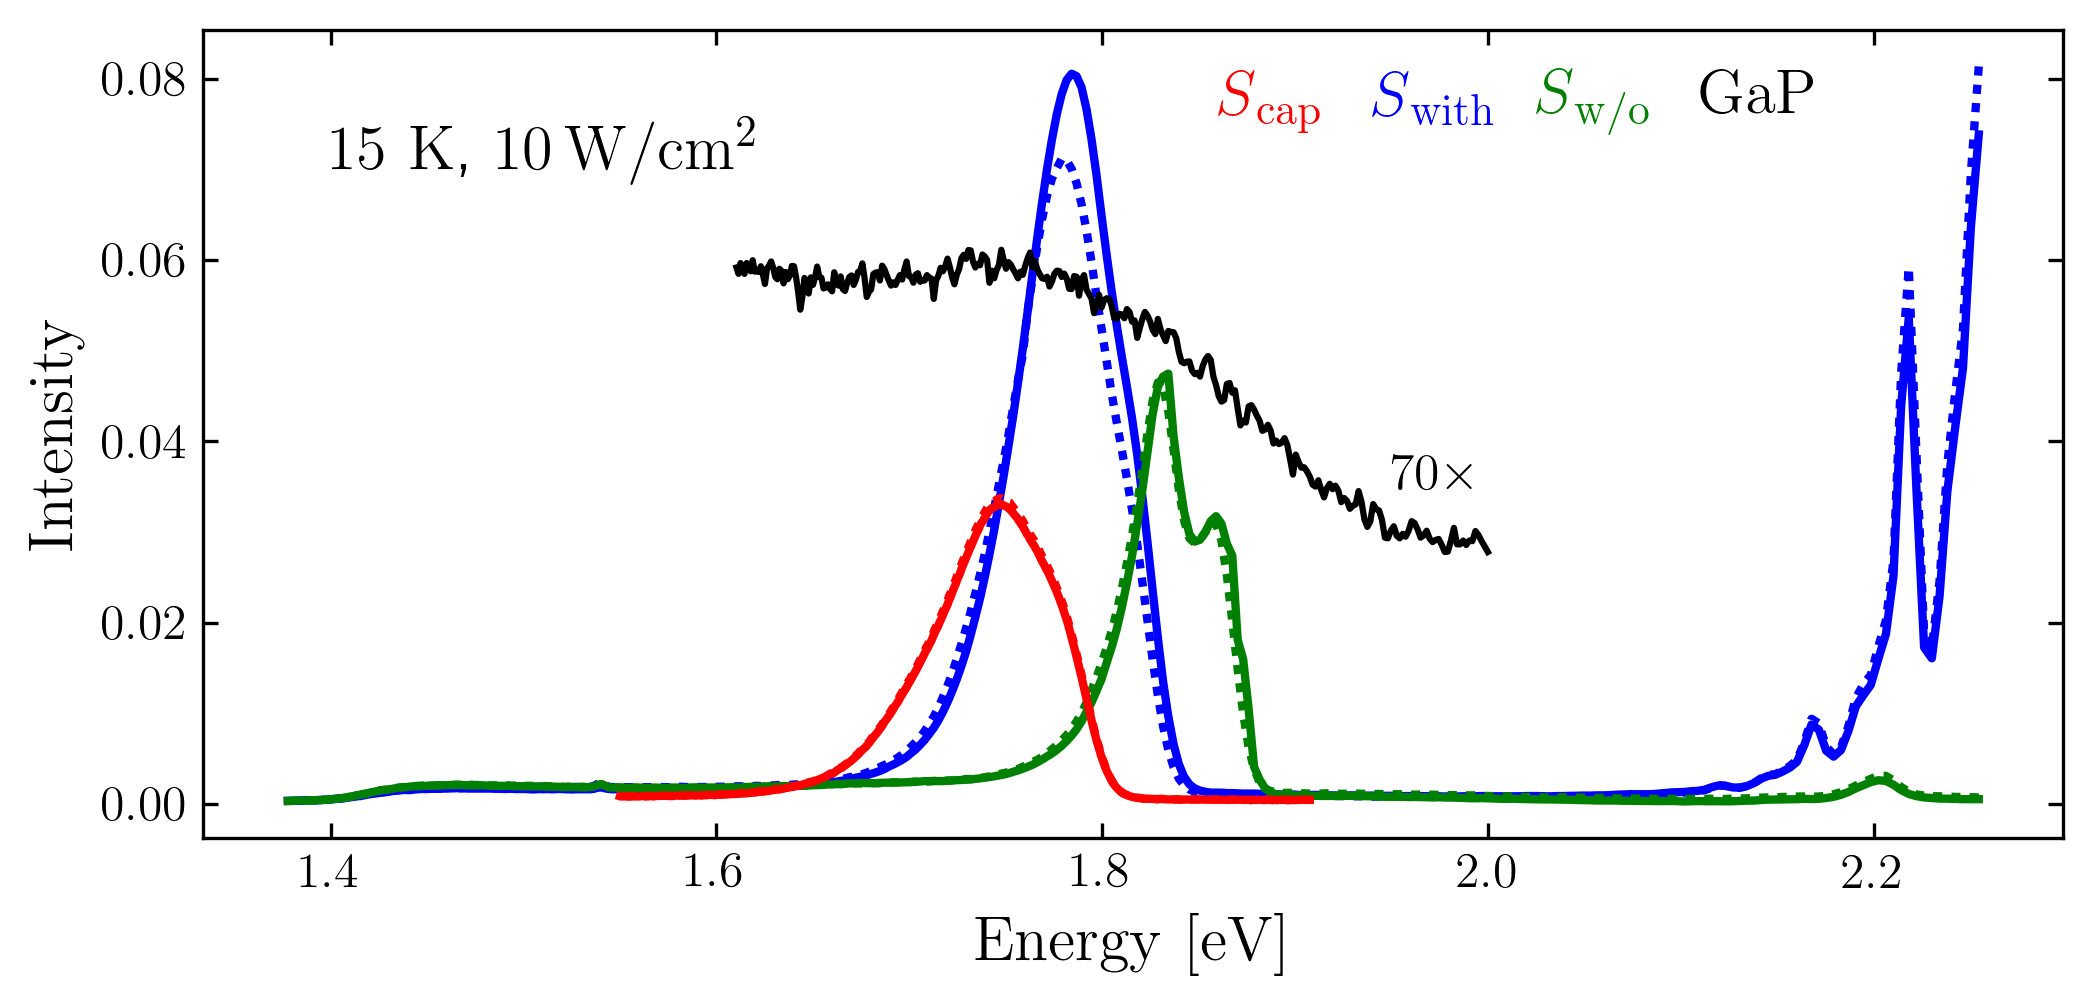
\includegraphics[width=1\linewidth]{/PL/all__IntensityVSen_GaP}
	\caption{PL for samples $S_\mathrm{w/o}$ (green lines), $S_\mathrm{with}$ (blue) and $S_\mathrm{cap}$ (red) measured at 15~K and 10~W/cm$^2$ on several places on samples (different curve types). PL from our samples is compared with emission from GaP substrate (black).}
	\label{fig:PL_homogenity}
\end{figure}

\subsection{Excitation intensity dependent PL}
\label{sec:intensity_PL_TU}
PL for each sample and excitation density $D$ was fitted by sum of three Gaussian curves and the individual bands corresponding to different optical transitions was studied. 

\subsubsection*{Sample without QDs $\mathbf{S_\mathrm{w/o}}$}

\begin{figure}
	\centering
	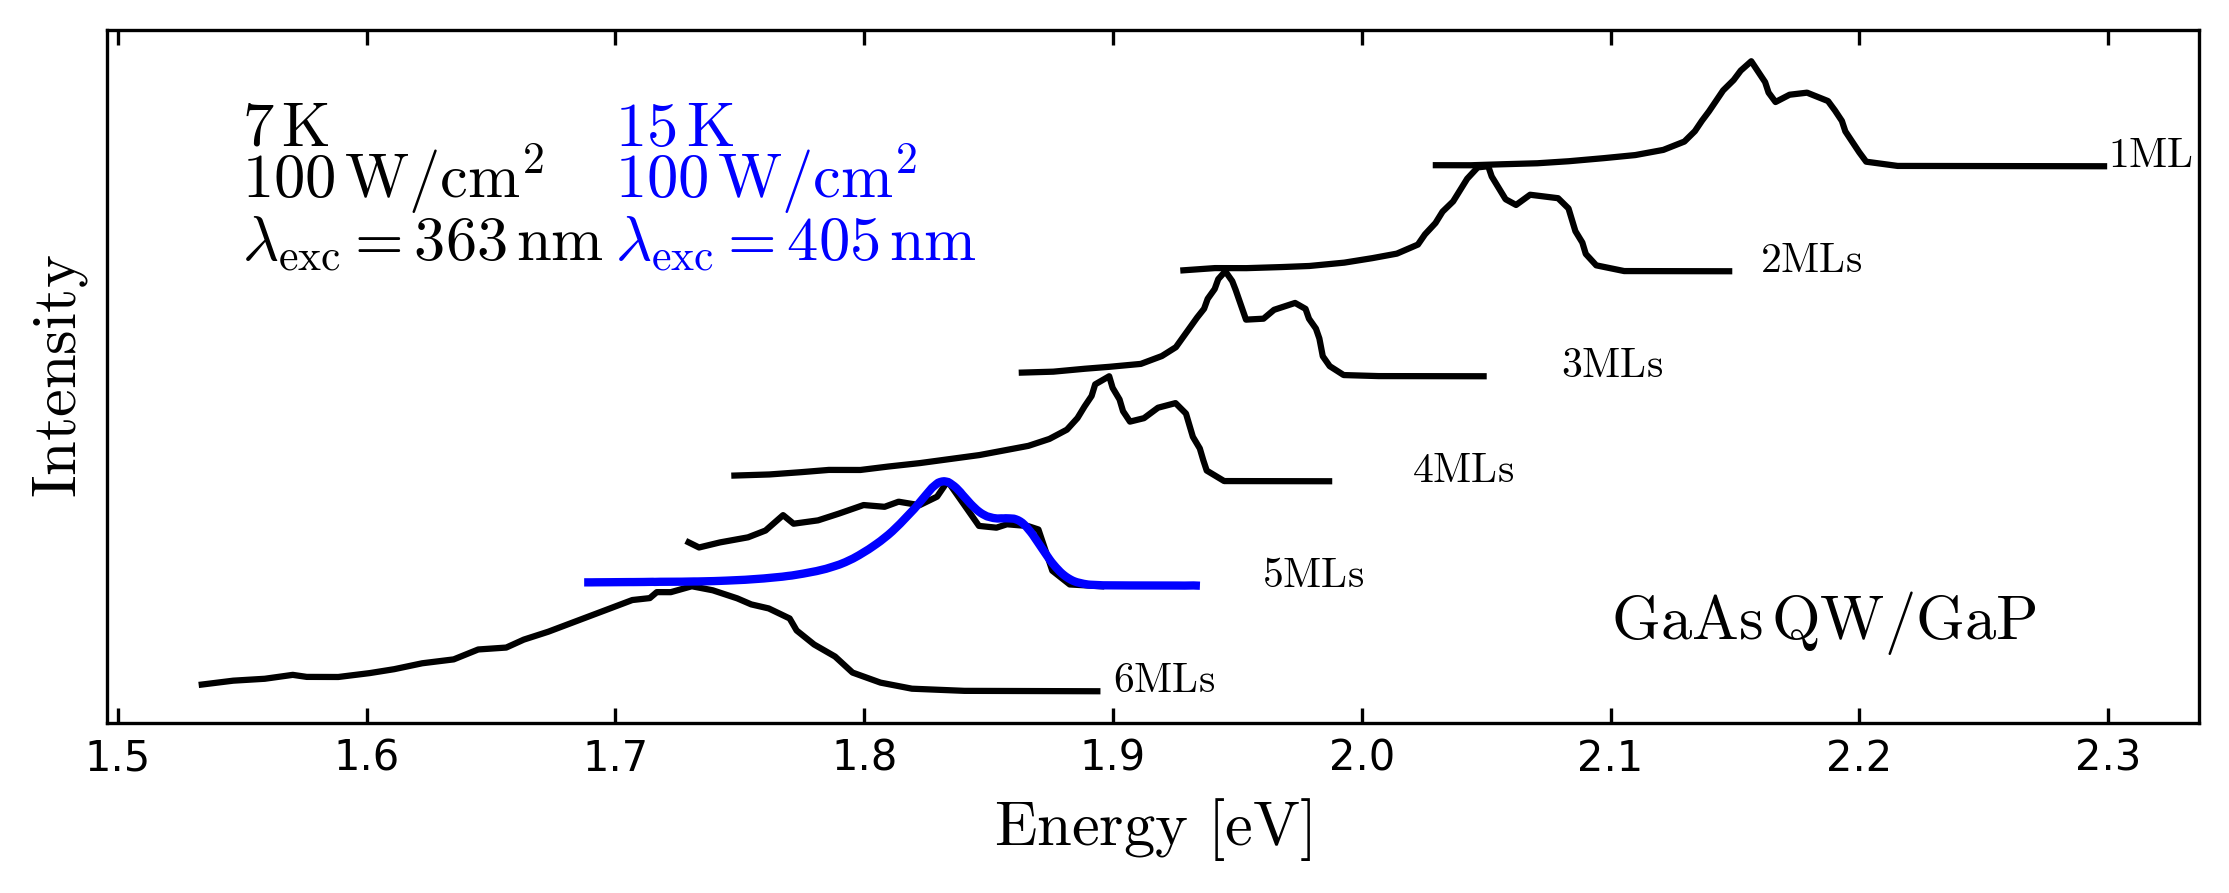
\includegraphics[width=0.9\linewidth]{/PL/12027_ref_GaAs_5ML_new}
	\caption{The comparison of the spectrum of $S_\mathrm{w/o}$ (blue) with set of samples with variable thickness taken from~Ref.~\citep{Prieto_APL1997} (black). The measurement temperature of 15~K (7~K), excitation wavelength of 405~nm (363~nm) in our (in ref.~\citep{Prieto_APL1997}) were used. Excitation density in both experiments was 100~W/cm$^2$. We can see a good match of sample $S_\mathrm{w/o}$ with 5ML thick GaAs QW from Ref.~\citep{Prieto_APL1997}.}
	\label{fig:12027_ref}
\end{figure}


\begin{figure}
	\centering
	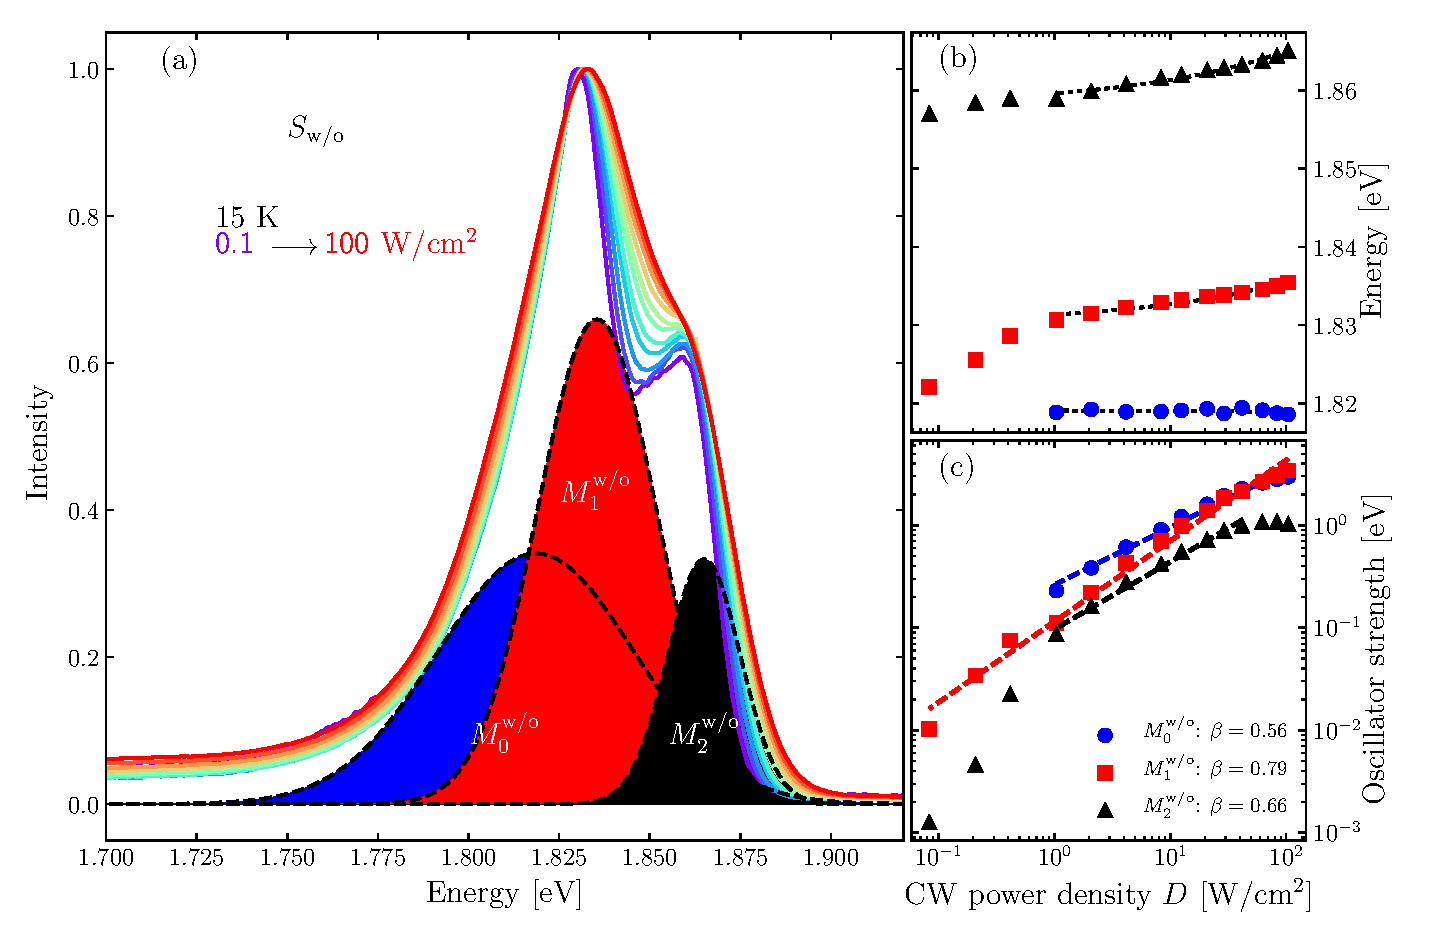
\includegraphics[width=0.9\linewidth]{/PL/intensity/12027_11011_norm_PL_int}
	\caption{(a) PL spectra of $S_\mathrm{w/o}$ measured for several excitation density in the range 0.1 and 100~W/cm$^2$. The fit by the sum of three Gaussian curves is shown for 100~W/cm$^2$ and the individual bands are presented by shaded area: $M_0^\mathrm{w/o}$ (blue), $M_1^\mathrm{w/o}$ (red) and $M_2^\mathrm{w/o}$ (black). In (b) we show power dependence of the energy of individual bands and their fits by Eq.~\ref{eq:PL_intmodel} (dotted curves). Panel (c) depicts the oscillators strength of the bands in log-log scale and their fits by linear lines (broken lines), respectively. The slopes of the linear fit $\beta$ (exponent in linear scale) are presented in the legend of panel (c). Individual transitions in panels (b) and (c) are represented by: $M_0^\mathrm{w/o}$ (blue circles), $M_1^\mathrm{w/o}$ (red squares) and $M_2^\mathrm{w/o}$ (black triangles).}
	\label{fig:QD_wo_int}
\end{figure}
Three emission bands of sample $S_\mathrm{w/o}$ labelled from smaller to greater localization energy $M_0^\mathrm{w/o}$, $M_1^\mathrm{w/o}$ and $M_2^\mathrm{w/o}$, respectively, are related to electrons in the $X_{xy}$ (the $X$ bands for GaAs strained to GaP are split into $X_z$ and $X_{xy}$ where $z$ indicates growth direction) GaAs minima recombination with heavy holes in the $\Gamma$ band in GaAs layer. Ref.~\citep{Prieto_APL1997} discusses the effect of GaAs layer thickness on emission spectra where they observed overally an energy shift, with the thickness of the layer, but the energy separations between corresponding bands stayed nearly independent of layer thickness. Similarly as in Ref.~\citep{Prieto_APL1997}, where those were 12 and 32~meV, we detect similar ones and depending on the excitation density we have found them to be between 12--17~meV and 40--46~meV. Hence, the peaks cannot be attributed to thickness fluctuations, but instead they can be connected with phonon-assisted transitions. The energies of the phonons closely correspond to TA and LA phonon energies in GaP~\citep{Prieto_APL1997}. In Fig.~\ref{fig:12027_ref} PL of $S_\mathrm{w/o}$ is compared with studied set taken from Ref.~\citep{Prieto_APL1997}.



In Fig.~\ref{fig:QD_wo_int}(a) we show PL spectra of the sample with increasing $D$ and their deconvolution into individual band by Gaussian fits. The energy-shift is visualized in Fig.~\ref{fig:QD_wo_int}(b), where PL peak energies as a function $D$ for individual bands are plotted and fitted with usually used formula~\citep{Hatami_apl1995_intmodel,Glaser_apl1996_intmodel,Ledentsov_prb1995_intmodel} derived for spatially indirect optical transition in quantum wells (QWs) and QDs
%
\begin{equation}
E(D)=E_\mathrm{I}+\gamma D^{1/3}, \label{eq:PL_intmodel}
\end{equation}
%
where $E_\mathrm{I}$ is extrapolation energy to $D=0$~W/cm$^2$ and $\gamma$ is proportional constant which describes the gradient of the energy-shift. The energy evolutions of the bands are well characterized with~Eq.~(\ref{eq:PL_intmodel}). The bands $M_1^\mathrm{w/o}$ and $M_2^\mathrm{w/o}$ are slightly shifted to blue with increasing $D$, these blue-shifts are described by almost identical $\gamma$, whereas $M_0^\mathrm{w/o}$ is rather independent on $D$ or slightly red-shifted.






The oscillator strengths in Fig.~\ref{fig:QD_wo_int}(c) of $M_0^\mathrm{w/o}$, $M_1^\mathrm{w/o}$ follow a linear dependence in log-log graph with the excitation power in the whole measured range, indicating that there is neither saturation of electronic states nor the activation of the non-radiative events. The emission of $M_2^\mathrm{w/o}$ is linear only in the power density range 1 and 30~W/cm$^2$, under the range PL is saturated.

%%%%%%%%%%%%%%%%%%%%%%%%%%%%%%%%%%%%%%%%%%%%%%%
\subsubsection*{Sample with QDs $\mathbf{S_\mathrm{with}}$}
\begin{figure}
	\centering
	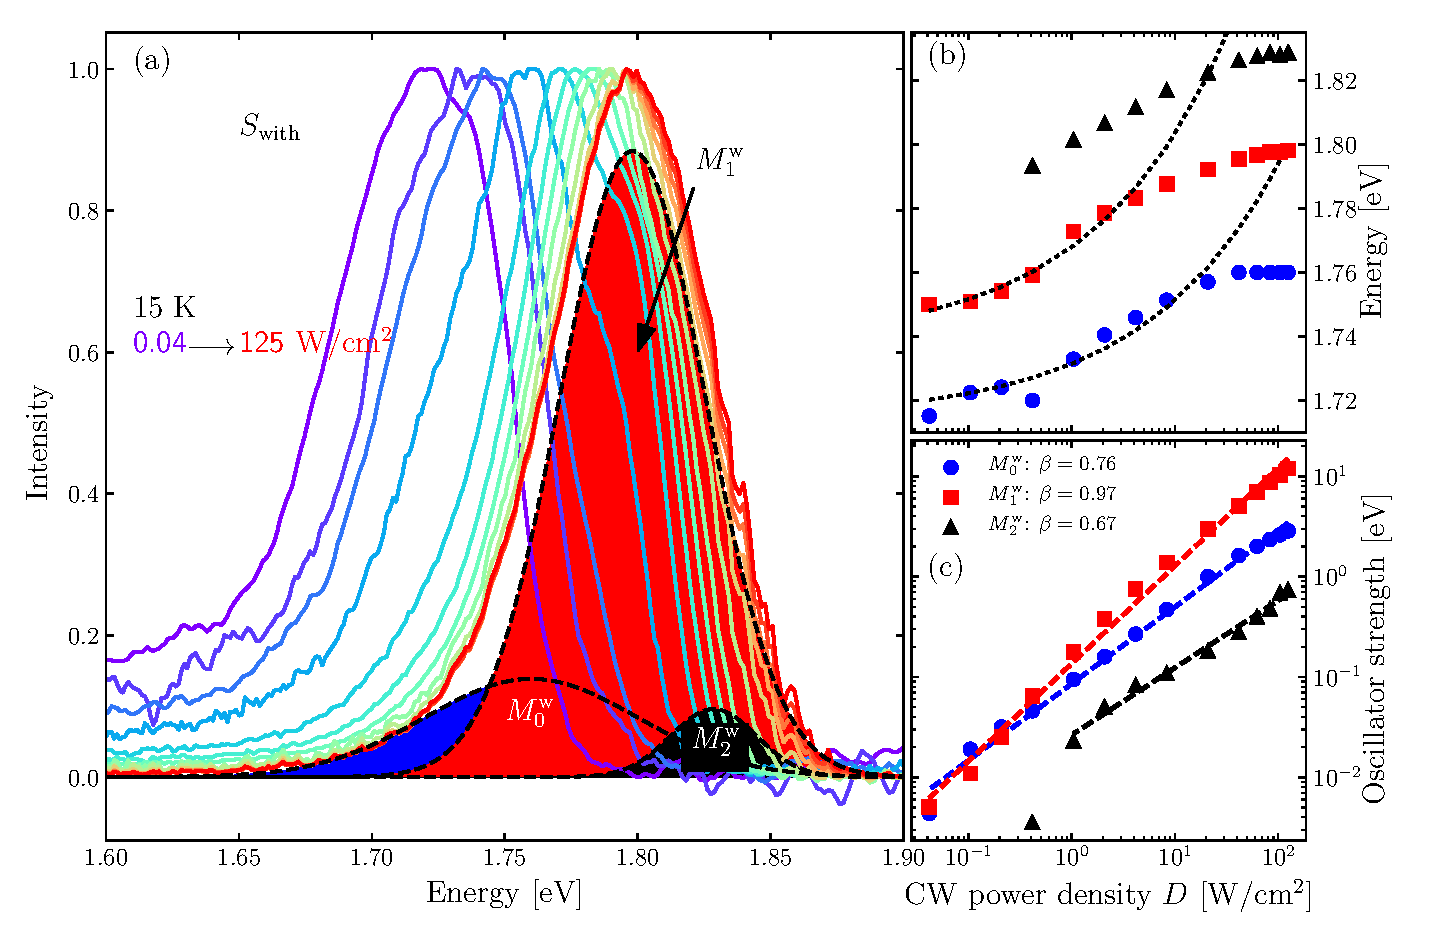
\includegraphics[width=0.9\linewidth]{/PL/intensity/12040_1113_norm_PL_int}
	\caption{(a) PL spectra of $S_\mathrm{with}$ as a function of excitation density were measured from 0.04 to 125~W/cm$^2$ and deconvolved by three Gaussian profiles ($M_0^\mathrm{w}$ blue, $M_1^\mathrm{w}$ red and $M_2^\mathrm{w}$ black shaded area). Fitted parameters - energy and oscillator strength are depicted in panels (b) and (c), respectively. Energies are fitted by Eg.~\ref{eq:PL_intmodel} (dotted curves in (b)), oscillator strengths by linear curve (dashed lines in (c)).}
	\label{fig:QD_w_int}
\end{figure}

Three Gaussian profiles ($M_0^\mathrm{w}$, $M_1^\mathrm{w}$ and $M_2^\mathrm{w}$) in PL spectra were fitted and studied as a function of excitation density $D$ in the range between 0.04 and 125~W/cm$^2$, see Fig.~\ref{fig:QD_w_int}. In Fig.~\ref{fig:QD_w_int}(b) and (c) we show the emission energy and oscillator strength of individual bands as a function of $D$, respectively. The energies of $M_0^\mathrm{w}$ and $M_1^\mathrm{w}$ are fitted by Eq.~\ref{eq:PL_intmodel}, but we can see the third root behaviour only in the beginning of the dependence, then the energies start to be saturated. The whole evolution of energy versus pumping power is much better characterized using the self-consistent multi-particle calculations as in Ref.~\citep{Klenovsky2017}.

The dependencies for oscillator strengths were fairly well fitted by the linear function in the whole range.




\subsubsection*{Sample with capped QDs $\mathbf{S_\mathrm{cap}}$}
\begin{figure}
	\centering
	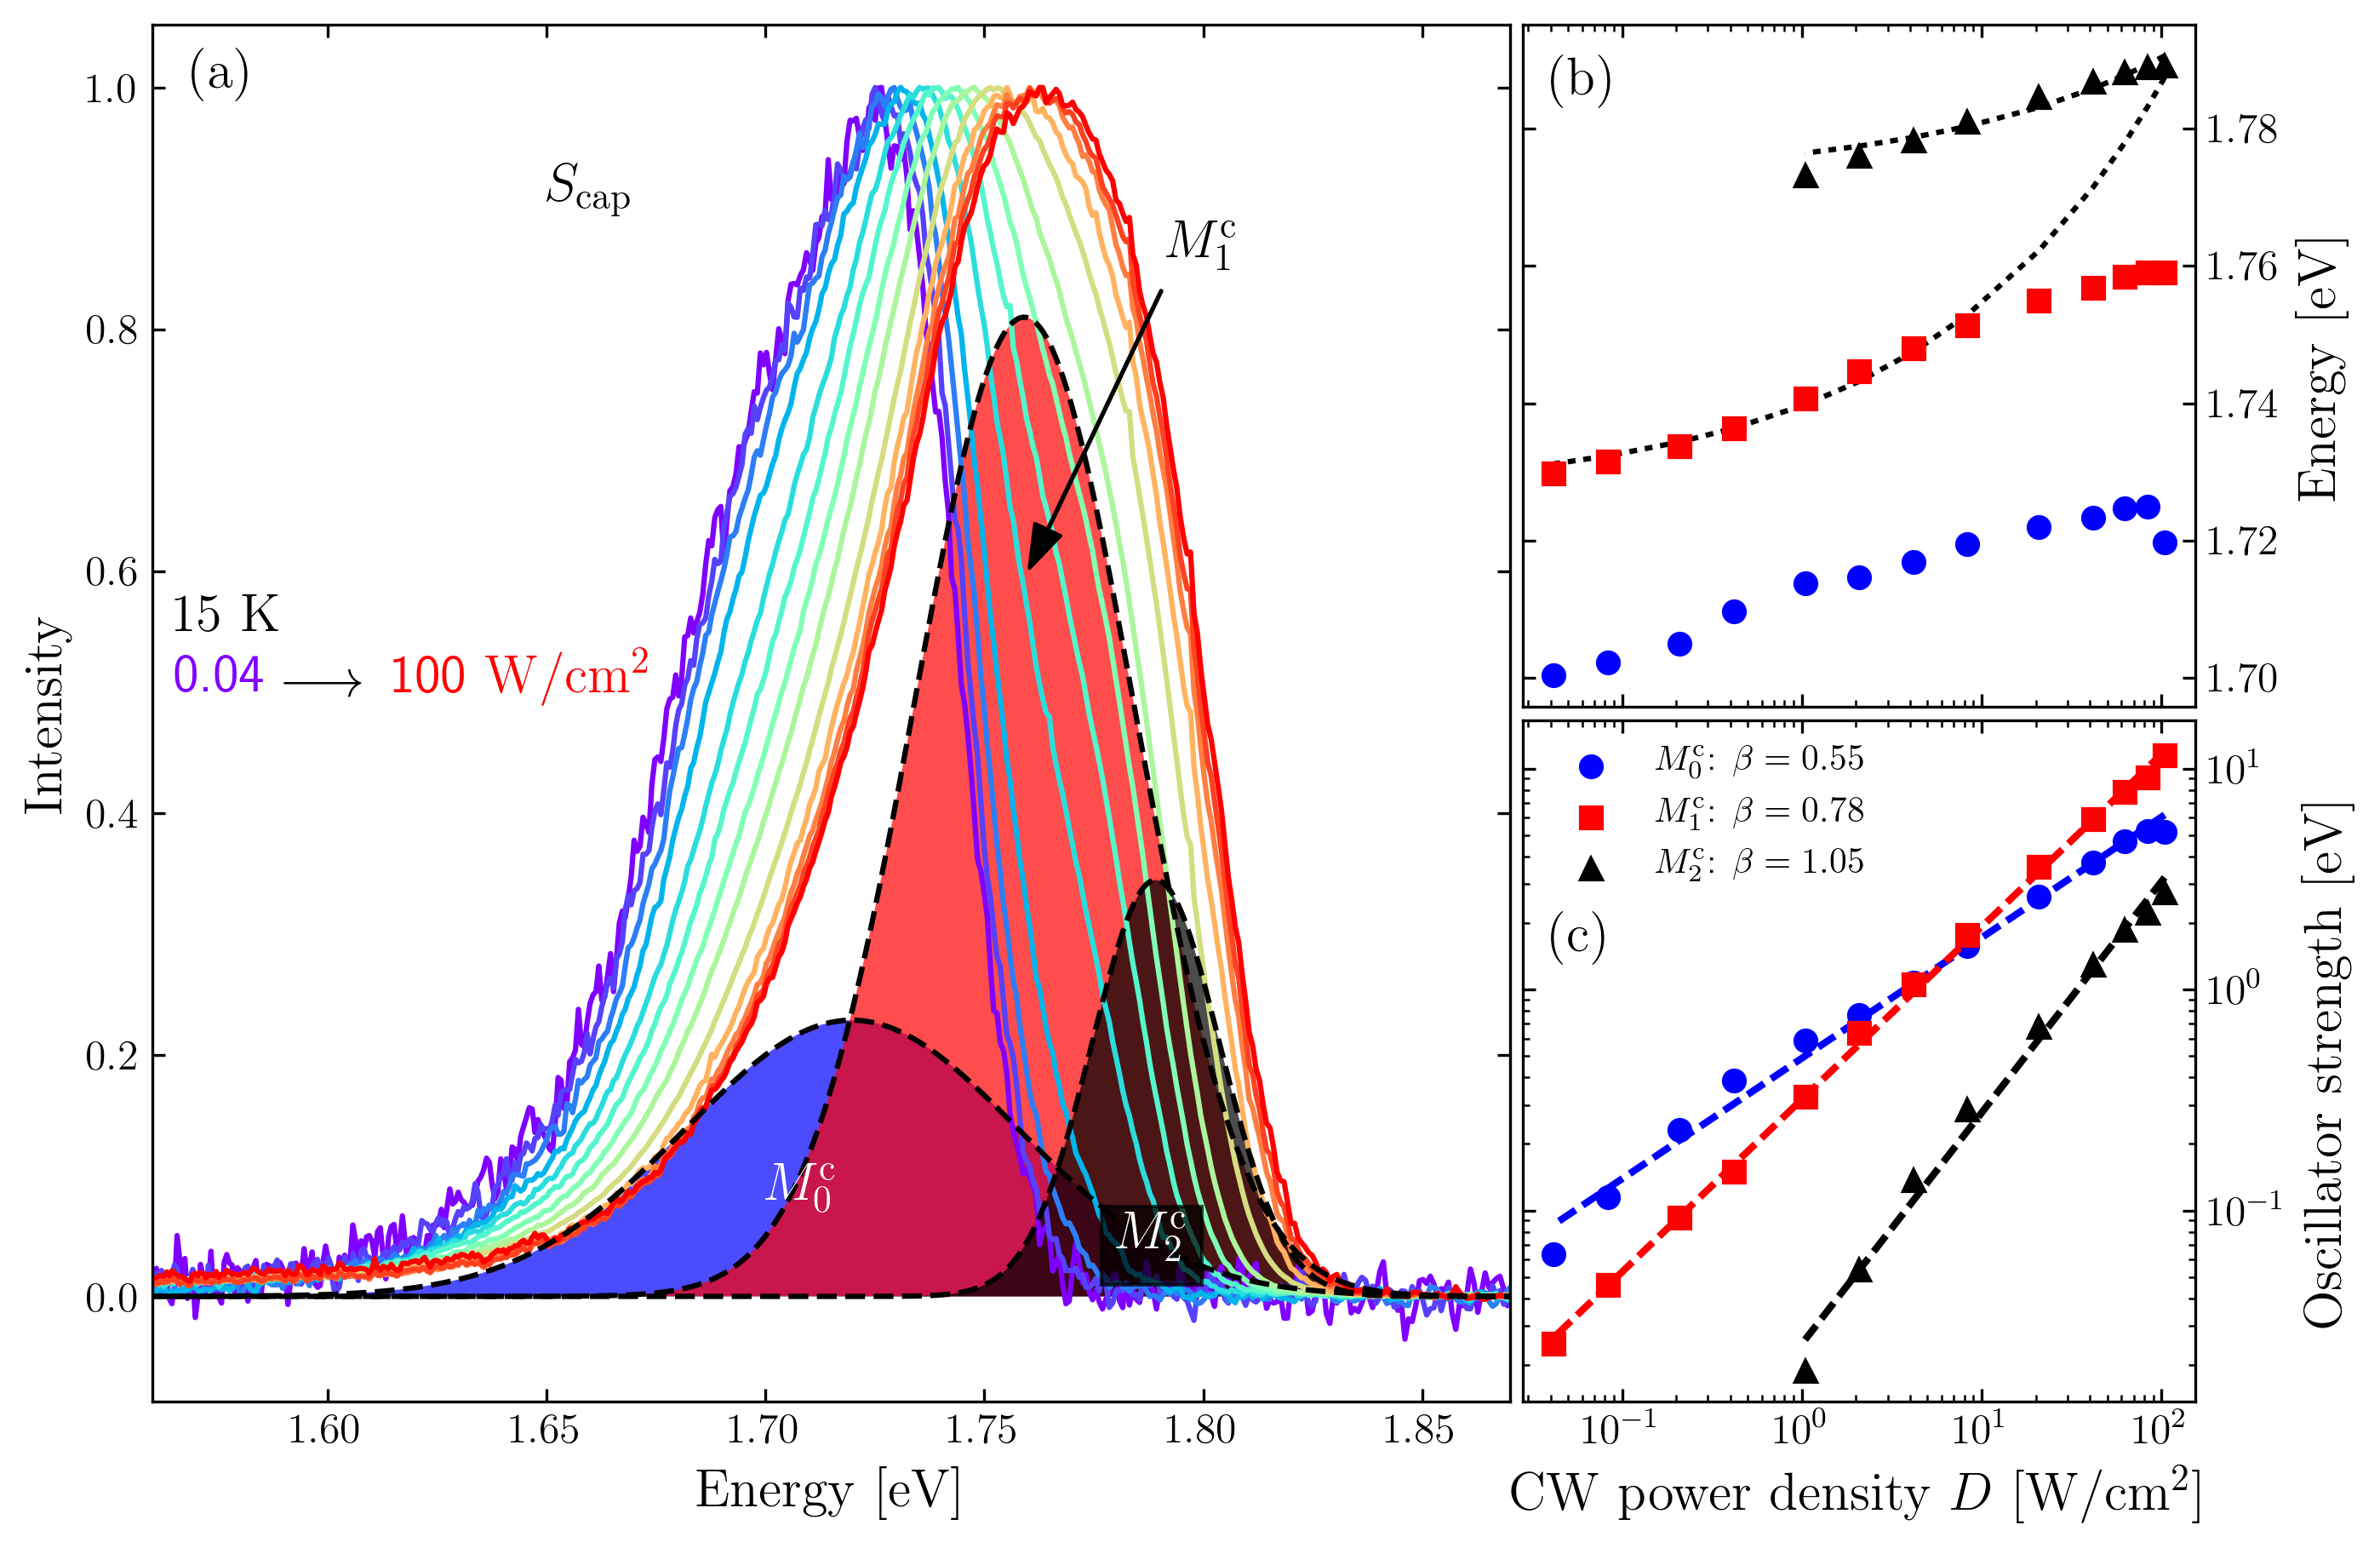
\includegraphics[width=0.9\linewidth]{/PL/intensity/12021_1108_norm_PL_int}
	\caption{The results are given in the same nomenclature as in Fig.~\ref{fig:QD_w_int}.}
	\label{fig:QD_cap_int}
\end{figure}

Intensity-resolved PL spectra of ${S_\mathrm{cap}}$ were treated similarly as for sample ${S_\mathrm{with}}$ and can be seen in Fig.~\ref{fig:QD_cap_int}. All fitted parameters are summarized in Tab.~\ref{tab:int_params}.
\begin{table}
	\centering
	\caption{Summary of the fitting parameters of power density dependent PL for all samples.}
	\begin{tabularx}{0.75\textwidth}{cCCc}
		\toprule
		
		transition & $E_\mathrm{I}$ [meV]& $\gamma$ [$10^{-5}$]& $\beta$ [$\mathrm{W^{2/3}cm^{2/3}s^{-2/3}}$]\\ 	
		\midrule
		\midrule
		$M_0^\mathrm{w/o}$& $1819\pm1$ & $-5\pm6$& $0.55\pm0.02$\\
		$M_1^\mathrm{w/o}$& $1830\pm1$ & $114\pm9$& $0.79\pm0.02$\\
		$M_2^\mathrm{w/o}$ & $1858\pm1$ & $148\pm9$& $0.66\pm0.03$\\ 
		
		\midrule
		$M_0^\mathrm{w}$& $1714\pm3$ & $1700\pm200$& $0.76\pm0.06$\\
		$M_1^\mathrm{w}$& $1737\pm3$ & $3100\pm300$& $0.97\pm0.02$\\
		$M_2^\mathrm{w}$ & -& -& $0.67\pm0.03$\\ 
		
		\midrule
		$M_0^\mathrm{c}$& - & -& $0.54\pm0.02$\\
		$M_1^\mathrm{c}$& $1727\pm1$ & $1290\pm80$& $0.78\pm0.01$\\
		$M_2^\mathrm{c}$ & $1772\pm1$ & $380\pm30$& $1.05\pm0.04$\\
		
		\bottomrule
	\end{tabularx}\label{tab:int_params}
\end{table}

The evolution of the emission bands of sample $S_\mathrm{cap}$ with excitation intensity is compared with predictions obtained within the semi-self-consistent CI (SSCCI) presented in Ref.~\citep{Klenovsky2017} %and described in chapter~\ref{chap:SciRep} 
for 2.5~nm height In$_{0.15}$Ga$_{0.85}$As$_{0.85}$Sb$_{0.15}$/GaAs/GaP QD by the supervisor. The band $M_1^\mathrm{c}$ is reasonably well reproduced by SSCCI with basis formed from single-particle wavefunctions calculated by $1\times8~\mathbf{k \cdot p}$ method with electrons originating from $L$ and holes form $\Gamma$-point. On the other hand, SSCCI with $8\times8~\mathbf{k \cdot p}$ basis for electrons coming from $\Gamma$-point can desbribe the band $M_2^\mathrm{c}$.
\begin{figure}
	\centering
	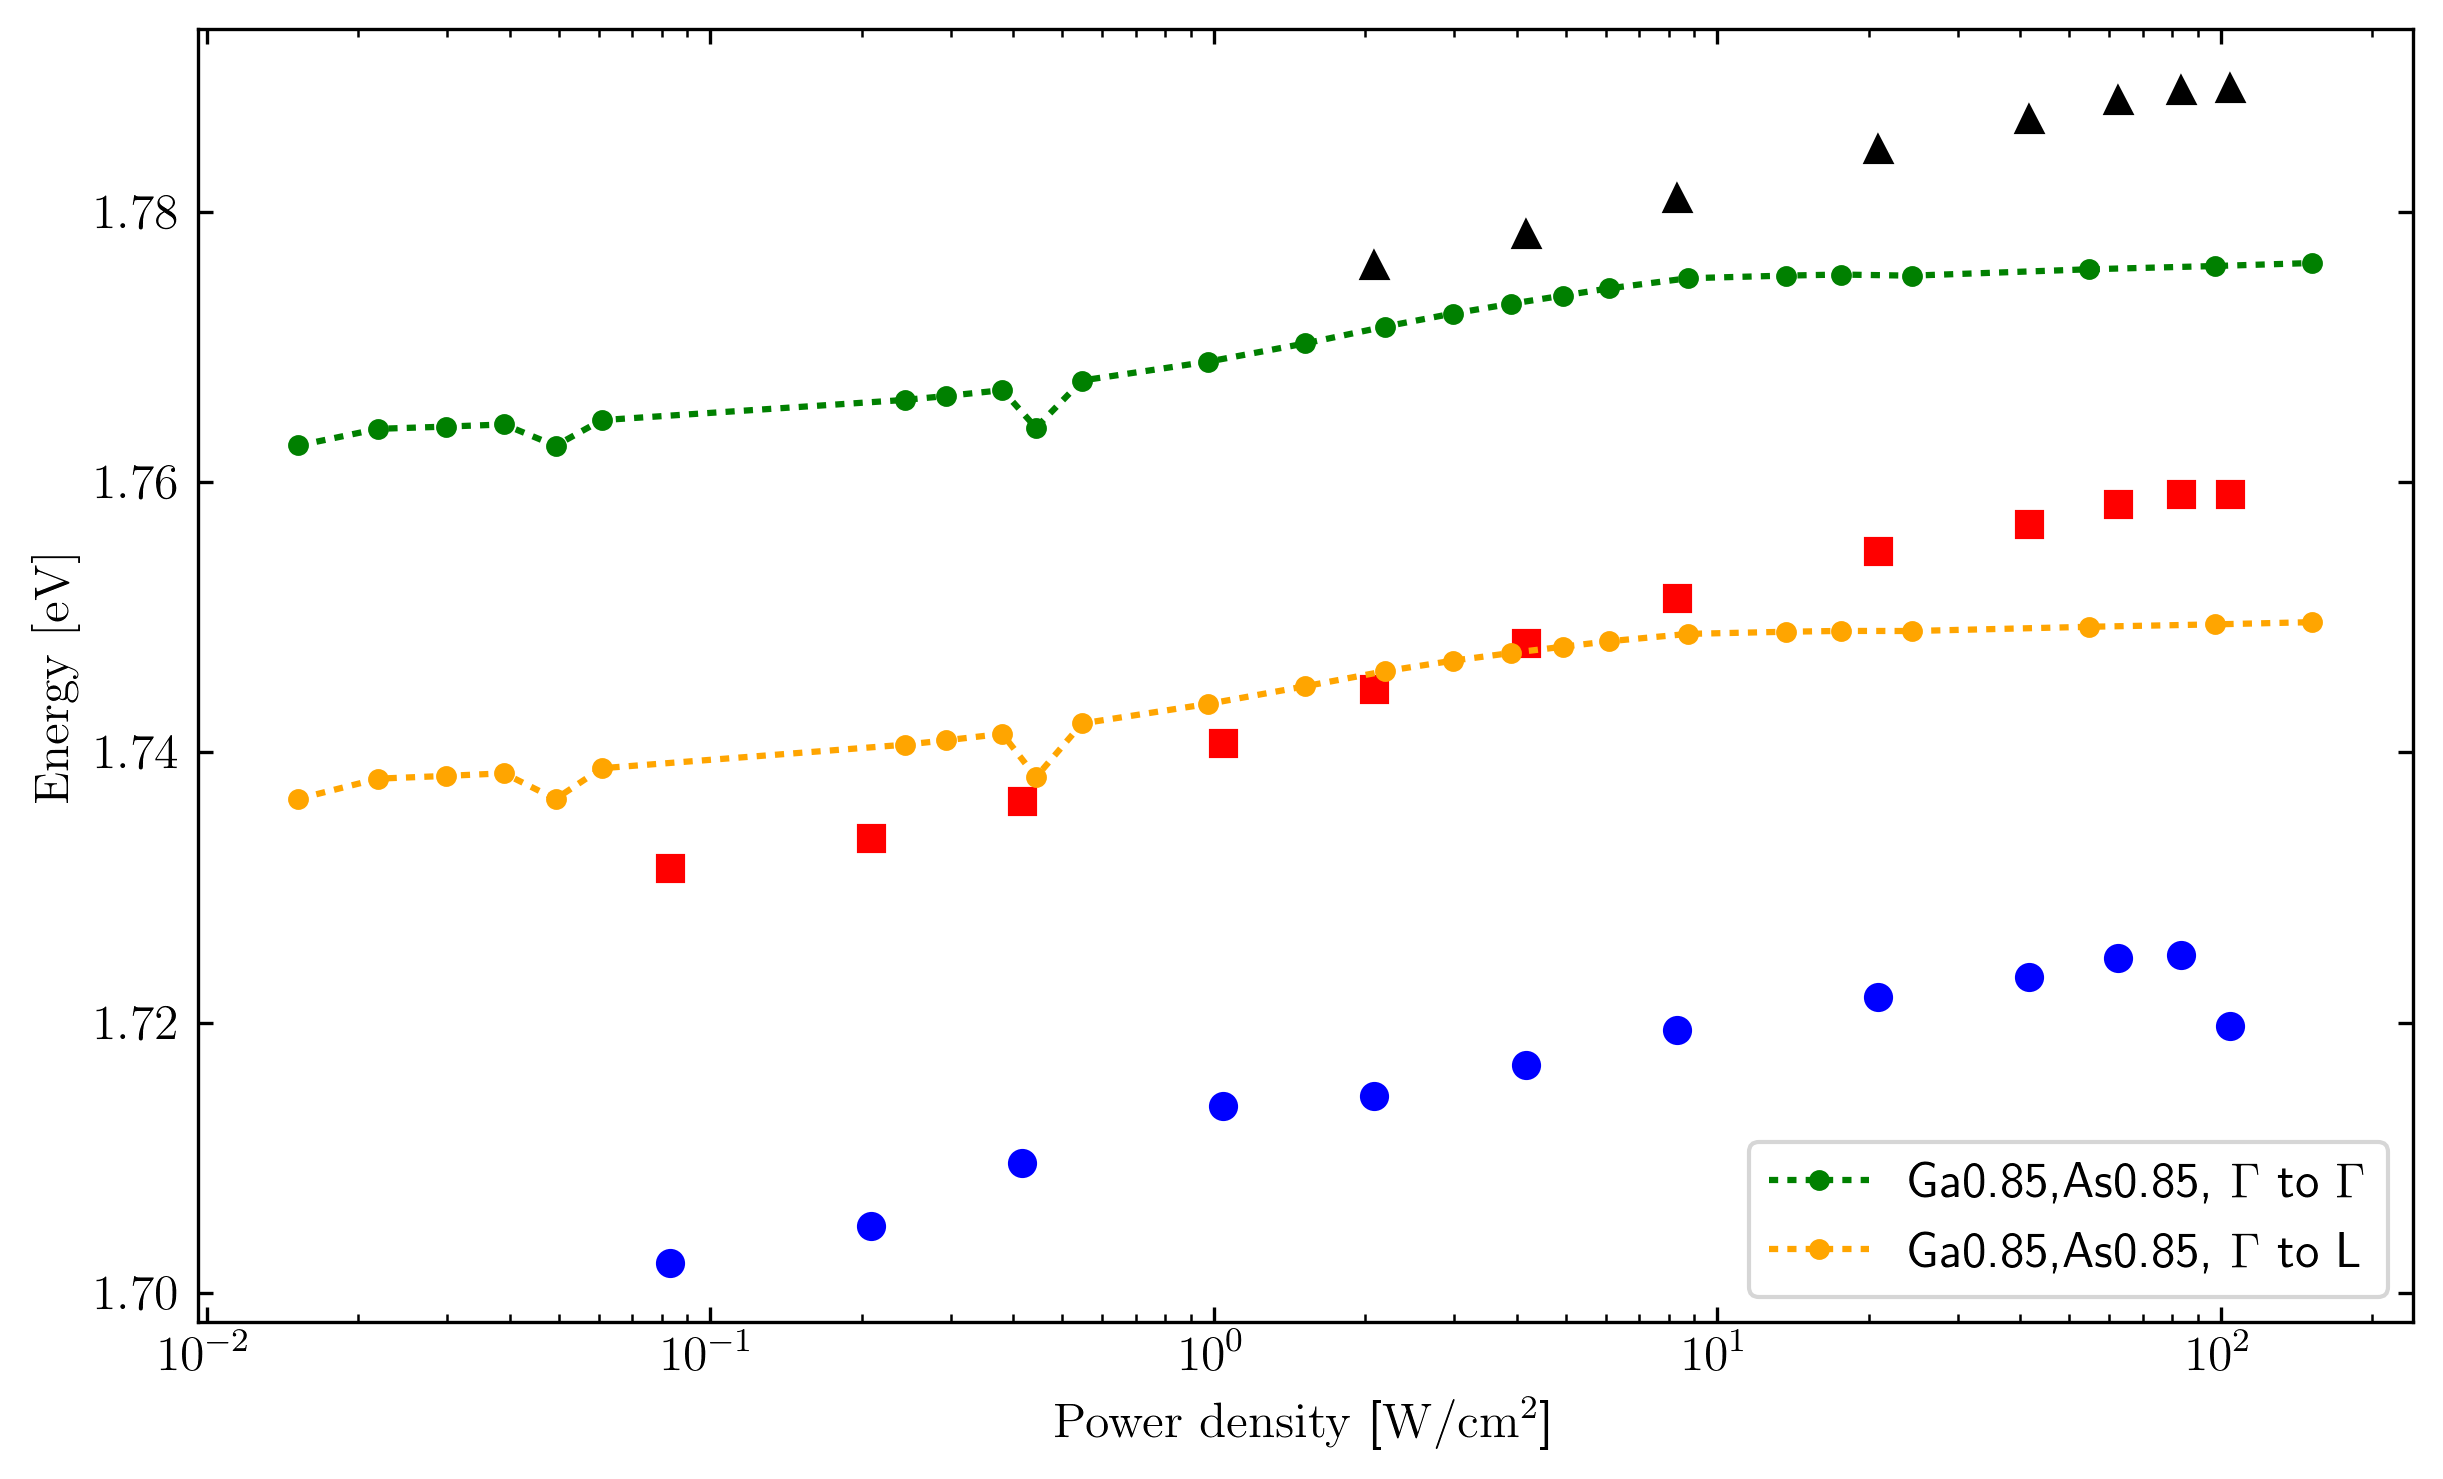
\includegraphics[width=0.9\linewidth]{/PL/intensity/S_cap_expvskpcalc}
	\caption{Emission energy evolution with excitation intensity predicted by SSCCI with single-particle bases calculated by $1\times8~\mathbf{k \cdot p}$ and $8\times8~\mathbf{k \cdot p}$, respectively (dotted curve). To compare experimental points are added.}
	\label{fig:QD_cap_int_expvstheory}
\end{figure}

\newpage
\subsection{Temperature dependent PL}
\label{Sec:temp_PL_TU}
The temperature dependences of the PL of the studied samples was fitted by three Gaussian profiles as in the excitation density investigation in Sec.~\ref{sec:intensity_PL_TU}. The fitted energies were examined using the Varshni-like model
%
\begin{equation}
E(T)=E_0-\frac{\alpha T^2}{T+\Theta_\mathrm{D}}-\frac{\sigma^2}{k_\mathrm{B}T}, \label{eq:Varshni-like}
\end{equation}
where $E_0$ is the energy at temperature $T=0~\mathrm{K}$, $\alpha$ and $\Theta_\mathrm{D}$ are the Varshni parameters, $k_\mathrm{B}$ is Boltzmann constant. The model provides the thermally dependent correction of the empirical Varshni model~\citep{Varshni} describing temperature effects to a band gap of an idealized bulk semiconductor. The estimation proposed by Eliseev~\citep{Eliseev_apl2003_PLtemp} to evaluate the correction is used, which assumes the Gaussian-type distribution of energy of the localized states with broadening parameter $\sigma$.

The mechanisms responsible for the temperature quenching of PL intensity can be accounted for by a Boltzmann model for excitonic recombination with two characteristic activation energies~\citep{Daly_prb1995, Alen_apl2011}
\begin{equation}
I_\mathrm{PL}(T)=\frac{I_0}{1+\tau_0\left[\Gamma_1\exp(-E_1/k_\mathrm{B}T)+\Gamma_2\exp(-E_2/k_\mathrm{B}T)\right]},               \label{eq:Arhenius}
\end{equation}
where $I_0$ is the intensity at 0~K, $\tau_0$ temperature-independent radiative recombination time at 15~K, $E_1$ and $E_2$ are the activation energies of the two quenching mechanisms with related scattering rates $\Gamma_1$ and $\Gamma_2$.%These parameters are representative of the average behaviour of the emissions bands, being the most important $\tau_0$, $E_1$ and $E_2$.
\newpage
\subsubsection*{Sample without QDs $\mathbf{S_\mathrm{w/o}}$}
%
Three recognized emission bands ($M_0^\mathrm{w/o}$, $M_1^\mathrm{w/o}$ and $M_2^\mathrm{w/o}$) in PL of ${S_\mathrm{w/o}}$ are individually investigated from 15~K to 220~K. In this range we can observe Varshni energy-shift of $M_1^\mathrm{w/o}$ and $M_2^\mathrm{w/o}$ described by parameters listed in Tab.~\ref{tab:Varshni}, see Fig.~\ref{fig:QD_wo_temp}(b). In Fig.~\ref{fig:QD_wo_temp}(c) intensity quenching through the temperature range evaluated by the Boltzmann model~(\ref{eq:Arhenius}) is depicted.
%
\begin{figure}
	\centering
	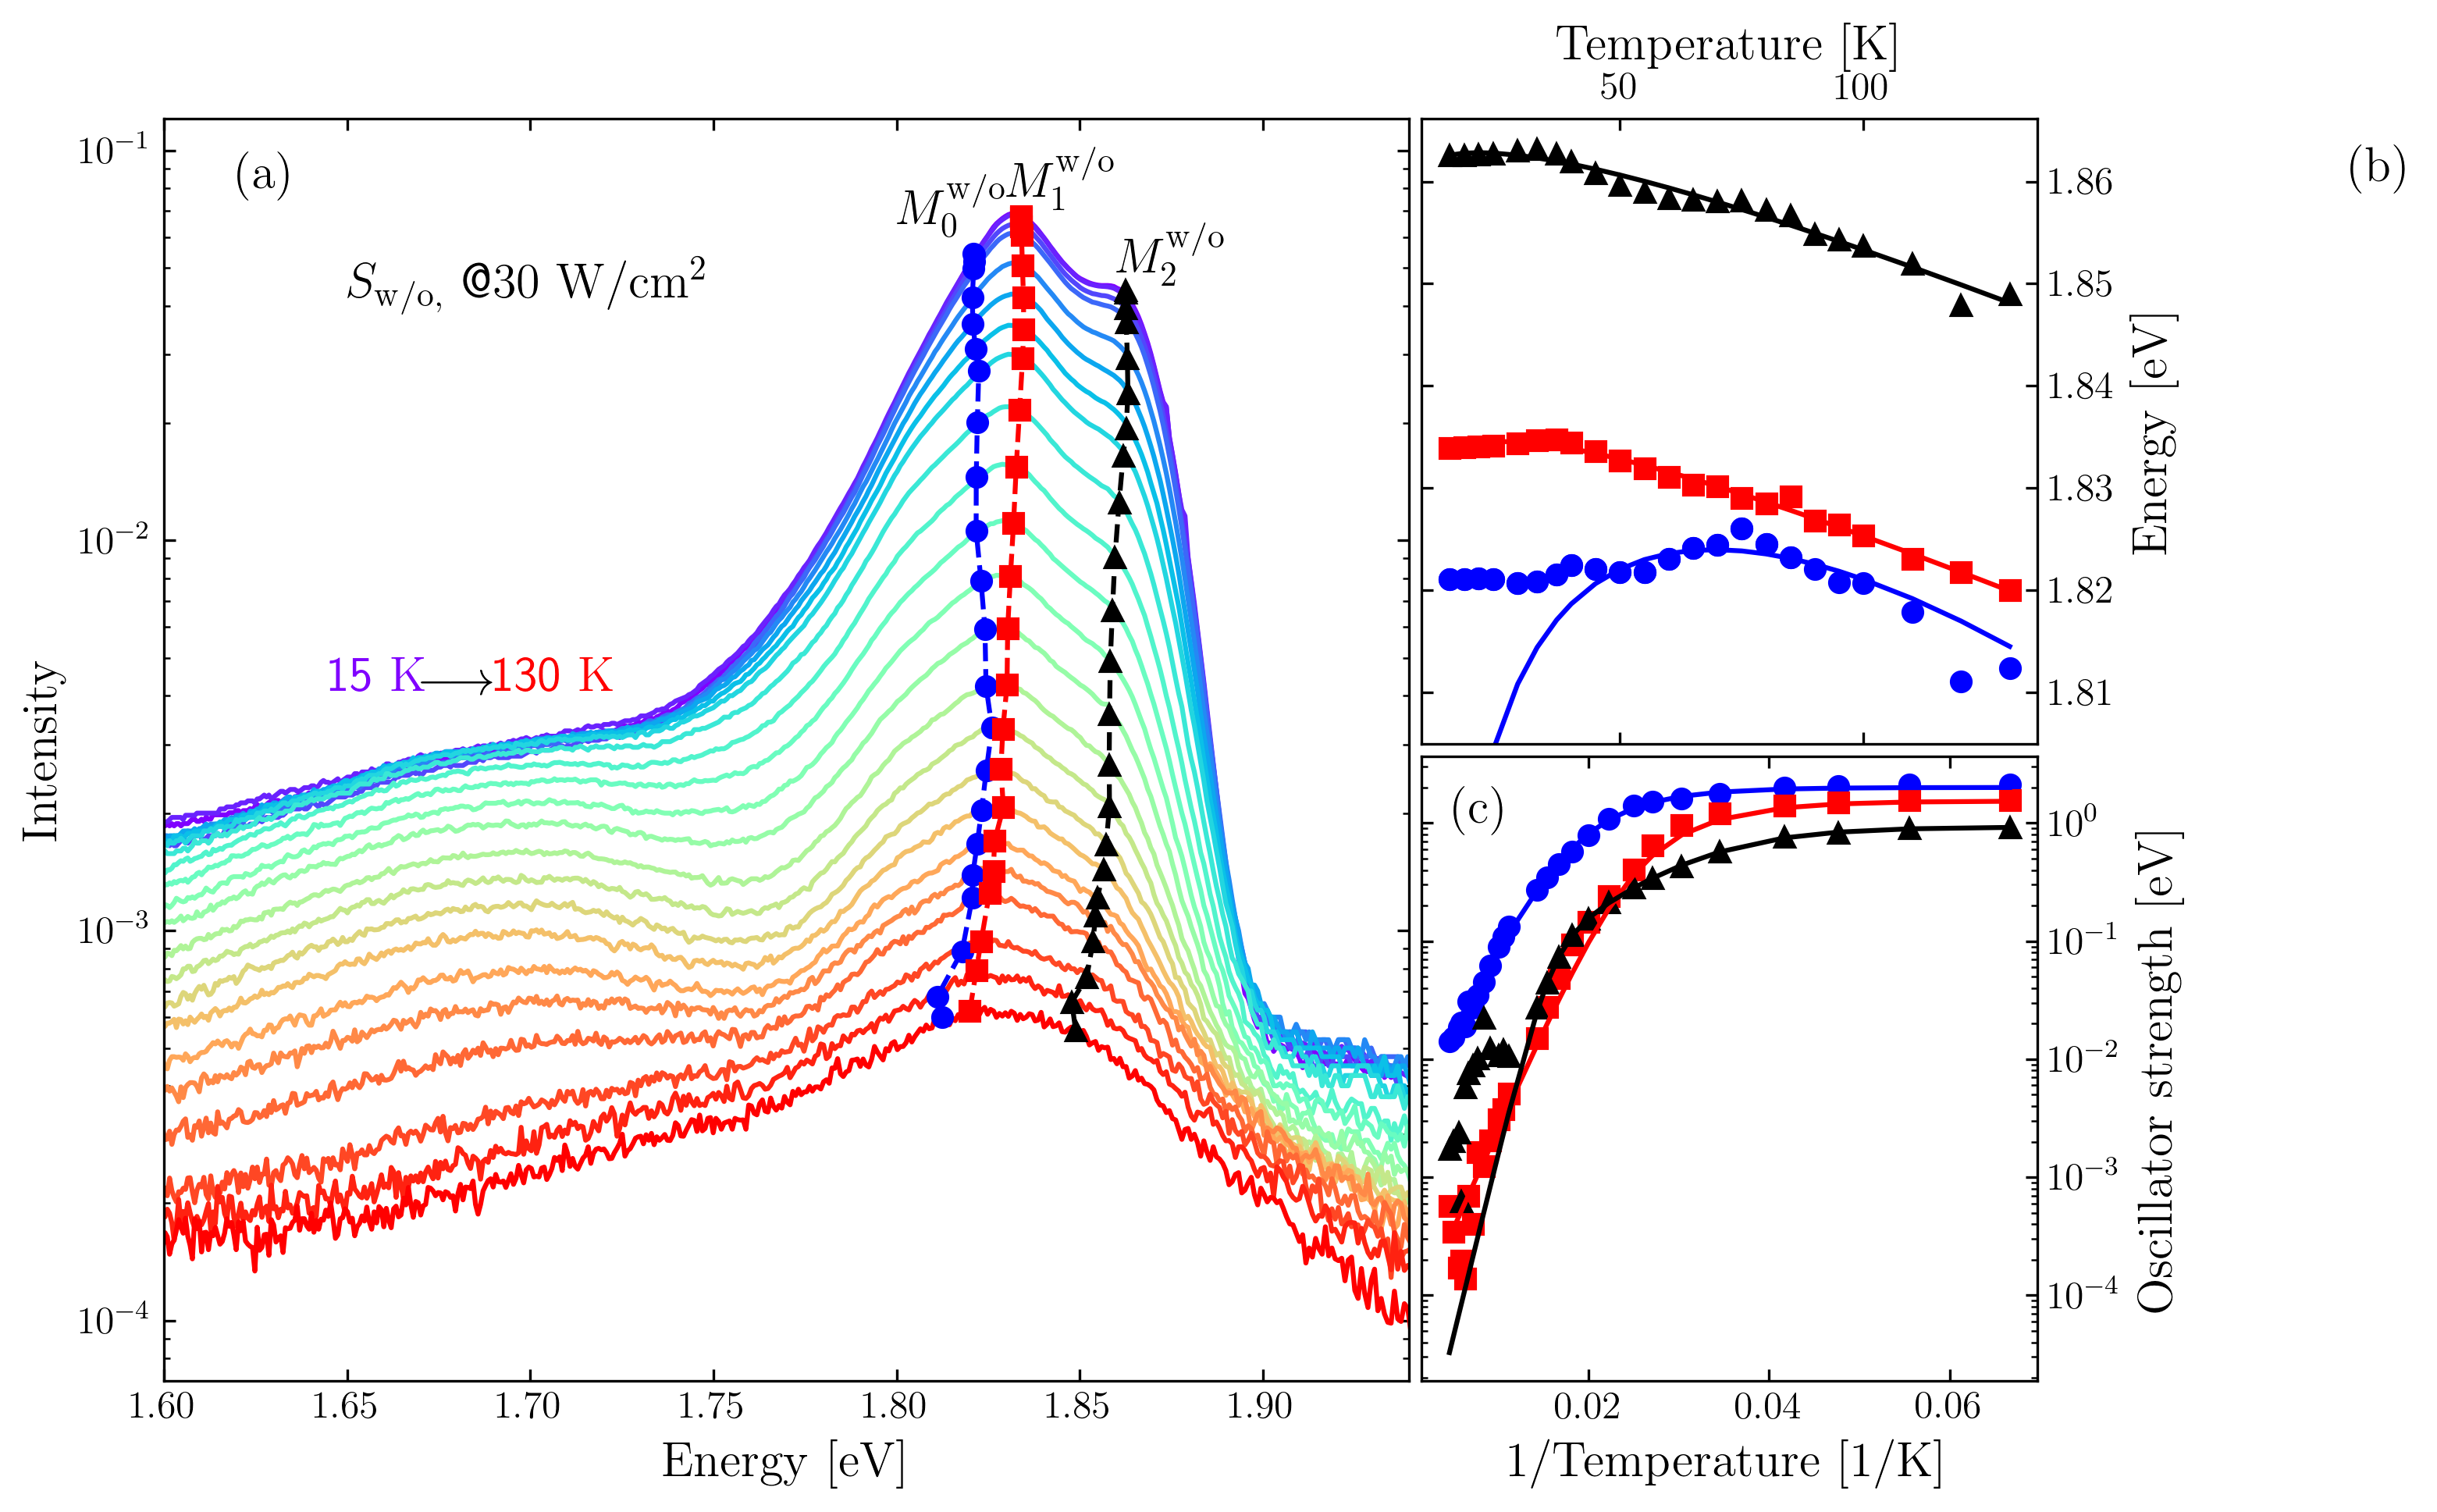
\includegraphics[width=0.9\linewidth]{/PL/temperature/12027_7mW_log_PL_int_without}
	\caption{(a) PL spectra of sample $S_\mathrm{w/o}$ measured at 30~W/cm$^2$ excitation density in 15-220~K temperature range. Each spectrum is fitted by a sum of three Gaussian profiles represented by symbols in panel (a): $M_0^\mathrm{w/o}$ blue circles, $M_1^\mathrm{w/o}$ red squares and $M_2^\mathrm{w/o}$ black triangles. The bands are similarly marked in panels (b) and (c) where also the experimental transition energies (symbols) and fits by the Varshni model~(\ref{eq:Varshni-like}) (lines), respectively, and the integrated PL intensity (symbols) fitted by the Boltzmann model~Eq.~(\ref{eq:Arhenius}) are presented. All fitting parameters are listed in Tabs.~\ref{tab:Varshni} and~\ref{tab:Arhenius}.}
	\label{fig:QD_wo_temp}
\end{figure}


\subsubsection*{Sample with QDs $\mathbf{S_\mathrm{with}}$}
%
In temperature range between 15 and 150~K we observe quenching of PL intensity of three optical transitions marked $M_0^\mathrm{w}$, $M_1^\mathrm{w}$ and $M_2^\mathrm{w}$, see Fig.~\ref{fig:QD_w_temp}(a). The transition energies (Fig.~\ref{fig:QD_w_temp}(b)) and the oscillator strengths (Fig.~\ref{fig:QD_w_temp}(c)) are fitted by the Varshni model~Eq.~(\ref{eq:Varshni-like}) and the Boltzmann model~Eq.~(\ref{eq:Arhenius}) in the whole measured temperature range.  
%
\begin{figure}
	\centering
	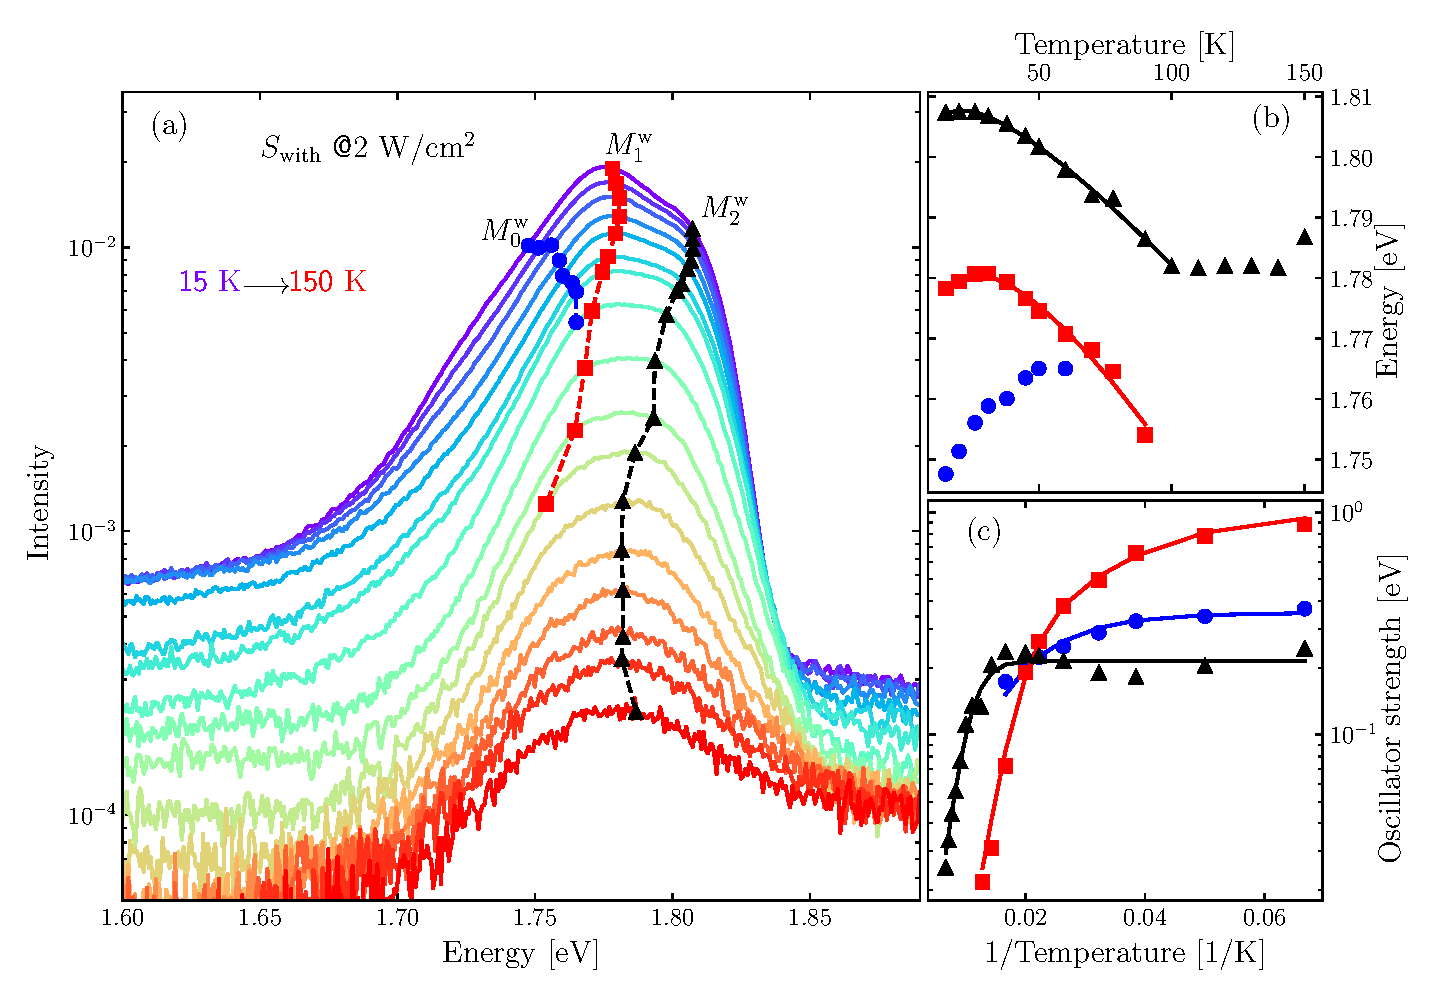
\includegraphics[width=0.9\linewidth]{/PL/temperature/12040_500uW_log_PL_int_Varshni}
	\caption{PL spectra of the sample ${S_\mathrm{with}}$ at 2~W/cm$^2$ between 15 and 150~K. The results are given in the same way as in Fig.~\ref{fig:QD_wo_temp}.}
	\label{fig:QD_w_temp}
\end{figure}

\newpage
\subsubsection*{Sample with capped QDs $\mathbf{S_\mathrm{cap}}$}
%
PL spectra of ${S_\mathrm{cap}}$ are deconvolved into three bands ($M_0^\mathrm{c}$, $M_1^\mathrm{c}$ and $M_2^\mathrm{c}$) and investigated in temperature range 15-110~K, see Fig.~\ref{fig:QD_c_temp}.
%
\begin{figure}[h]
	\centering
	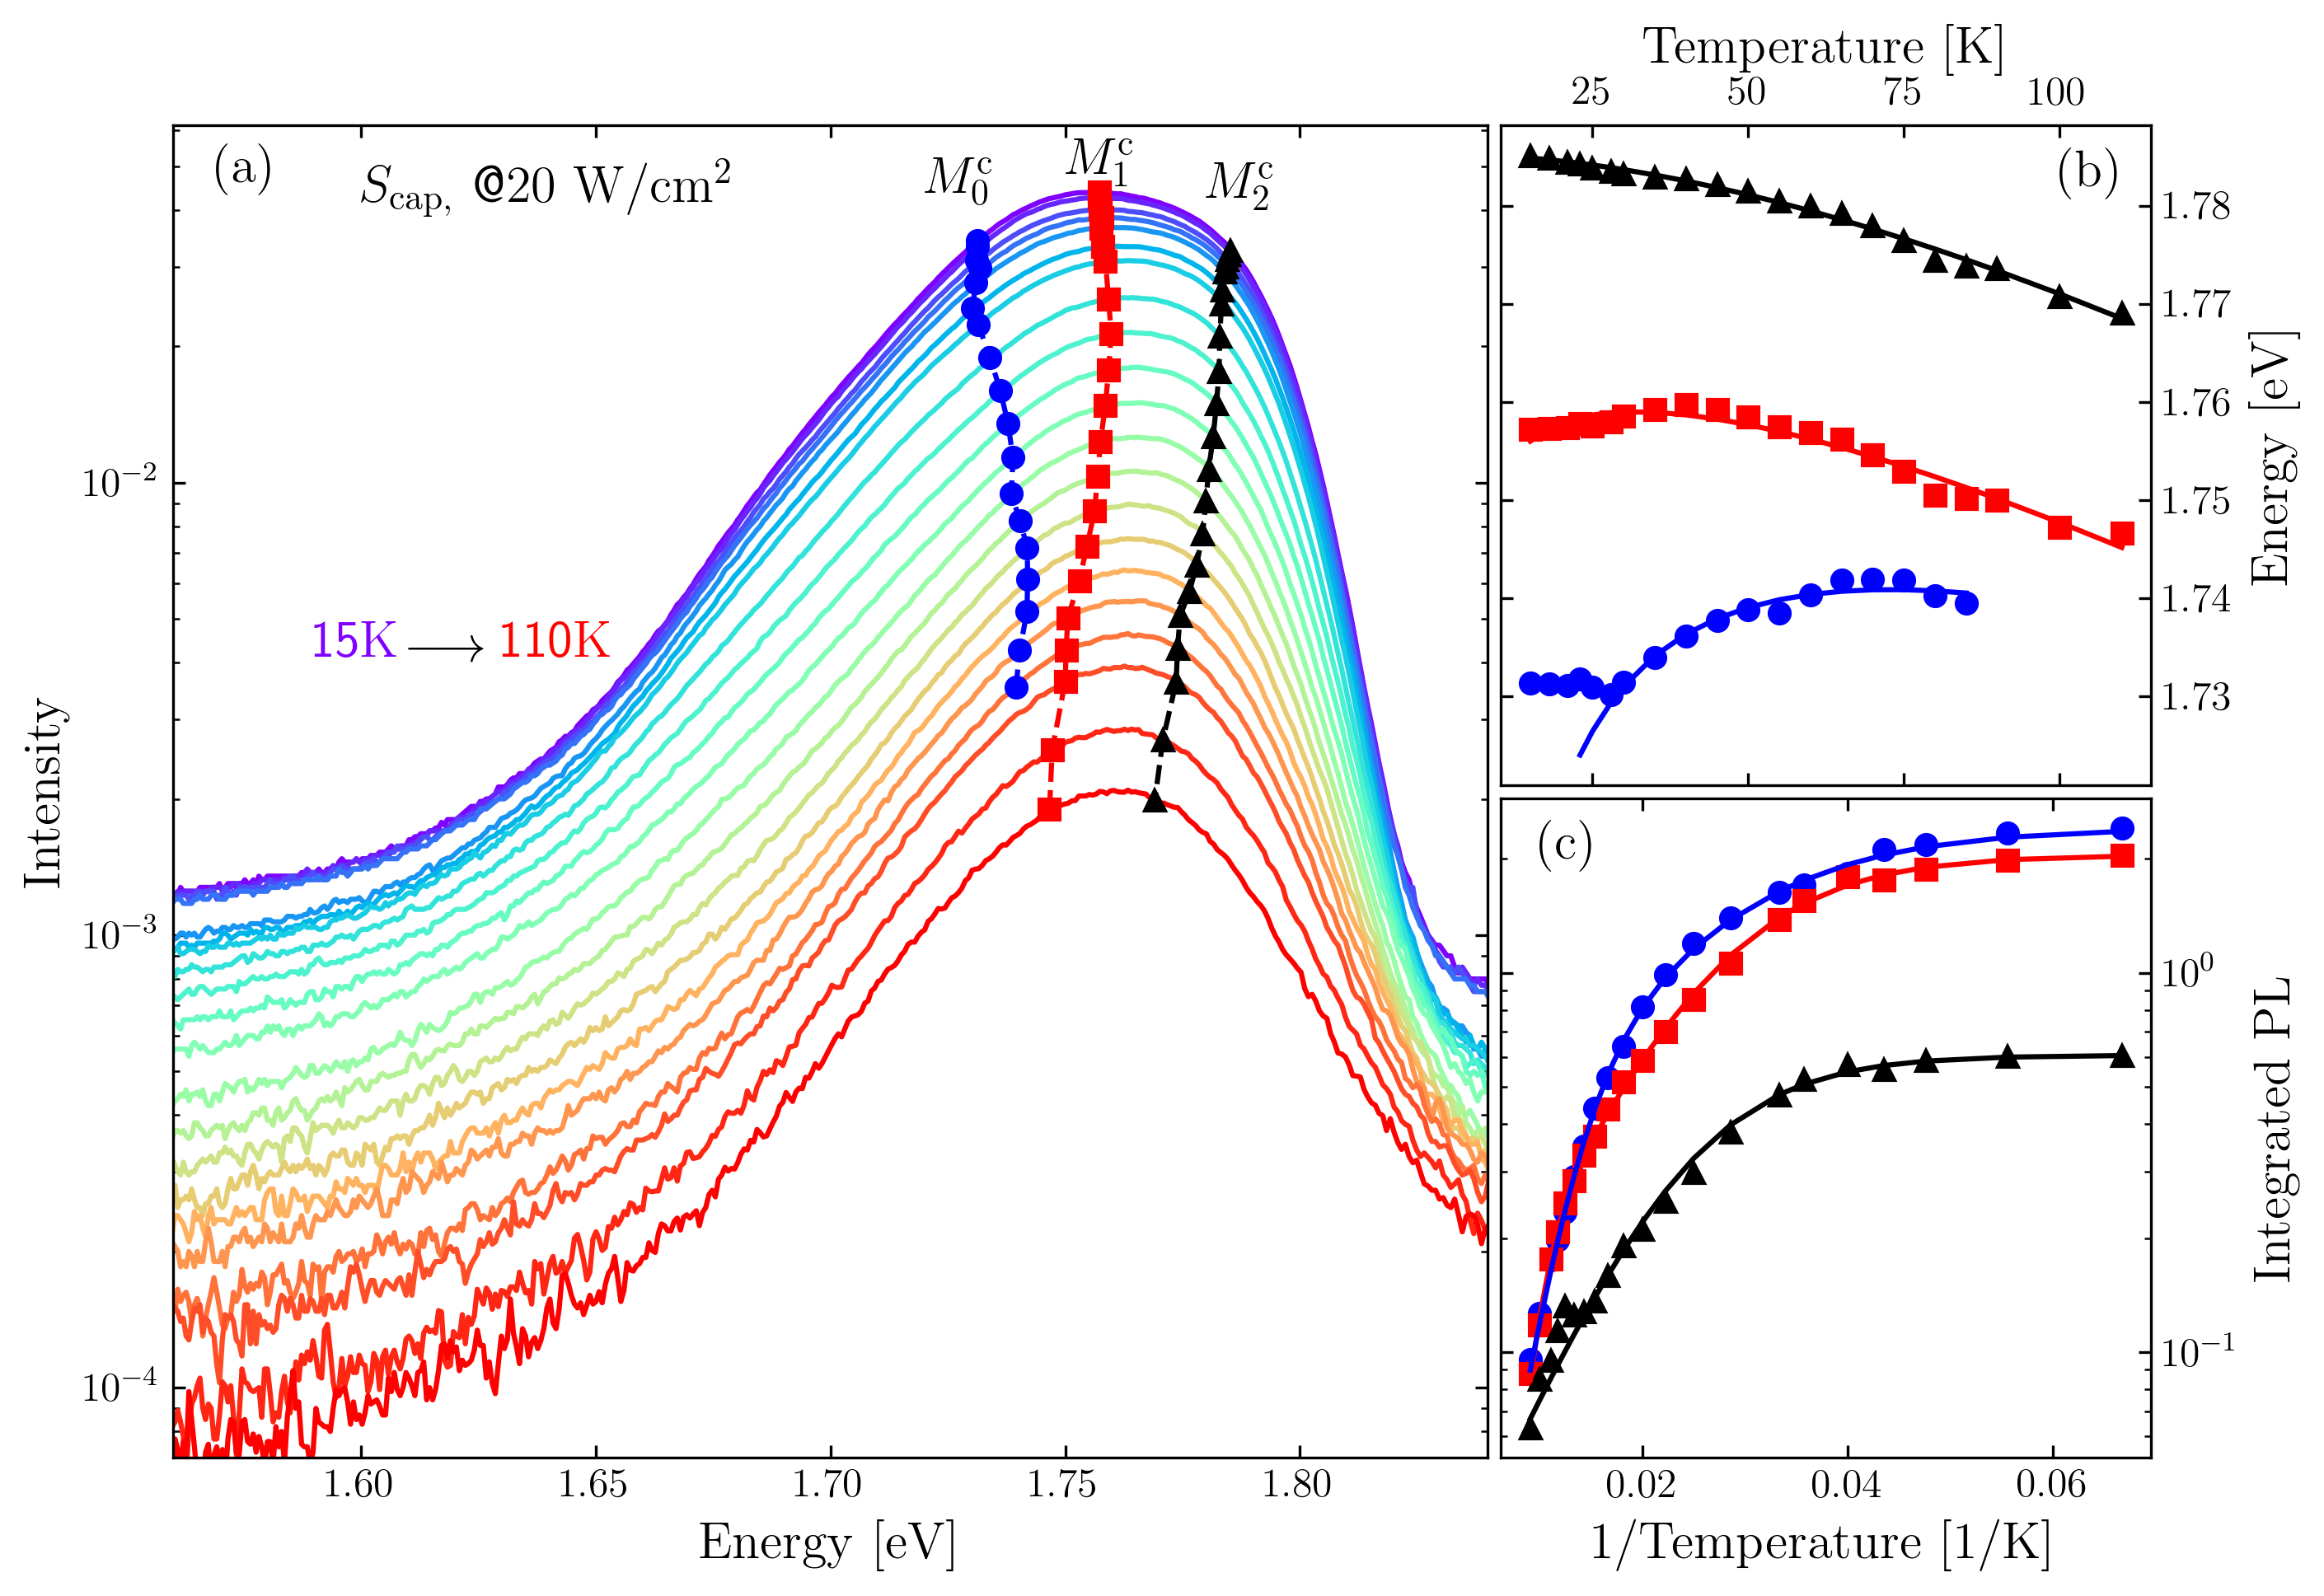
\includegraphics[width=0.9\linewidth]{/PL/temperature/12021_5mW_log_PL_int_Varshni}
	\caption{PL spectra of the sample ${S_\mathrm{cap}}$ measured at 20~W/cm$^2$ between 15 and 110~K. The results are given in the same nomenclature as in Fig.~\ref{fig:QD_wo_temp}.}
	\label{fig:QD_c_temp}
\end{figure}

\newpage
\subsubsection*{Discussion of temperature resolved PL results}
The value of $E_1$ (4--15~meV) is comparable for all samples and also for every PL bands. This low activation energy is determining the low-temperature quenching of the PL and it is usually associated to carrier recombination through impurities. The values of the high-temperature quenching $E_2$ (29--43~meV) are also similar across the samples except the deviation in $M_2^\mathrm{c}$ where we measured extremely small activation energy ($E_2=1$~meV) and $M_2^\mathrm{w/o}$ with $E_2$ twice larger than for other bands ($E_2=62$~meV).

\begin{figure}
	\centering
	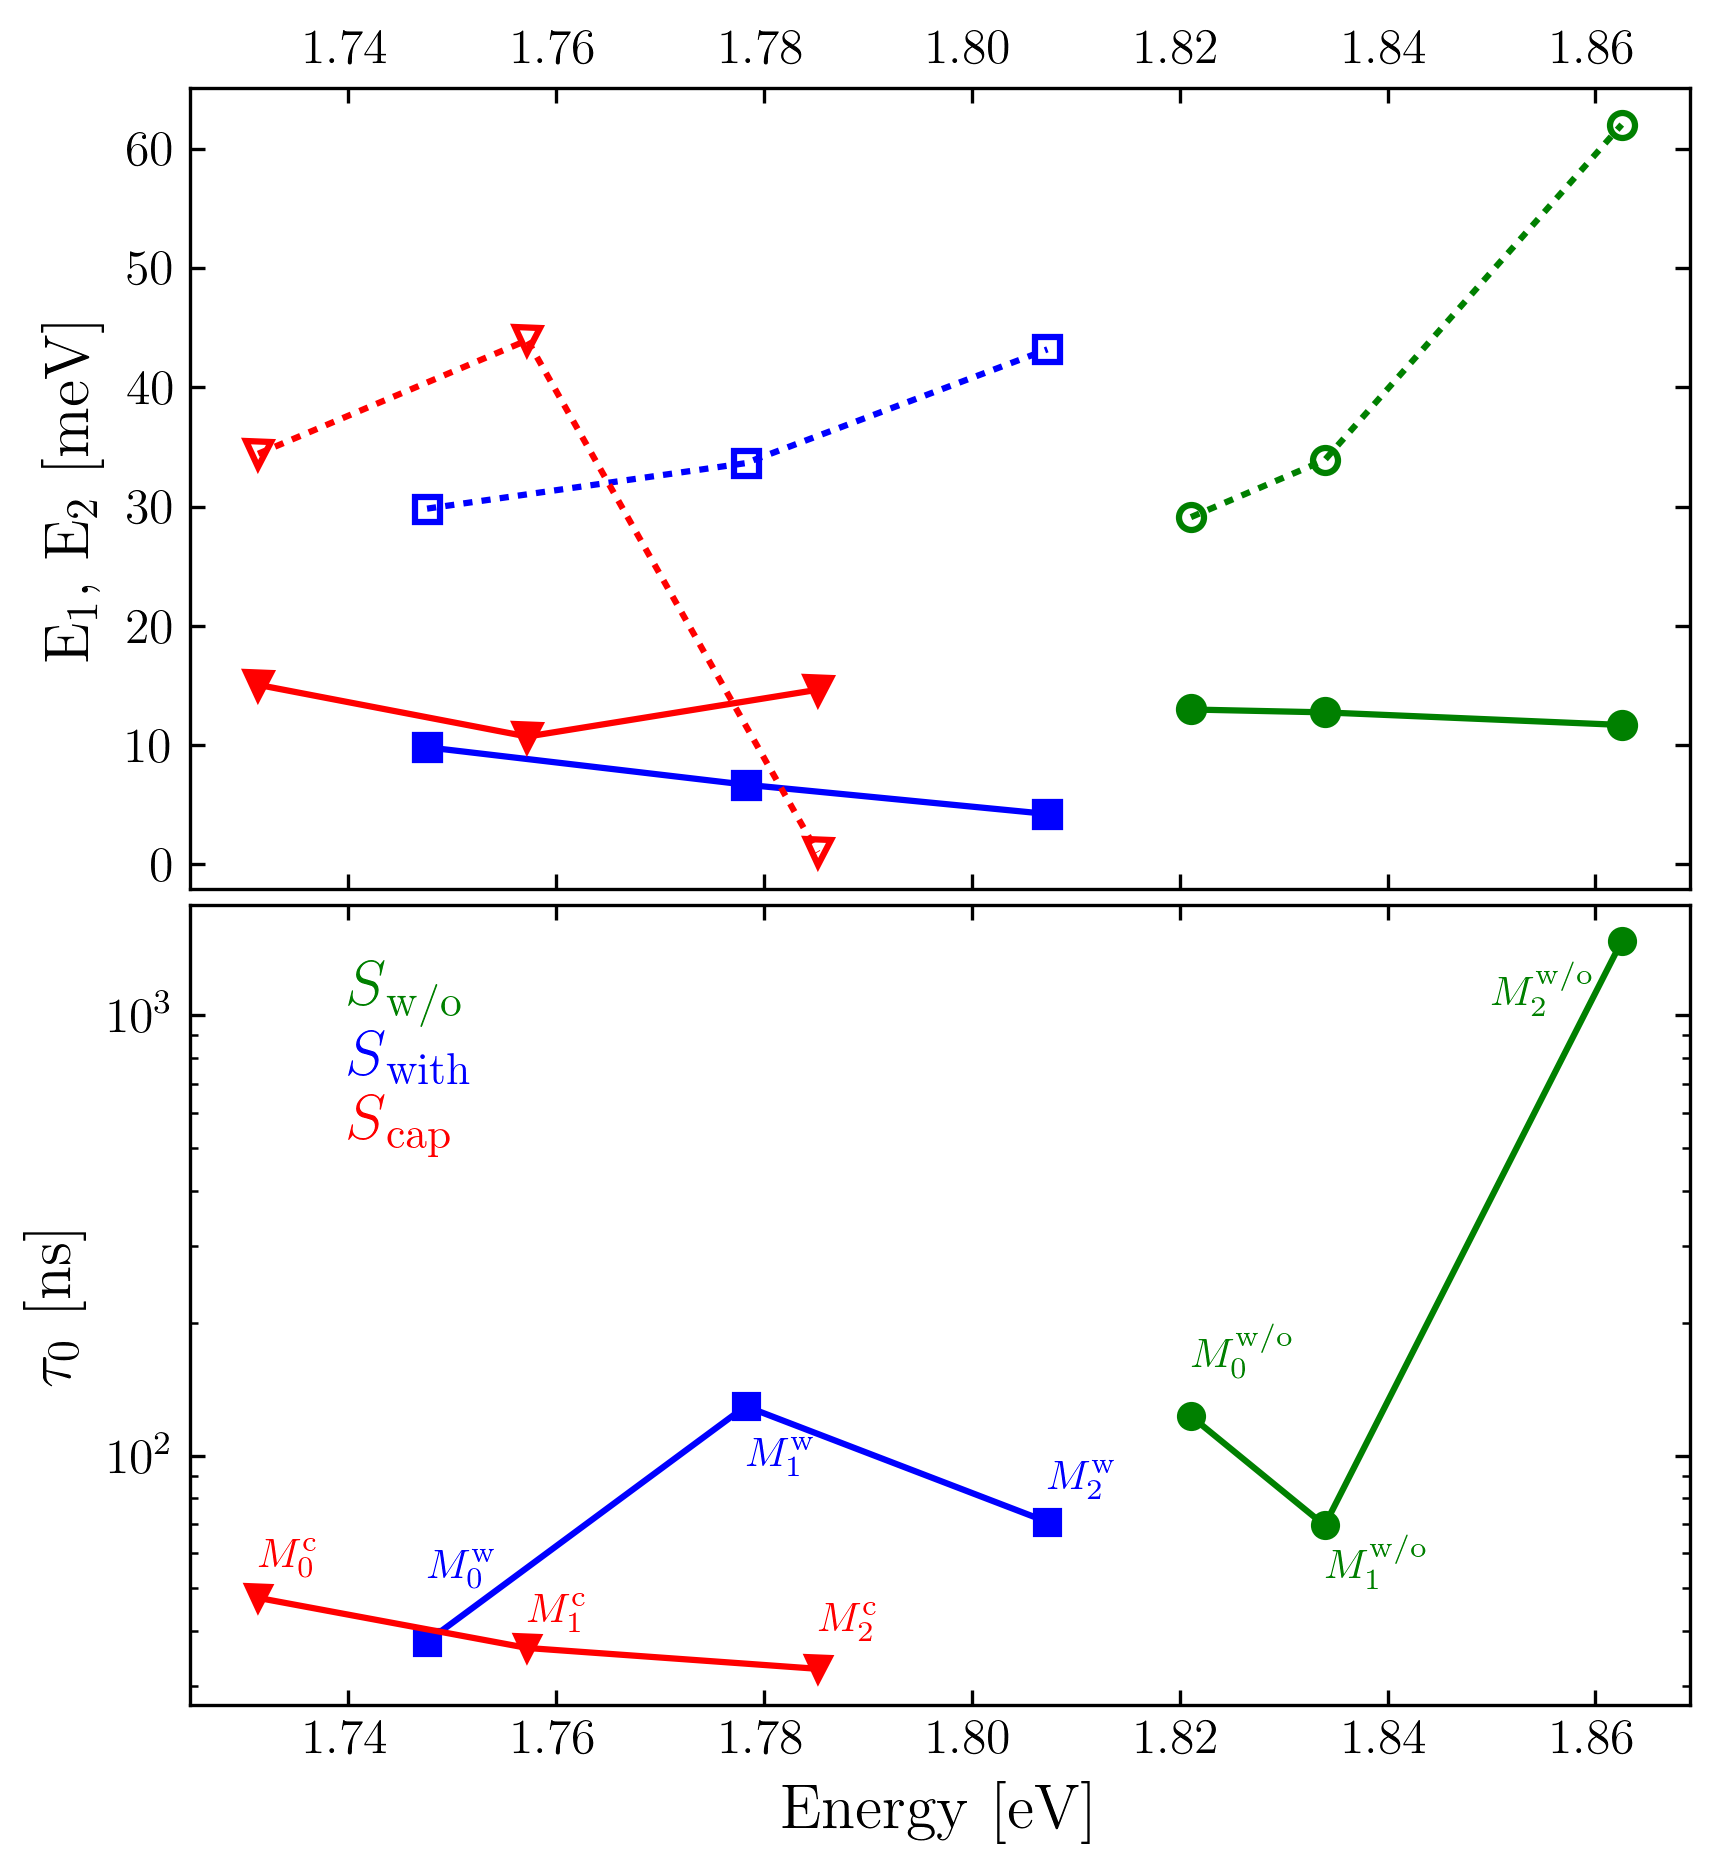
\includegraphics[width=0.75\linewidth]{/PL/temperature/all_Arhenius}
	\caption{Comparison of the Boltzmann fitting parameters for the studied samples. The upper panel depicts $E_1$ (empty symbols) and $E_2$ (full symbols), respectively, the bottom panel shows $\tau_0$. Samples are distinguished by the type and colour of symbols as in Fig.~\ref{fig:PL_homogenity}.}
	\label{fig:Arrhenius_all}
\end{figure}


\begin{table}
	\centering
	\caption{Summary of the Varshni-like fits. The accuracy of $E_0$ and $\alpha$ are better than $10^{-4}\%$, and better than 5~\% for $\Theta_\mathrm{D}$ and $\sigma$.}
	\begin{tabularx}{0.9\textwidth}{cCCcc}
		\toprule
		
		transition & $E_0$ [meV]& $\alpha$ [$10^{-4}~\mathrm{eVK^{-1}}$]& $\Theta_\mathrm{D}$ [K]& $\sigma$ [meV]\\ 	
		\midrule
		\midrule
		$M_0^\mathrm{w/o}$& - & -& -&-\\
		$M_1^\mathrm{w/o}$& $1841$ & $1.69$& $11.2$&$2.6$\\
		$M_2^\mathrm{w/o}$ & $1868$ & $1.61$& $11.6$& $2.5$\\ 
		
		\midrule
		$M_0^\mathrm{w}$& - & -& -&-\\
		$M_1^\mathrm{w}$& $1792$ & $9.99$& $150.1$&$4.0$\\
		$M_2^\mathrm{w}$ & $1815$& $5.49$& $74.5$& $2.8$\\ 
		
		\midrule
		$M_0^\mathrm{c}$& - & -& -&-\\
		$M_1^\mathrm{c}$& $1766$ & $4.03$& $144.5$& $3.4$\\
		$M_2^\mathrm{c}$ & $1785$ & $4.90$& $243.2$& $3.3\cdot 10^{-7}$\\
		
		\bottomrule
	\end{tabularx}\label{tab:Varshni}
\end{table}

\begin{table}
	\centering
	\caption{Summary of the Arhenius-like fits. The displayed values are obtained with accuracy better than $10^{-4}~\%$.}
	\begin{tabularx}{0.9\textwidth}{cCCcccc}
		\toprule
		
		%transition & $I_0$ & $\tau_0$ [ns]& $\Gamma_1$ [ns$^{-1}$]& $E_1$ [meV]& $\Gamma_2$ [ns$^{-1}$]& $E_2$ [meV]\\ 	
	%	\midrule
	%	\midrule
	%	$M_0^\mathrm{w/o}$& 7.65135744e-01&   65.2916823&   566.317577&  7.60337981&8.65963570&   27.3857198 \\
	%	$M_1^\mathrm{w/o}$& 4.38191968e-01&   92.4725944&   1.26183745&   15.1174840&   500.994206&   37.1135443\\
	%	$M_2^\mathrm{w/o}$ & 1.00415726e-11&   95.1667043&   34.0939008&   9.27548824&   96.6322136&   36.5620565\\ 
		
	%	\midrule
	%	$M_0^\mathrm{w}$& 3.53321027e-01&   37.8298857&   17.4314590&  9.81156539&   2.85772107 &  29.8347168\\
	%	$M_1^\mathrm{w}$& 9.99521298e-01 &  129.480243 &  864.188777 &  6.67625574&   39.7837356 &  33.6514094\\
	%	$M_2^\mathrm{w}$ & 2.15529619e-01&   70.7125983&   297.344867 &  4.21713415&   25.0223987 &  43.1983367\\ 
		
	%	\midrule
	%	$M_0^\mathrm{c}$& 2.40563456e+00&  47.5372923&   4.03965001&  34.4371546&   1.38672287&   15.0504481\\
	%	$M_1^\mathrm{c}$& 2.05316367e+00&   36.5787466&   81.4268881&   10.7120315&   19.2461237&  43.9676048\\
	%	$M_2^\mathrm{c}$ & 2.61200307e+00&   32.8025509 &  18.6448452 &  1.00000016&   5.01856897&  14.6371152\\
		
		
			transition & $I_0$ & $\tau_0$ [ns]& $\Gamma_1$ [ns$^{-1}$]& $E_1$ [meV]& $\Gamma_2$ [ns$^{-1}$]& $E_2$ [meV]\\ 	
			\midrule
			\midrule
			$M_0^\mathrm{w/o}$&  2.000 &  122.9&   13.17&  13.0&  4.62&   29.1 \\
			$M_1^\mathrm{w/o}$& 1.533&   69.5&  93.62&   12.7&   424.25&  33.9\\
			$M_2^\mathrm{w/o}$ &  0.925 &  1474.1 &  456.81 &  11.7&   506.20 &  62.1\\ 
			
			\midrule
			$M_0^\mathrm{w}$& 0.353&   37.8&   17.43&  9.8&   2.86 &  29.8\\
			$M_1^\mathrm{w}$& 0.999 &  129.5 &  864.19&  6.7&   39.78 &  33.7\\
			$M_2^\mathrm{w}$ & 0.216&   70.7&   297.34 &  4.2&   25.02&  43.2\\ 
			
			\midrule
			$M_0^\mathrm{c}$& 2.406&  47.5&   1.39&   15.0 &   4.04&  34.4\\
			$M_1^\mathrm{c}$& 2.053&   36.5&   81.43&   10.7&   19.25&  44.0\\
			$M_2^\mathrm{c}$ & 2.612&   32.8&   5.02&  14.6 &  18.65 &  1.0\\
			
		\bottomrule
	\end{tabularx}\label{tab:Arhenius}
\end{table}


\clearpage
\subsection{Polarization dependent PL }
In our experiments, both the excitation and the detected PL radiation propagate perpendicularly to the sample surface; the angle between the crystallographic direction~[110] and the polarization vector is denoted $\theta$. Because low degrees of polarization of the emitted light is expected, we visualize our experimental results in terms of the degree of polarization
%
\begin{equation}
C(\theta)=\frac{I(\theta)-I_\mathrm{min}}{I_\mathrm{max}+I_\mathrm{min}},
\end{equation}
%
where $I_\mathrm{min}$ and $I_\mathrm{max}$ are extremal values of $I(\theta)$. Note that for angle $\theta_\mathrm{max}$, such that $I(\theta_\mathrm{max})=I_\mathrm{max}$, the previous relation gives the maximum obtained degree of polarization $C(\theta_\mathrm{max})=C_\mathrm{max}$ (values in the polar graphs~\ref{fig:PL_pol_all}).

Non-polarized PL of GaAs layer on sample ${S_\mathrm{with}}$ is expected, therefore we are using degree of polarization of $M_1^\mathrm{w/o}$ to re-calibrate degree of polarization of other bands to eliminate the residual polarization of the whole setup. The calibrated $C(\theta)$ of individual bands are plotted in Fig.~\ref{fig:PL_pol_all}. Note that almost no polarization anisotropy is observed on sample ${S_\mathrm{w/o}}$.

The emission radiation of samples containing QDs is polarized along the [110]~crystallographic direction, in agreement with results on type-I InAs/GaAs QDs~\citep{HumPhysE} where the polarization anisotropy of $I(\theta)$ is dictated predominantly by the orientation of the wavefunction of hole states. Based on that noticing the results of Ref.~\citep{Klenovsky2015} we conclude that the studied samples are type-I.

 %The sample ${S_\mathrm{with}}$ has $C_\mathrm{max}$ around 0.04, which is typically observable value on InAs/GaAs QDs, where one-particle wavefunctions are precisely located in the same position in the QD. Sb from GaSb capping on ${S_\mathrm{cap}}$ causes that the wavefunctions move slightly toward each other therefore the polarization anisotropy grows up to almost 0.15.
  The sample ${S_\mathrm{with}}$ has $C_\mathrm{max}$ around 0.04, which is comparable to that for InAs/GaAs QDs where one-particle wavefunctions are located in the same position in the QD. Antimony from GaSb capping in sample ${S_\mathrm{cap}}$ causes that the wavefunctions of electrons and holes are positioned slightly further apart from each other therefore the polarization anisotropy grows up to almost 0.15.
  
\begin{figure}
	\centering
	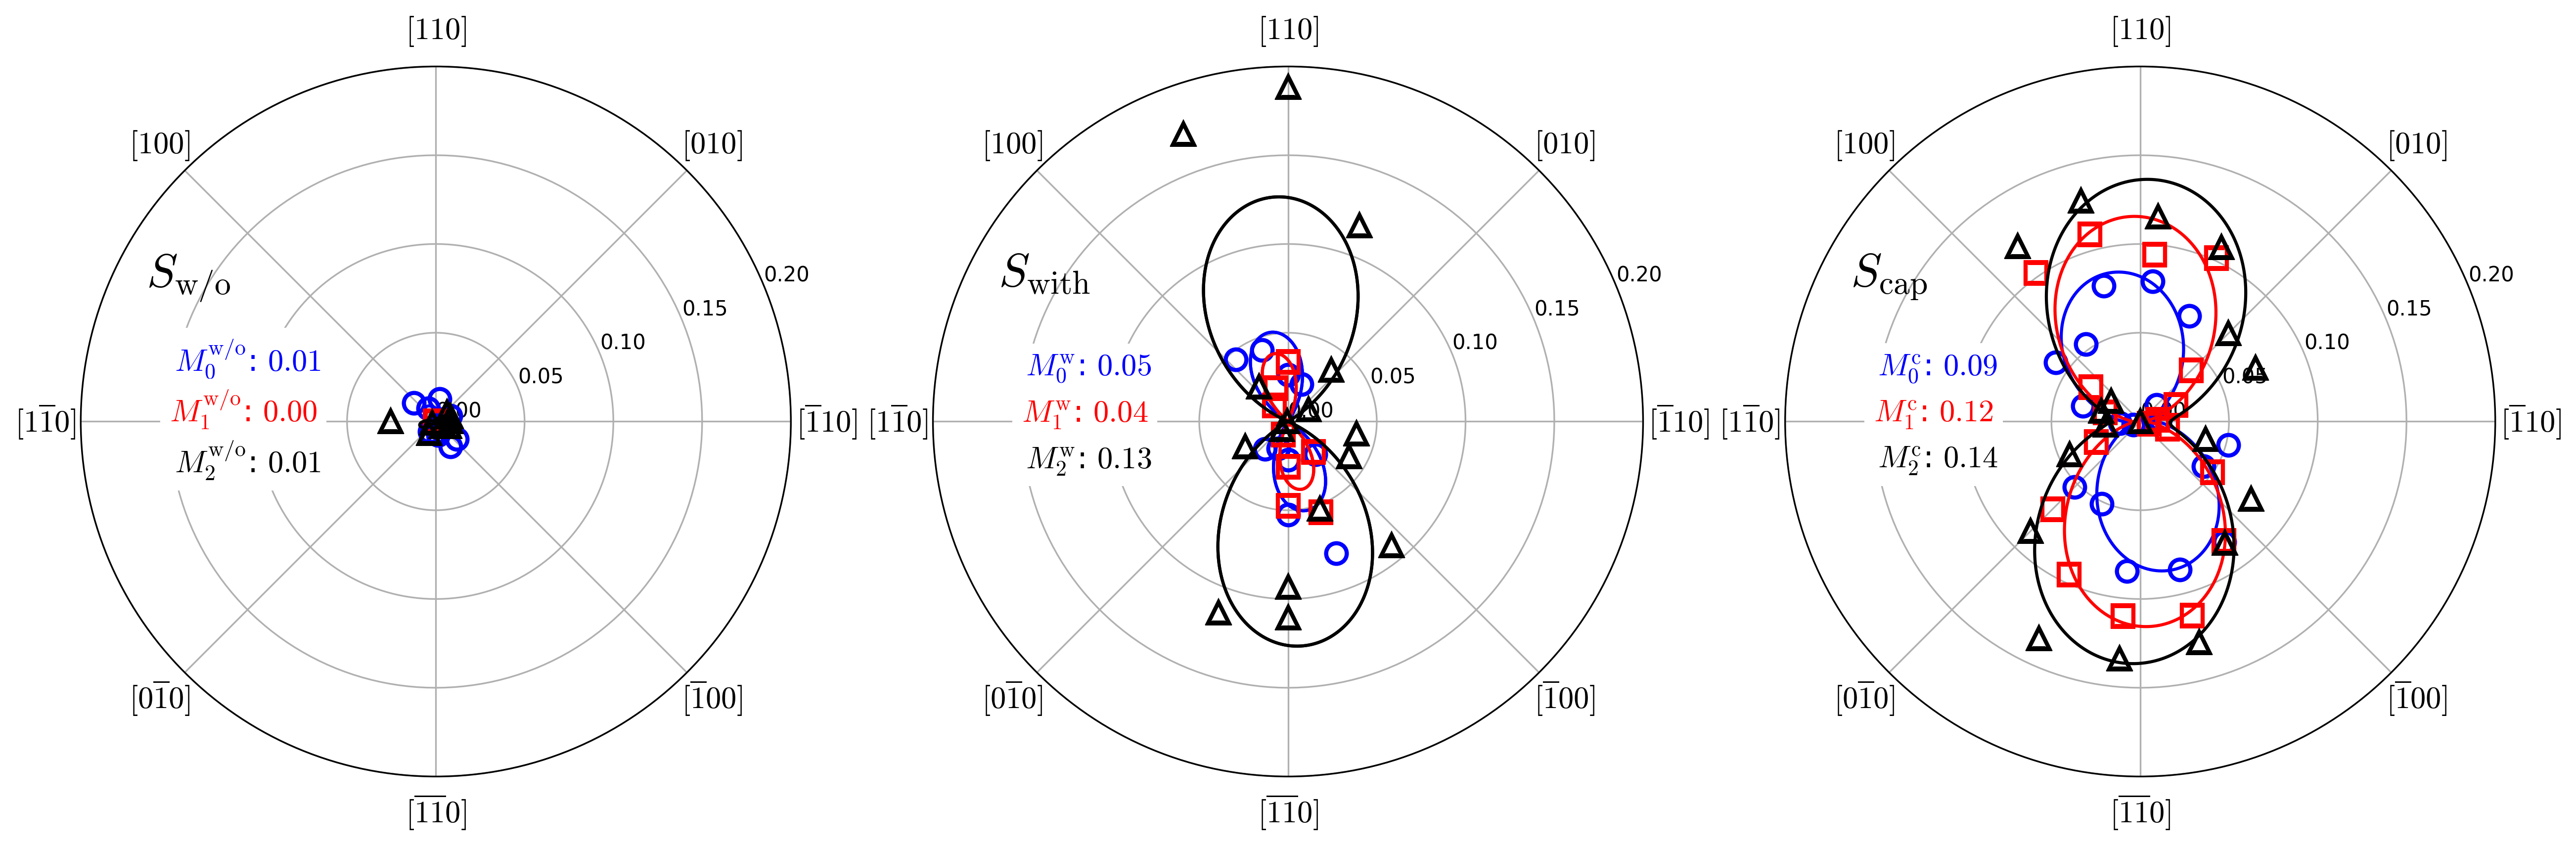
\includegraphics[width=1\linewidth]{/PL/polarization/POL_all}
	\caption{From left to right the polar graphs show $C(\theta)$ of sample ${S_\mathrm{w/o}}$, ${S_\mathrm{with}}$ and $\mathbf{S_\mathrm{cap}}$, respectively. Individual bands of PL spectra for each sample are represented by different symbols, consistently with previous labeling.}
	\label{fig:PL_pol_all}
\end{figure}

\newpage
\section{Time-resolved photoluminiscence}
%The measurements can be fitted to a double exponential decay function after convolution with the instrument response function (IRF) shown in the same graph
We have studied the dynamics of the recombination processes of our QD samples as a function of the emission energy, excitation density, and temperature. Each measured TRPL signal has been deconvoluted using a double mono-exponential (2ME) decay model
\begin{equation}
I(t)=A_1\exp(-t/\tau_1)+A_2\exp(-t/\tau_2),
\end{equation}
 characterized by the amplitude $A_1$ ($A_2$) and the decay time $\tau_1$ ($\tau_2$) for the slow (fast) decay process. In order to compare the samples we introduce characteristic PL decay time $\tau_\mathrm{PL}$ which corresponds to a decrease of PL intensity from its maximum value to the level of $1/\mathrm{e}$:
%
\begin{eqnarray}
\tau_\mathrm{PL}=w_1\tau_1+w_2\tau_2, \label{eq:average_time}
\end{eqnarray}
%
where $w_1$ and $w_2$ are weights (weight: $w_i={A_i\cdot \tau_i }/{(\sum A_i \cdot \tau_i)}$) defined by the 2ME fitting model.

Figure~\ref{fig:TRPL_int_all}(a) summarizes the average decay times measured under the same conditions as a function of the emission energy for all three samples. 
%
\begin{figure}
\centering
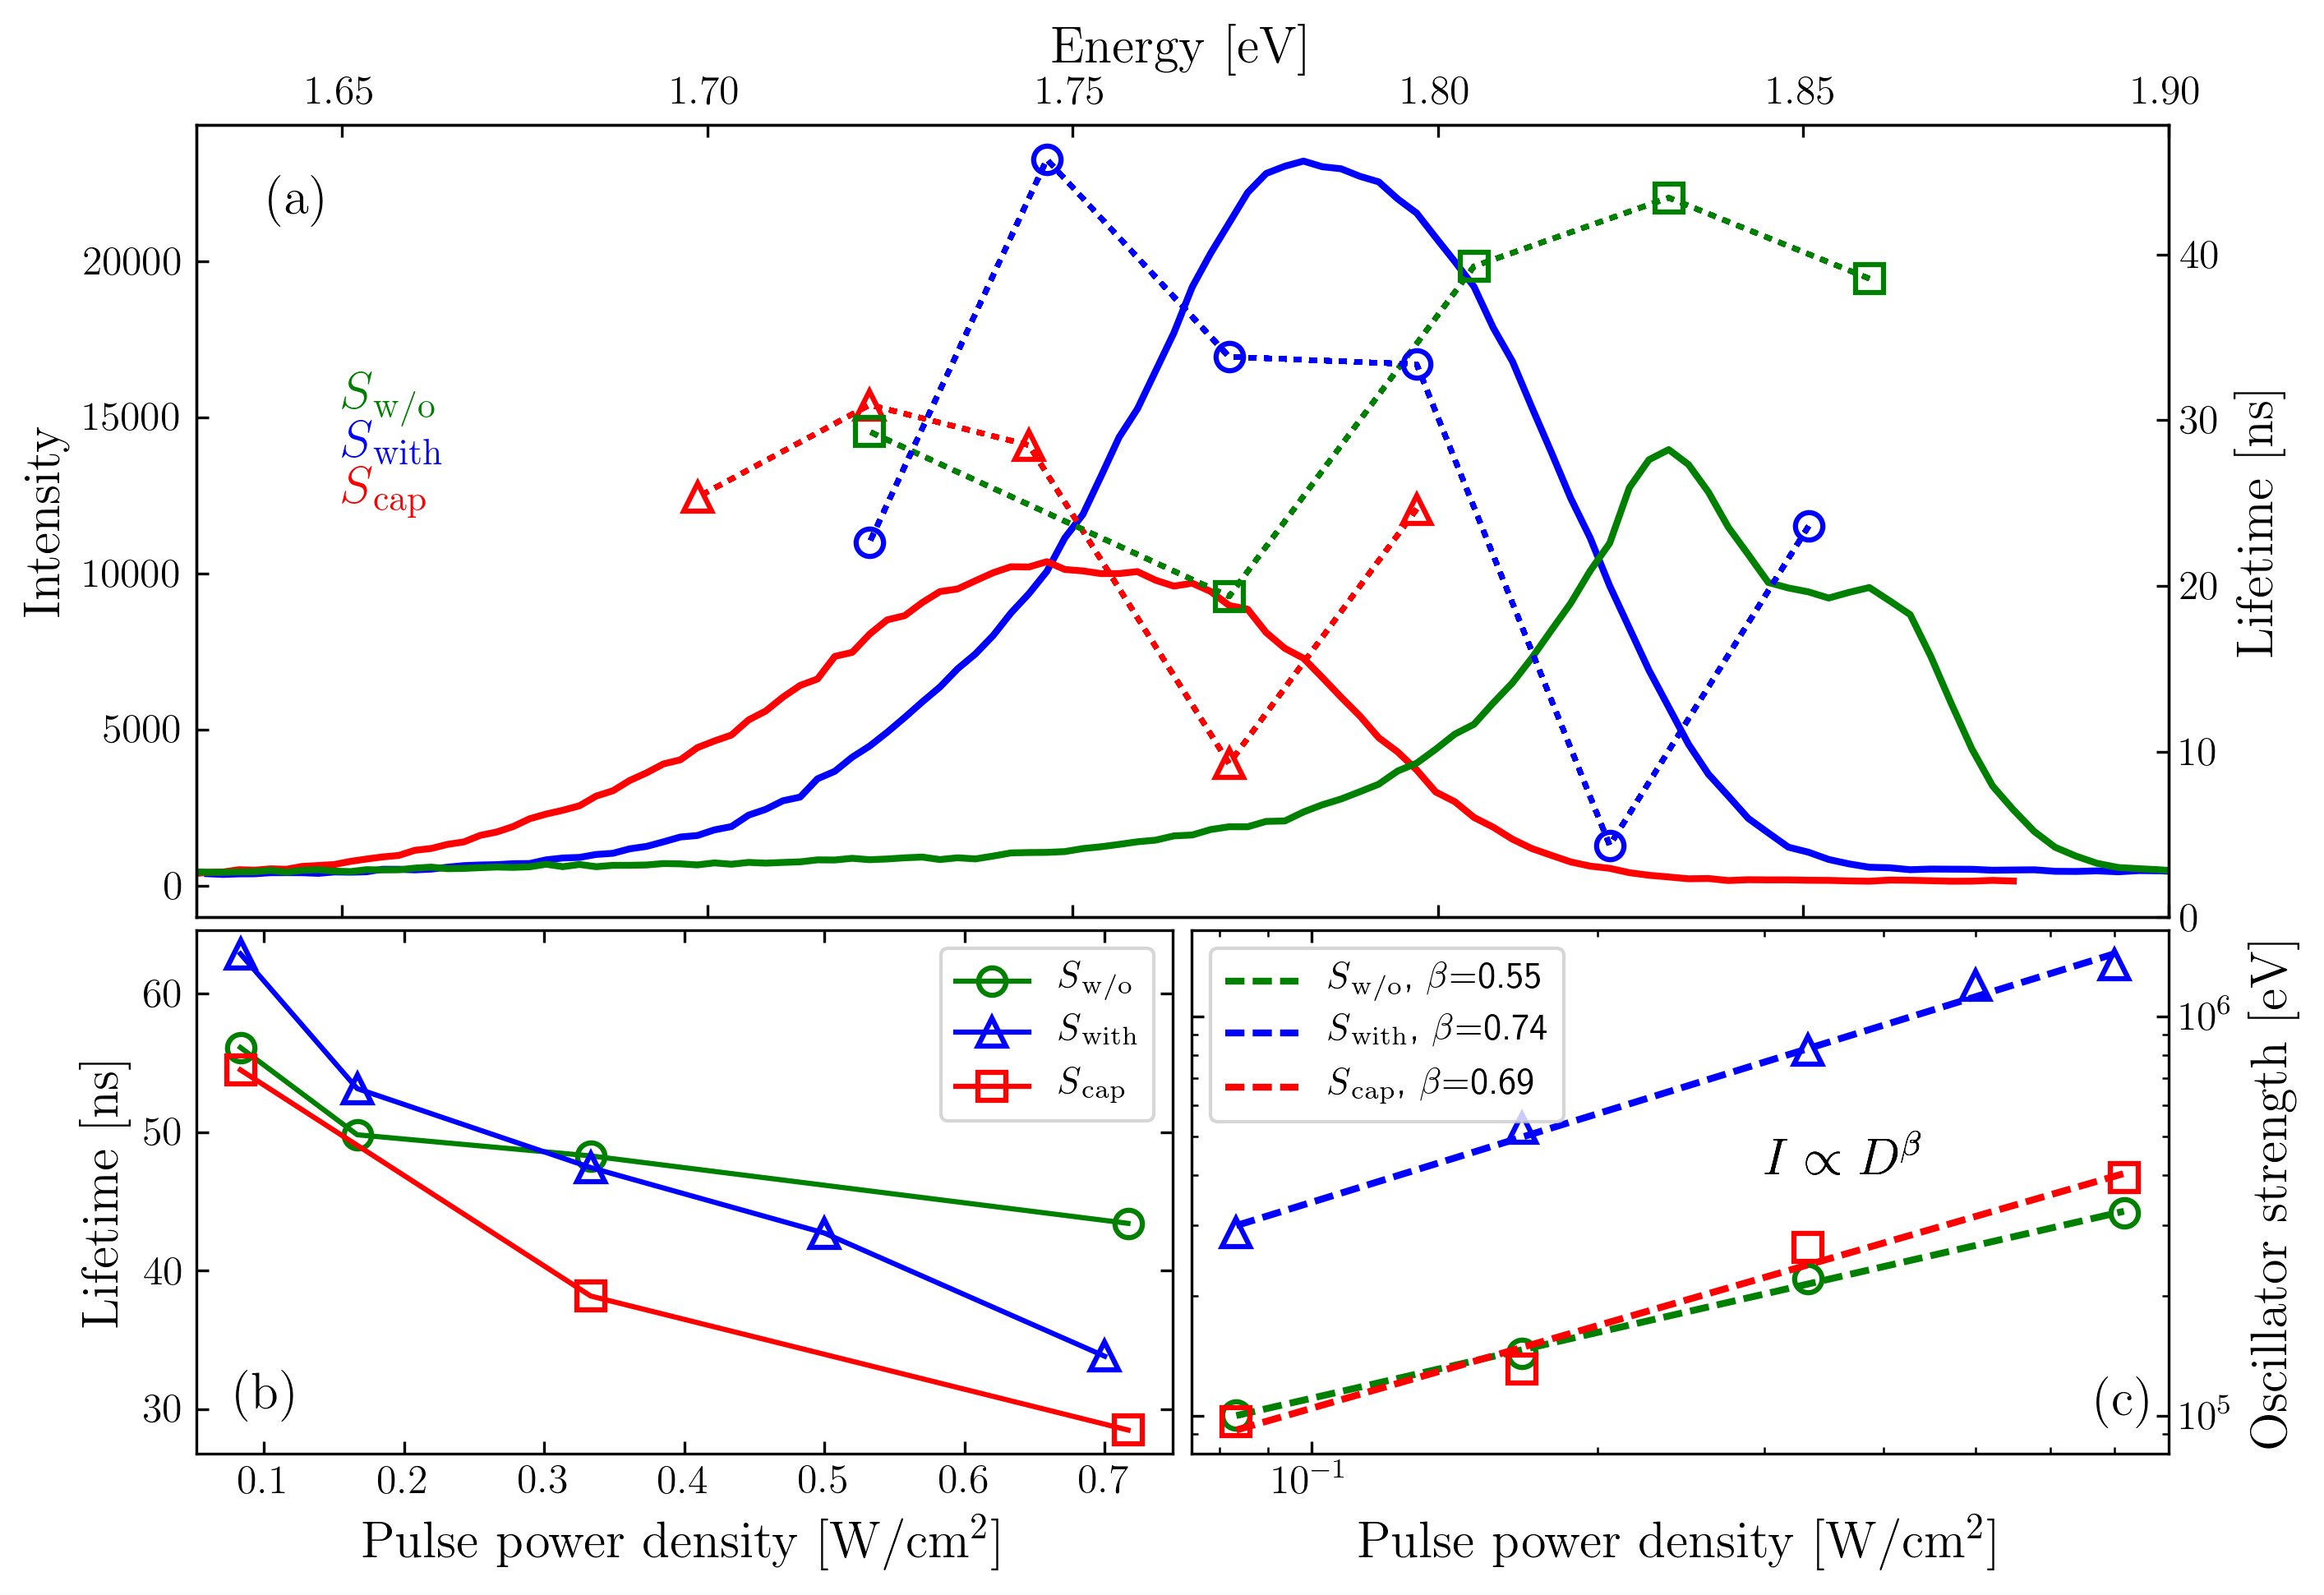
\includegraphics[width=1\linewidth]{/TRPL/intensity/porovnani_vzorku_maximum_int}
\caption{(a) Decay times $\tau_\mathrm{PL}$ (symbols) for the studied samples as a function of the emission energy measured at 15~K and 0.7~W/cm$^2$. Appropriate PL spectra (solid lines) are added for better orientation. Panel~(b) depicts $\tau_\mathrm{PL}$ in the maximum of the PL signal and panel~(c) $\tau_\mathrm{PL}$ for the integrated PL intensity in whole measured range as a function of excitation density for the samples.}
\label{fig:TRPL_int_all}
\end{figure}


\subsection{Excitation intensity dependent TRPL}
The excitation density of the pulse laser was varied in the range 0.08--0.7~W/cm$^2$ (the optical response was in linear regime in the whole varied excitation range for each sample, see Fig.~\ref{fig:TRPL_int_all}(c)), then the measured TRPL signal has been deconvoluted by 2ME decay model, e.~g., Fig.~\ref{fig:TRPL_int_w} depicts TRPL signal in the maximum of PL spectra of $S_\mathrm{with}$). 

We observe a decrease of the fast decay component with increasing excitation density as shown in Fig.~\ref{fig:TRPL_int_w}(b)--(c), which is in agreement with behaviour of type-II nanostructures observed elsewhere~\citep{Ledentsov_prb1995_intmodel,Gu_prb2005_TRPLtype2,Manna_apl2012_TRPLtype2,Zaitsev_prb2007}. At higher excitation intensity, a larger carrier concentration of the photogenerated electron-hole pairs results in band bending, hence a stronger overlap of electron-hole wave-functions, and thus a faster decay.
%

\begin{figure}
	\centering
	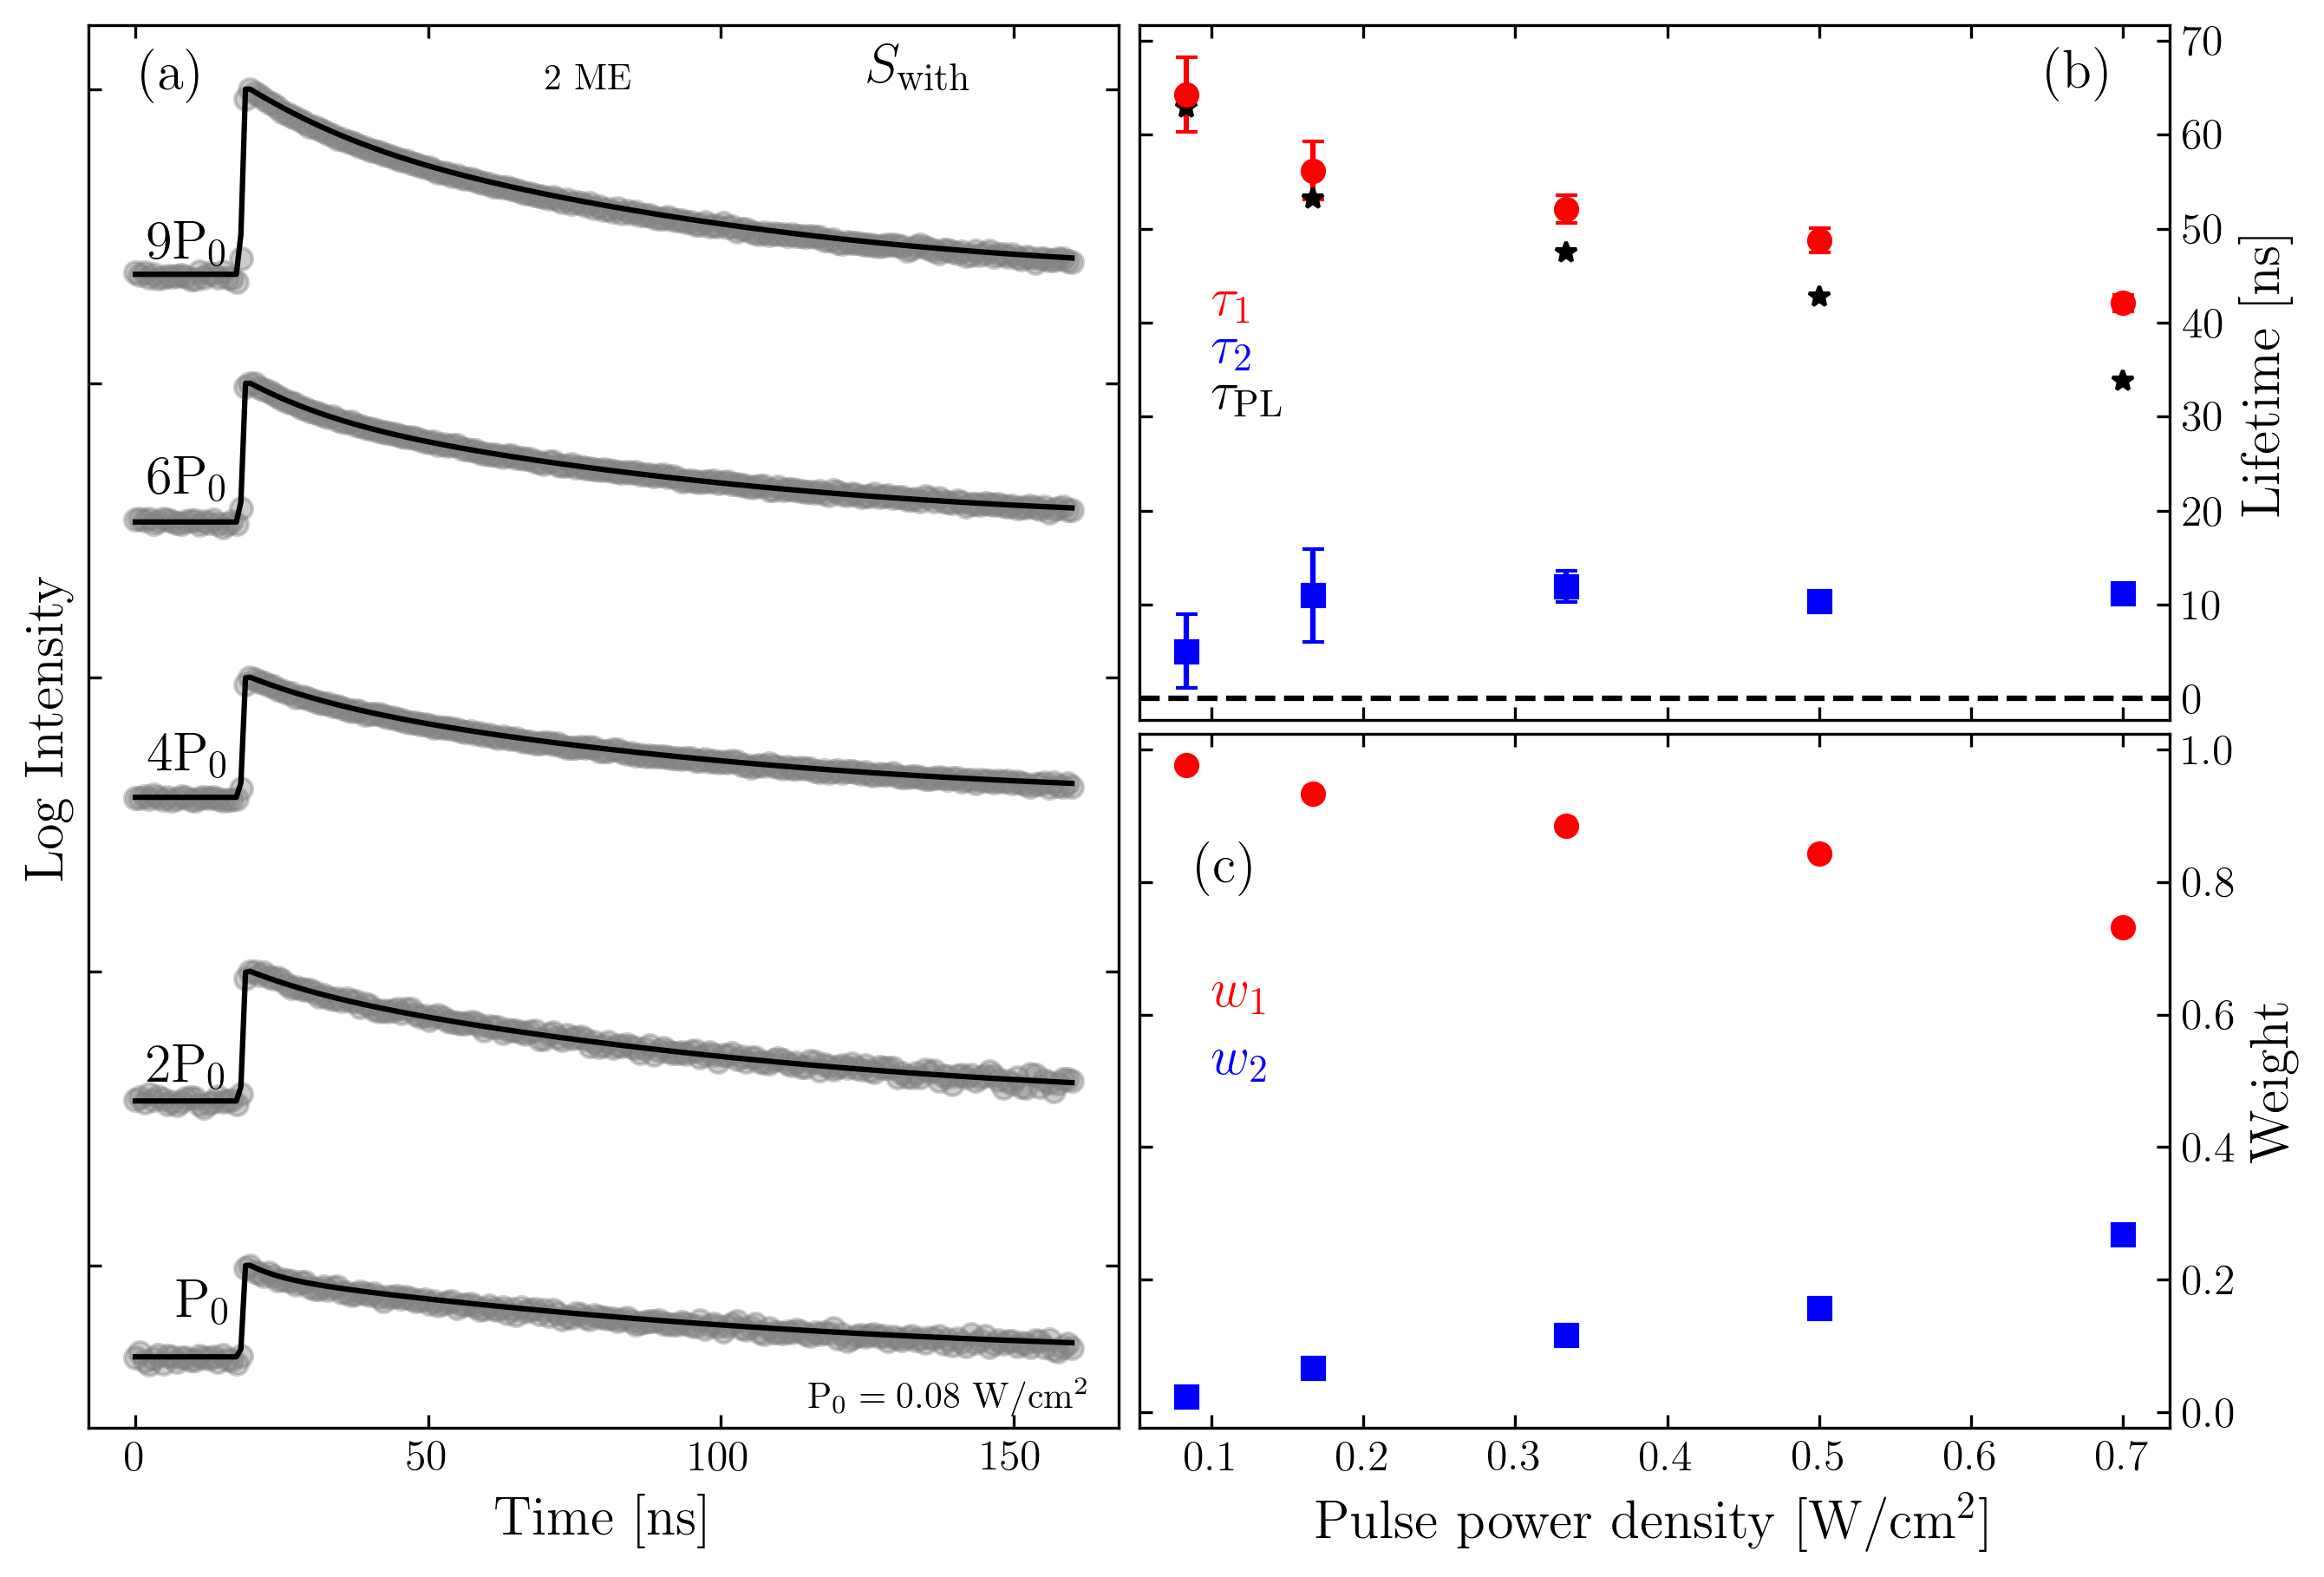
\includegraphics[width=1\linewidth]{/TRPL/intensity/12040_TRPL_Tfw0_int}
	\caption{(a) Experimental TRPL measured at 15~K as a function of excitation density (grey circles) and its deconvolution by 2ME model (solid lines) at the maximum of band $M_1^\mathrm{w}$ for sample $S_\mathrm{with}$. (b) Fitted decay times $\tau_1$ (red circles), $\tau_2$ (blue squares) and characteristic time $\tau_\mathrm{PL}$ (black stars) as a function of excitation density. Appropriate weights are shown in panel (c).}
	\label{fig:TRPL_int_w}
\end{figure}
Other samples given in appendix~\ref{chapter:appendix_TRPL_int} show similar behaviour and with comparable $\tau_\mathrm{PL}$ at low excitation power. However, $\tau_\mathrm{PL}$ of samples with QDs is approximately twice as small, see Fig.~\ref{fig:TRPL_int_all}(b).

\newpage
\subsection{Temperature dependent TRPL}
TRPL variations with temperature are shown in Figs.~\ref{fig:TRPL_temp_wo}-\ref{fig:TRPL_temp_c} and are deconvoluted again by 2ME model. As it can be seen in Fig.~\ref{fig:TRPL_temp_w}, the resulting decay times of sample $S_\mathrm{with}$ increase up to the temperature of 30~K and then progressively reduce which is characteristic of the appearance of thermally activated scape paths~\citep{Manna_apl2012_TRPLtype2}. Contrary to sample $S_\mathrm{with}$, on $S_\mathrm{w/o}$ and $S_\mathrm{cap}$ the reduction of the decay times begins at the lowest temperatures without an increase at the beginning.
%
\begin{figure}
	\centering
	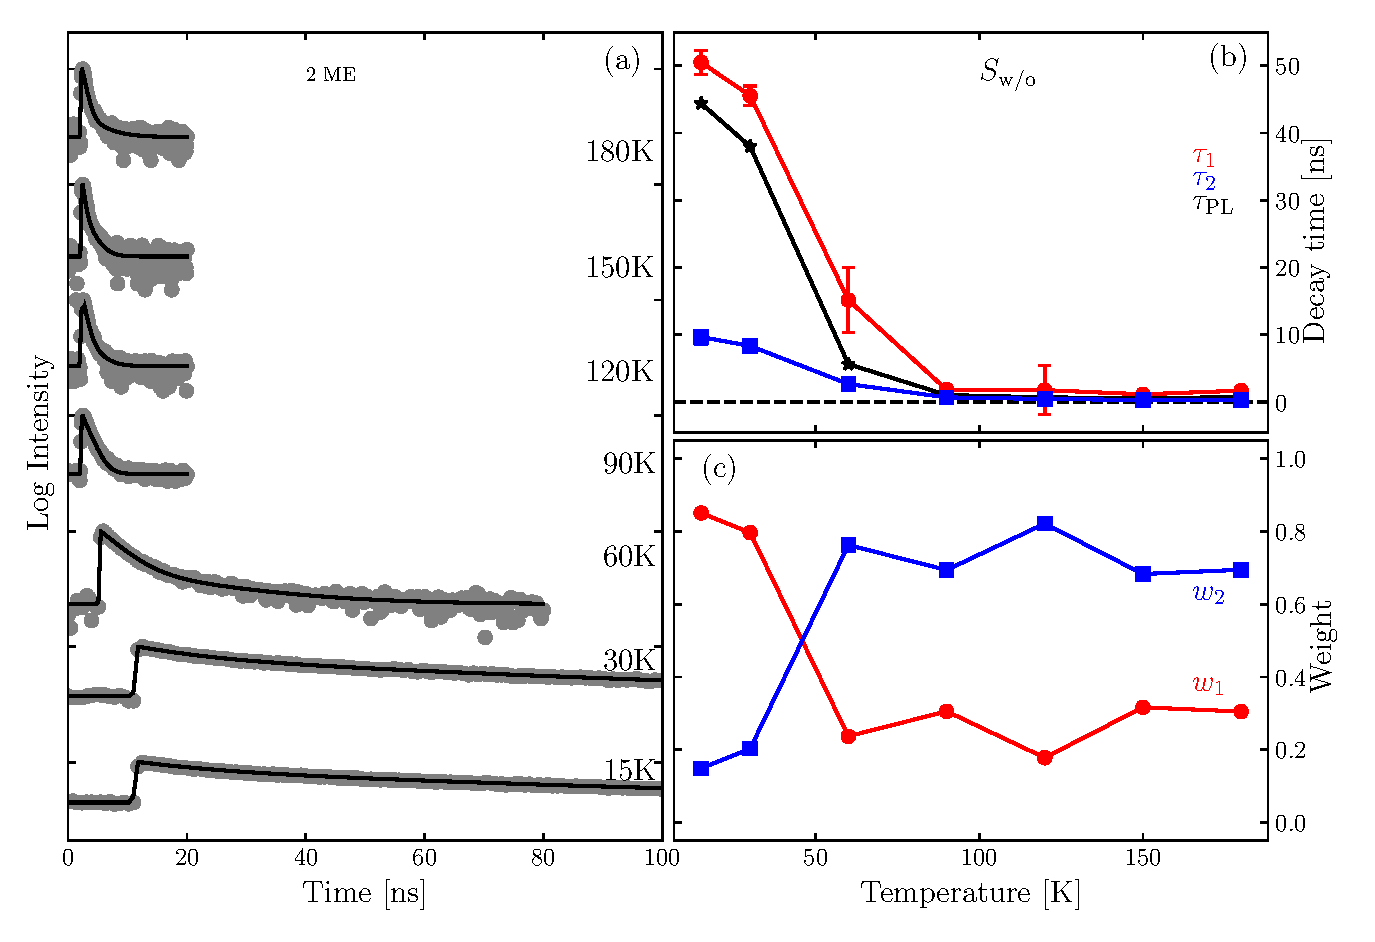
\includegraphics[width=0.9\linewidth]{/TRPL/temperature/12027_TRPL_max677_temp}
	\caption{(a) Experimental TRPL at pumping power of 0.3~W/cm$^2$ as a function of temperature (grey circles) and its deconvolution by 2ME model (solid black lines) at the maximum of PL signal in sample $S_\mathrm{w/o}$. (b) Deconvolved decay times ($\tau_1$: red circles; $\tau_2$: blue squares) and characteristic time $\tau_\mathrm{PL}$ (black stars) as a function of temperature. Corresponding weights are shown in panel (c).}
	\label{fig:TRPL_temp_wo}
\end{figure}
%
\begin{figure}
	\centering
	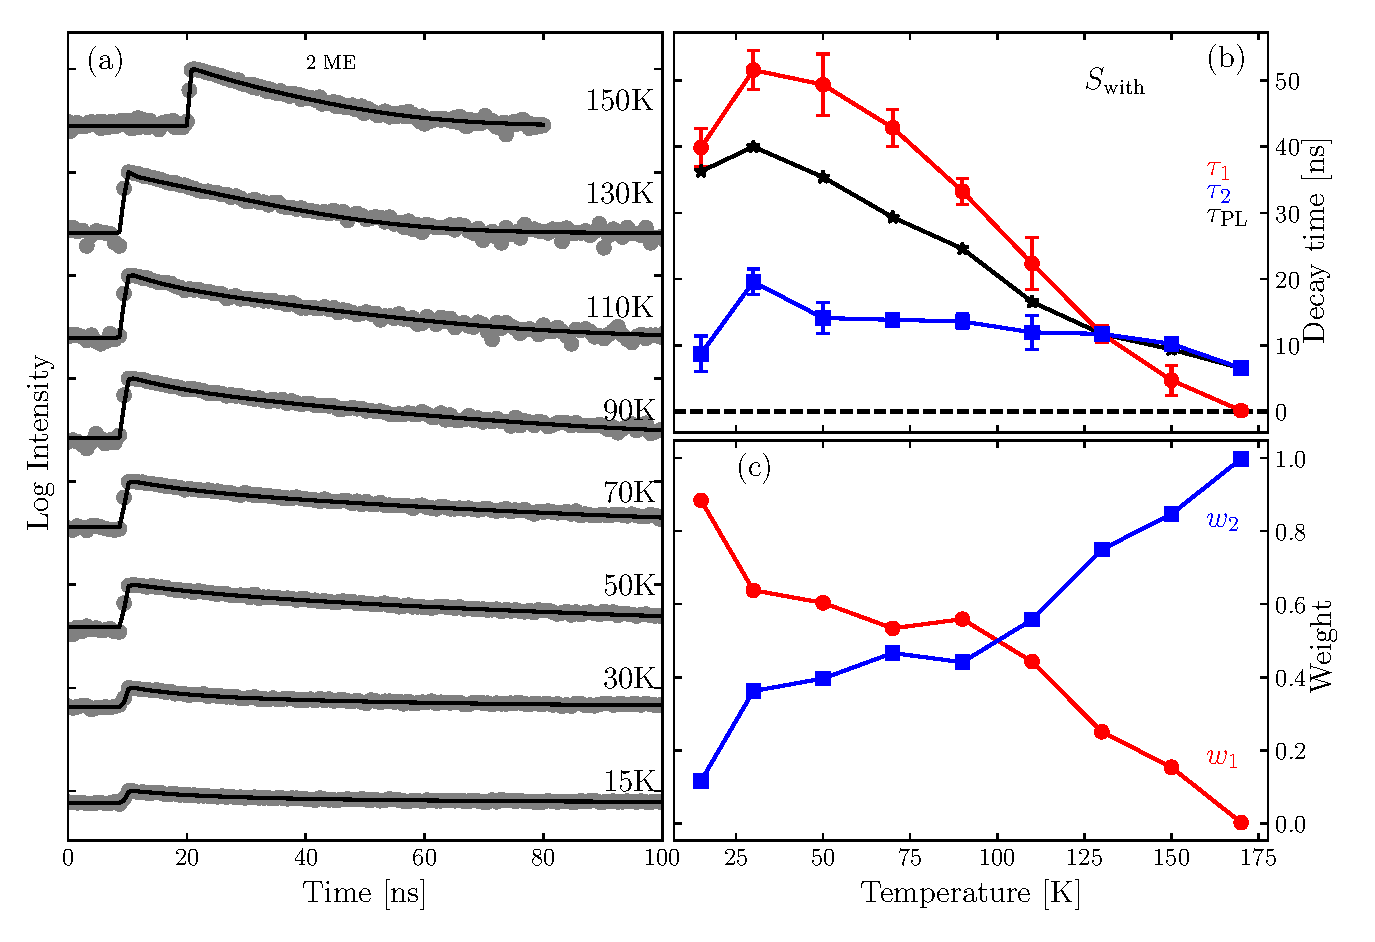
\includegraphics[width=0.9\linewidth]{/TRPL/temperature/12040_TRPL_700-710_temp}
	\caption{TRPL signal as a function of temperature at the maximum of PL in sample $S_\mathrm{with}$ similarly commented as in Fig.~\ref{fig:TRPL_temp_wo}.}
	\label{fig:TRPL_temp_w}
\end{figure}
%

If we assume similarly as in Ref.~\citep{t_alvarez} that at 15~K the only loss mechanism is radiative recombination, the radiative $\tau_\mathrm{R}$ and non-radiative $\tau_\mathrm{NR}$ decay times can be extracted from $\tau_\mathrm{PL}$ by
%
\begin{equation}
\tau_\mathrm{R}=\frac{I_0}{I_\mathrm{PL}(T)}\tau_\mathrm{PL} \label{eq:tau_R_fromPL}
\end{equation}
and
\begin{equation}
\frac{1}{\tau_\mathrm{PL}}=\frac{1}{\tau_\mathrm{R}} + \frac{1}{\tau_\mathrm{NR}}
\end{equation}
%
\begin{figure}
	\centering
	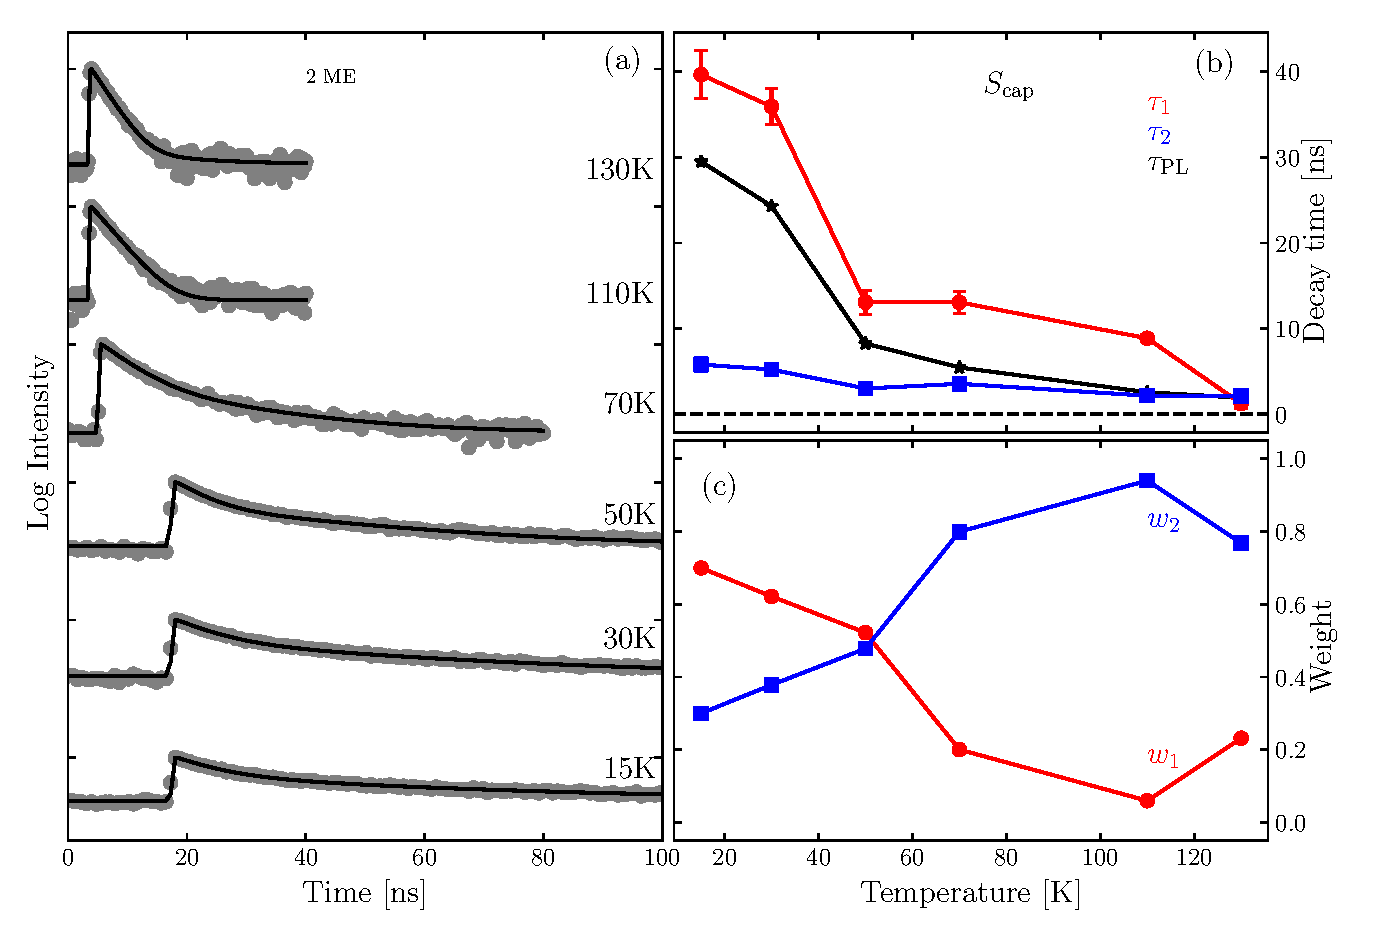
\includegraphics[width=0.9\linewidth]{/TRPL/temperature/12021_TRPL_690_temp}
	\caption{TRPL signal as a function of temperature at the maximum of PL in sample $S_\mathrm{cap}$ similarly commented as in Fig.~\ref{fig:TRPL_temp_wo}.}
	\label{fig:TRPL_temp_c}
\end{figure}
%

\noindent where $I_0$ and $I_\mathrm{PL}$ are the PL intensity at 15~K and that as a function of $T$, respectively. As can be seen in Fig.~\ref{fig:TRPL_temp_decon} $\tau_\mathrm{NR}$ decreases with temperature as is usually the case for thermally activated processes. Parameter $\tau_\mathrm{NR}$ can be fitted with two non-radiative processes 
%
\begin{equation}
\frac{1}{\tau_\mathrm{NR}}=\frac{1}{\tau_\mathrm{NR}^1}\exp{\left(\frac{-E_1}{k_\mathrm{B}T}\right)} + \frac{1}{\tau_\mathrm{NR}^2}\exp{\left(\frac{-E_2}{k_\mathrm{B}T}\right)} \label{eq:nonradiative}
\end{equation}
characterized by activation energies $E_1$ and $E_2$ and time constants $\tau_\mathrm{NR}^1$ and $\tau_\mathrm{NR}^2$, respectively.
Conversely, $\tau_\mathrm{R}$ increases exponentially with temperature
%
\begin{equation}
\tau_\mathrm{R} = \tau_\mathrm{R}^0 + \tau_\mathrm{R}^T \exp{\left(\frac{T}{T_C}\right)}, \label{eq:tau_R} 
\end{equation}
where $ \tau_\mathrm{R}^0$ ($ \tau_\mathrm{R}^T$) describes the temperature independent (dependent) part of the radiative decay and $T_C$ is the characteristic temperature corresponding to the energy of localized states. Inserting Eq.~(\ref{eq:tau_R_fromPL}) into Eq.~(\ref{eq:tau_R}) we can obtain an Arrhenius-like equation with an explicit dependence of the PL intensity on all the parameters derived from the TRPL analysis
%
\begin{equation}
I_\mathrm{PL}(T)=\frac{I_0}{1+\left[\tau_\mathrm{R}^0+\tau_\mathrm{R}^T\exp{\left(\frac{T}{T_C}\right)}\right] \times \left[\frac{1}{\tau_\mathrm{NR}^1}\exp{\left(\frac{-E_1}{k_\mathrm{B}T}\right)} + \frac{1}{\tau_\mathrm{NR}^2}\exp{\left(\frac{-E_2}{k_\mathrm{B}T}\right)}\right]}. \label{eq:TRPL_Arhenius}
\end{equation}
%
\begin{figure}
	\centering
	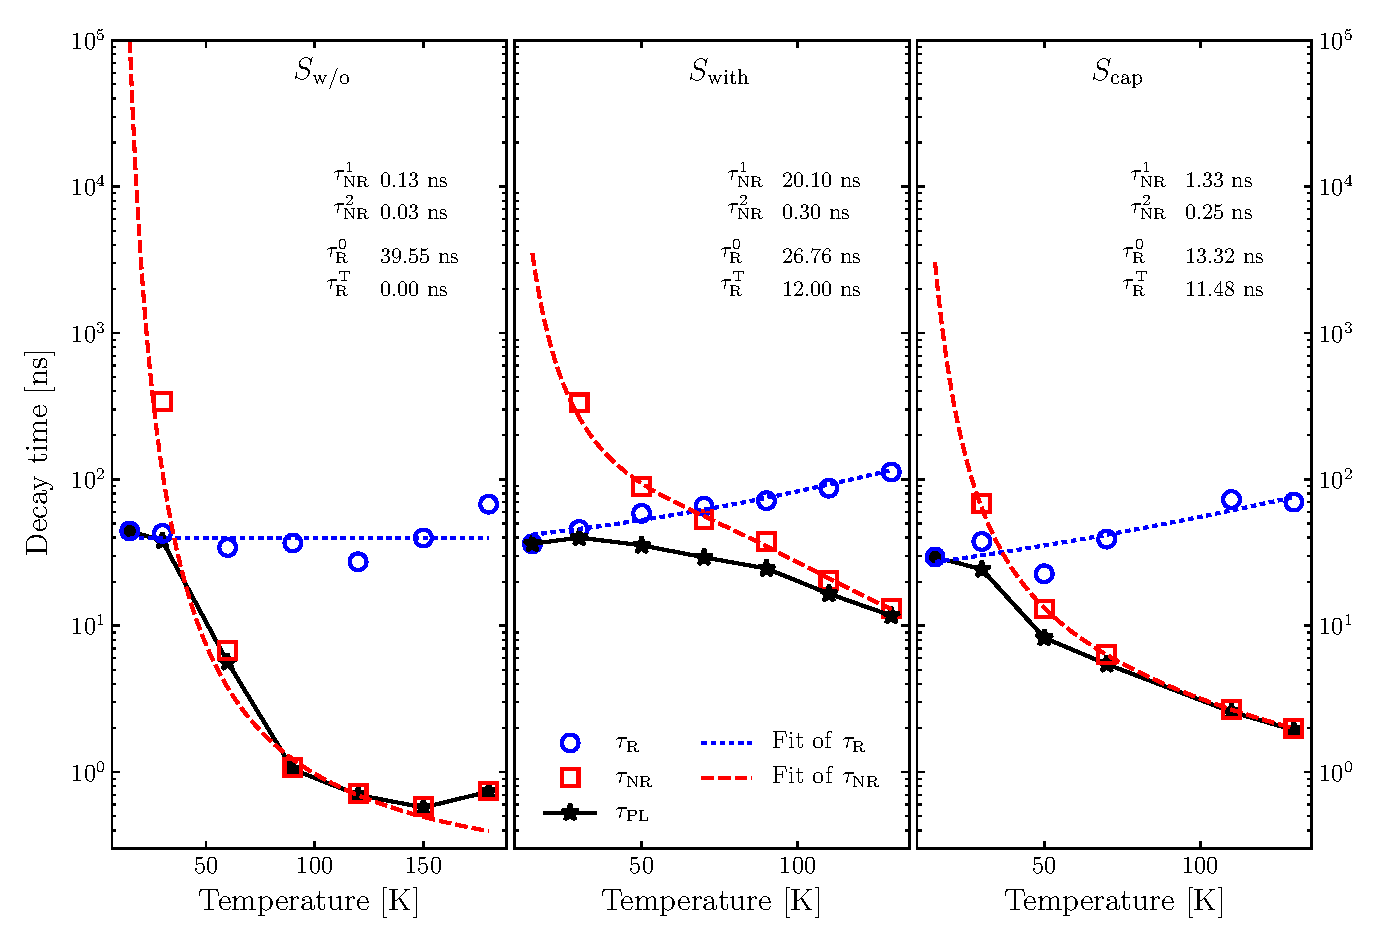
\includegraphics[width=1\linewidth]{/TRPL/temperature/decay_dekonvolution_all}
	\caption{Characteristic PL decay time $\tau_\mathrm{PL}$ as a function of temperature with the radiative and non-radiative components for all our samples. The radiative and non-radiative component are fitted by Eq.~(\ref{eq:tau_R}) and Eq.~(\ref{eq:nonradiative}), respectively.}
	\label{fig:TRPL_temp_decon}
\end{figure}

As it can be seen in Fig.~\ref{fig:Arrhenius_PLandTRPL}, this formula is equally good in reproducing experimental data as~Eq.~(\ref{eq:Arhenius}). 


\newpage

We now discuss the numerical results obtained in this analysis that are summarized in Tab.~\ref{tab:TRPL_params}. As can be seen in Fig.~\ref{fig:TRPL_temp_decon} the radiative decay time of $S_\mathrm{w/o}$ does not depend on temperature and is described only by $\tau_\mathrm{R}^0=39.6$~ns. On the contrary, the radiative decay time of samples with QDs exponentially grows with temperature and is proportional to similar value, i.~e., $\tau_\mathrm{R}^T=12.0$~ns for $S_\mathrm{with}$ and $11.5$~ns for $S_\mathrm{cap}$, respectively. 
The non-radiative process with smaller activation energy ($E_1$ between 6 and 18~meV) is probably associated with trapping of carriers by impurities or defects in the vicinity of QDs, as it has been also before for InAs/InP quantum wires~\citep{Alen_apl2011}. The other process is characterized by faster time constant $\tau_\mathrm{NR}^2$ ($\tau_\mathrm{NR}^1/\tau_\mathrm{NR}^2>5$) is close to the thermally activated capture of excitions by nonradiative defects in GaAs layer~\citep{Seravallo_apl2005,Kohki_apl1997}. 

The values obtained by fitting the dependencies by model in Eq.~(\ref{eq:TRPL_Arhenius}) are summarized in Tab.~\ref{tab:TRPL_params} and are comparable with parameters gained from the temperature dependence PL data shown in Sec.~\ref{Sec:temp_PL_TU}, which are equally well reproduced by Eq.~\ref{eq:Arhenius}, see the parameters resume in Tab.~\ref{tab:Arhenius}.

The previous temperature dependent TRPL and PL analysis of the samples allow us to draw simple scheme of the time evolution of the levels involved in the exciton dynamics, namely that of the recombining level \textbf{F} and three trap levels \textbf{N$_i$}, see Fig.~\ref{fig:Arrhenius_PLandTRPL}.
\begin{table}
	\centering
	\caption{Summary of the TRPL Arrhenius-like fits. The displayed values are obtained with accuracy better than $10^{-3}\%$.}
	\begin{tabularx}{0.9\textwidth}{cCCccccc}
		\toprule
		
		 & $E_1$ [meV]& $\tau_\mathrm{NR}^1$ [ns]& $E_2$ [meV]& $\tau_\mathrm{NR}^2$ [ns] & $\tau_\mathrm{R}^0$ [ns]& $\tau_\mathrm{R}^T$ [ns]& $T_C$ [K]\\ 	
		\midrule
		\midrule
		$S_\mathrm{w/o}$& 17.5&0.13&294.3 & 0.03& 39.55&0.00&8825.0\\
		$S_\mathrm{with}$&6.7 & 20.10& 47.2&0.30& 26.76&12.00&64.9\\
		$S_\mathrm{cap}$& 10.0&1.33&33.8 & 0.25& 13.32&11.48&76.9\\
		
		\bottomrule
	\end{tabularx}\label{tab:TRPL_params}
\end{table}



\begin{figure}
	\centering
	\includegraphics[width=0.9\linewidth]{/TRPL/temperature/models} %Arrhenius_PLandTRPL_all}
	\caption{The left panels (a)-(c) compare the integrated PL intensity and the corresponding fit for all our samples of the measurements performed with a CW (circles) and a pulsed (squares) laser. The right panels show levels involved in the exciton dynamics in our samples. The letters \textbf{0} and \textbf{F} in these sketches represent the vacuum end exciton state, respectively, \textbf{N$_i$} are three trap levels.}
	\label{fig:Arrhenius_PLandTRPL}
\end{figure}
\newpage 
%\input{Chapter4_SciRep/dip_ch4_scirep.tex}

%%% -------------------------------------------------------------
\appendix
\chapter{More information from TEM and EDX experiments}
\label{chapter:appendix_TEM}
We measured TEM together with EDX to get information on the chemical composition of sample S$_\mathrm{cap}$. The results shown in Fig.~\ref{fig:TEM_app} confirm the constituents given in Fig.~\ref{fig:TUstructure}.


\begin{figure}
	\centering
	\includegraphics[width=0.77\linewidth]{/TEM/TEM_appendix/TEM_12040}
	\caption{(a) TEM image measured under bright field conditions using the (200) reflection perpendicular to the growth direction. (b) EDX map in Al which is present only in Al$_{0.4}$GaP layer.}
	\label{fig:TEM_app}
\end{figure}

The emission EDX spectrum (Fig.~\ref{fig:EDX}) shows all elements present in S$_\mathrm{cap}$ sample, i.~e., Ga, P, In, As, Sb, Al; oxygen is detected due to degradation of the sample by oxidation processes; Co, Fe and Zr are typical compounds used in TEM objectives. In Fig.~\ref{fig:concentration_appendix} the distribution of the concentration in the vertical cut is shown, Al$_{0.4}$GaP layer and QD areas are located between 250 and 280$\,$nm and around 80$\,$nm, respectively.
\begin{figure}
	\centering
	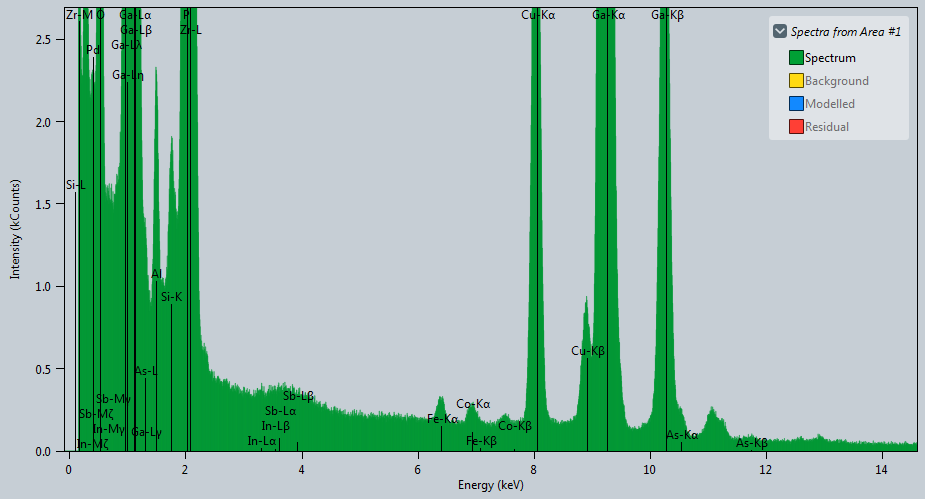
\includegraphics[width=0.77\linewidth]{/TEM/TEM_appendix/EDX}
	\caption{EDX spectrum measured on S$_\mathrm{cap}$.}
	\label{fig:EDX}
\end{figure}


\begin{figure}
	\centering
	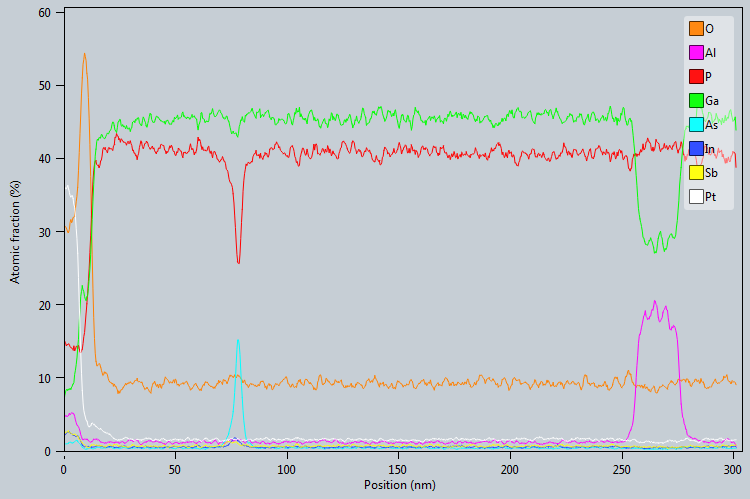
\includegraphics[width=0.77\linewidth]{/TEM/TEM_appendix/concentration}
	\caption{Atomic fraction as a function of position in the vertical cut (the zero position is associated with the surface of the sample).}
	\label{fig:concentration_appendix}
\end{figure}

\newpage 
\chapter{Time-resolved photoluminiscence of In$_{1-x}$Ga$_{x}$As$_y$Sb$_{1-y}$/GaAs/GaP QDs samples}

\section{Excitation density TRPL}
\label{chapter:appendix_TRPL_int}
\begin{figure}
	\centering
	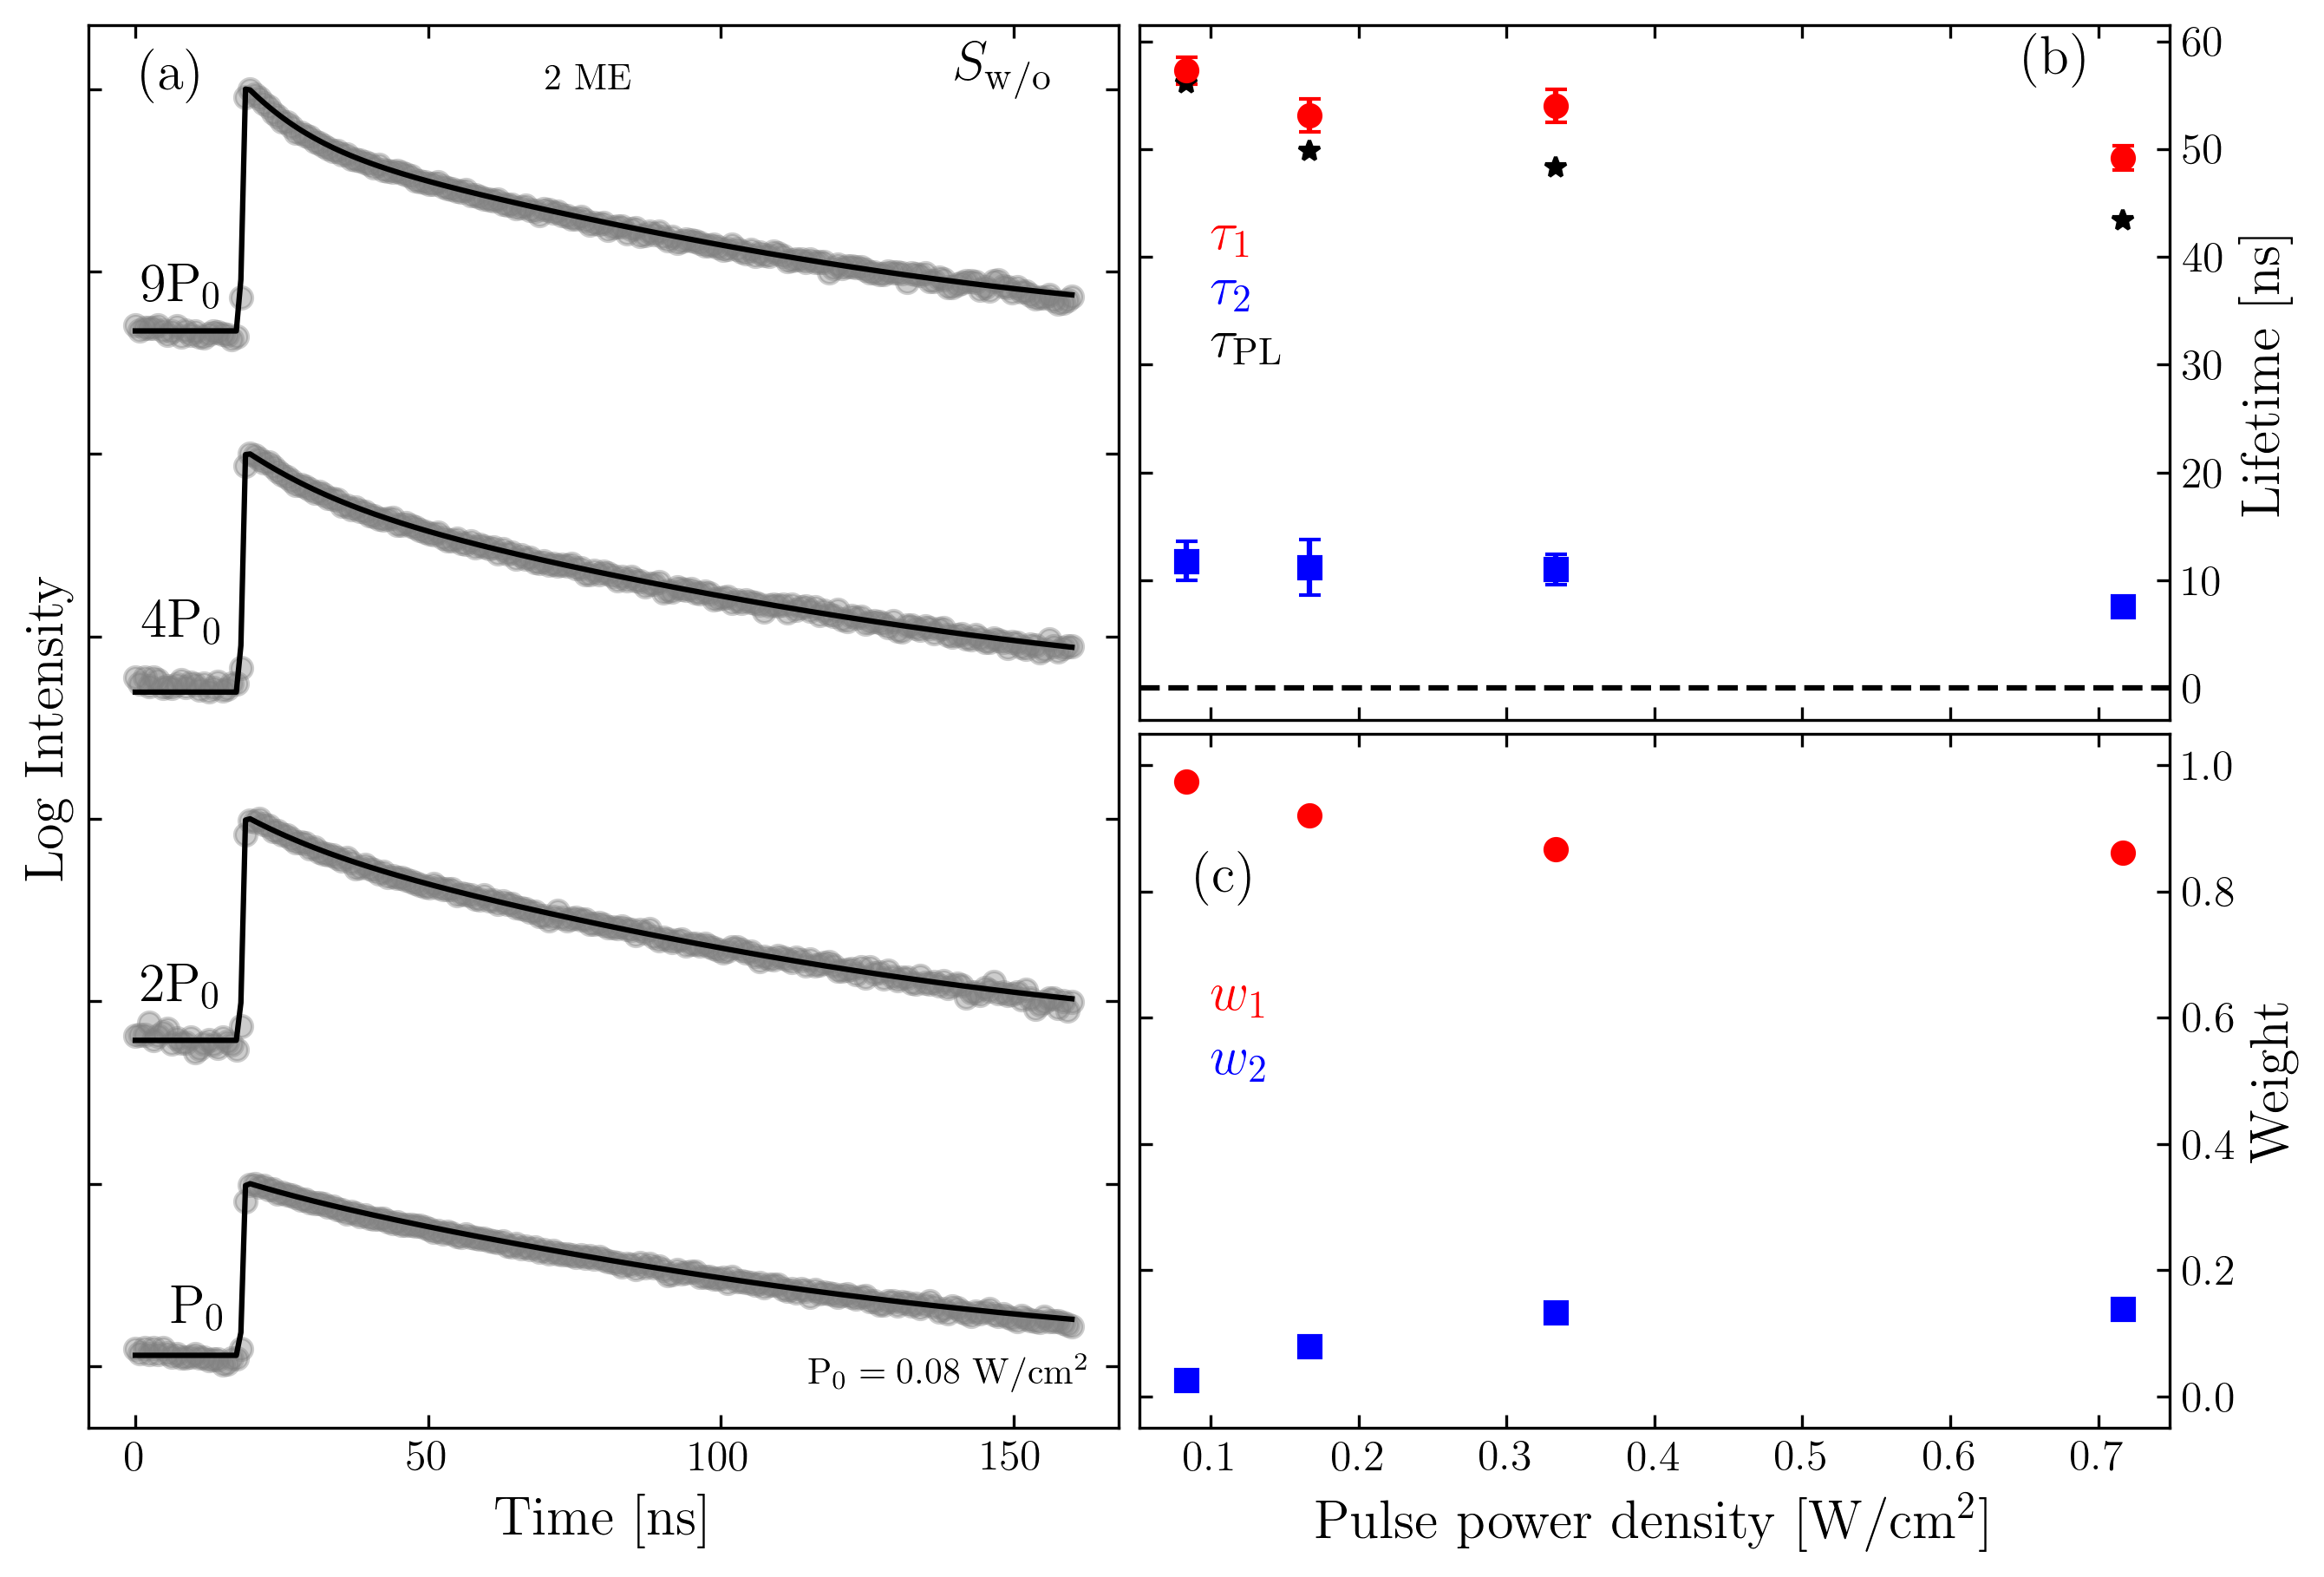
\includegraphics[width=0.9\linewidth]{/TRPL/intensity/12027_TRPL_max677_int}
	\caption{(a) TRPL measured at 15~K as a function of excitation density (grey circles) and its deconvolution by 2~ME model (solid lines) at the maximum of band $M_1^\mathrm{w/o}$ in the sample $S_\mathrm{w/o}$. (b) Fitted decay times $\tau_1$ (red circles), $\tau_2$ (blue squares) and characteristic time $\tau_\mathrm{PL}$ (black stars) as a function of excitation density. Appropriate weights are visualized in panel (c).}
	\label{fig:TRPL_int_wo}
\end{figure}


\begin{figure}
	\centering
	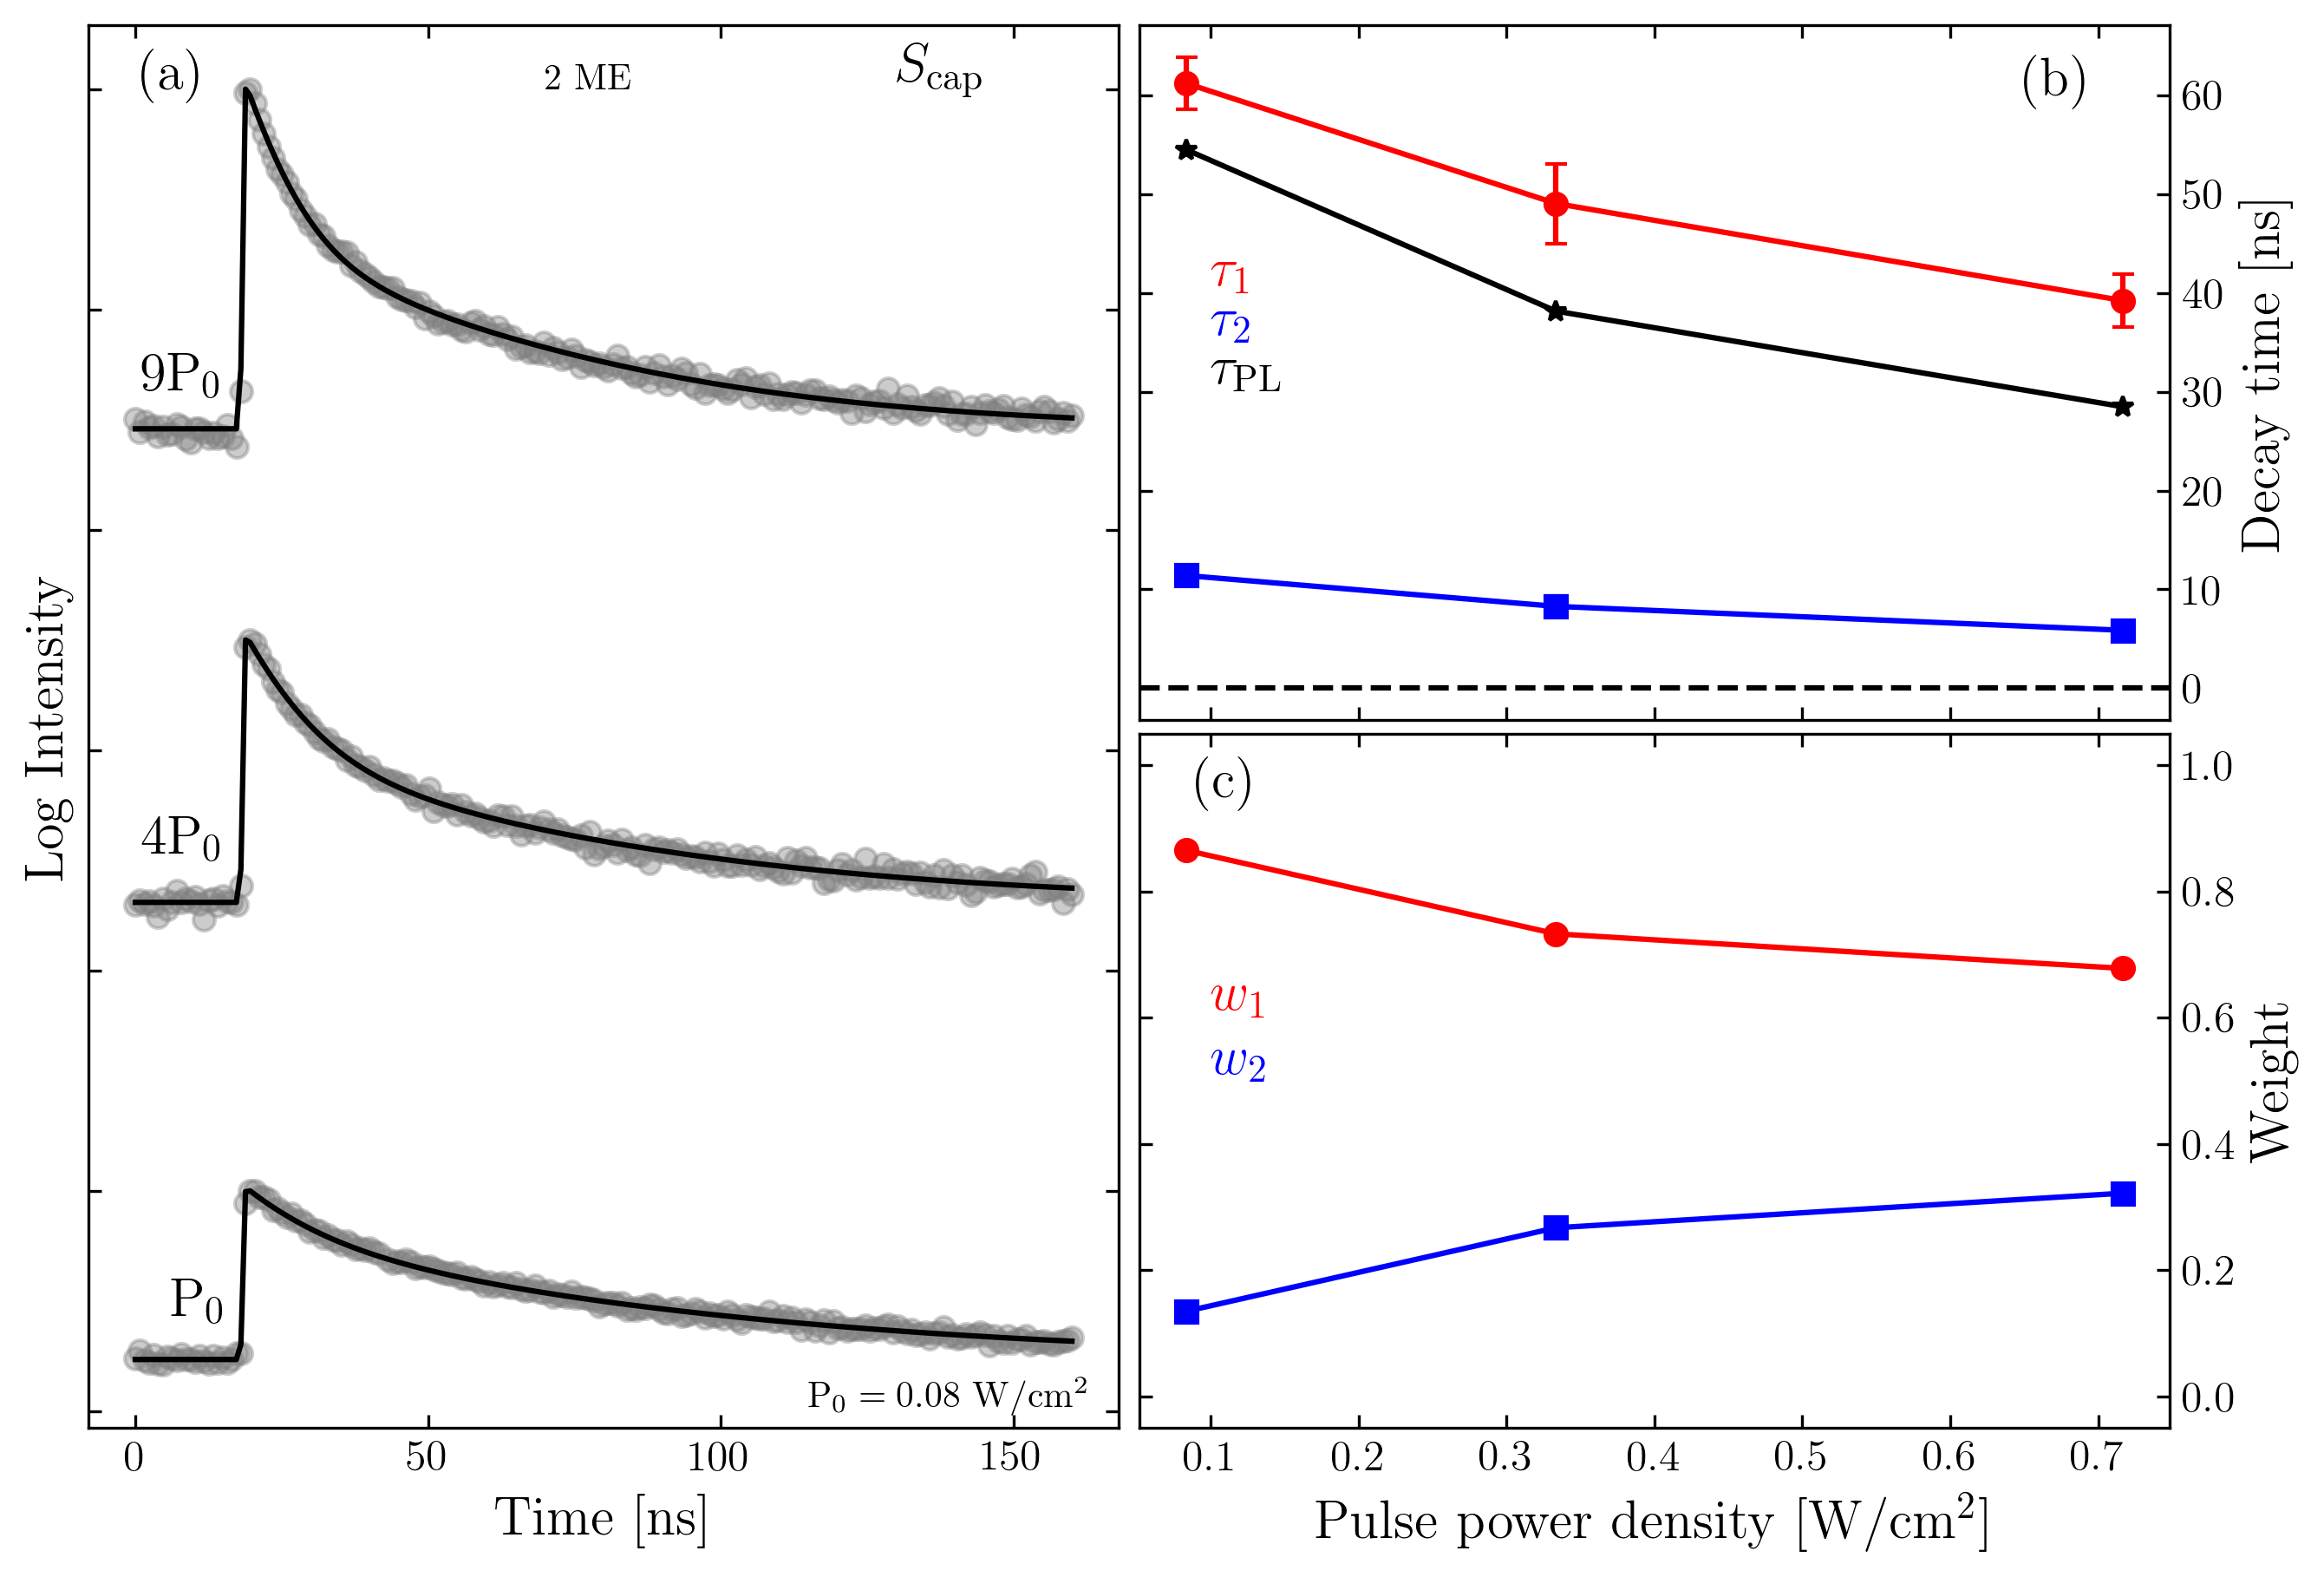
\includegraphics[width=0.9\linewidth]{/TRPL/intensity/12021_TRPL_max710_int}
	\caption{TRPL spectra of the maximum of band $M_1^\mathrm{c}$ in sample $S_\mathrm{cap}$. The results are given in the same nomenclature as in Fig.~\ref{fig:TRPL_temp_wo}.}
	\label{fig:TRPL_int_c}
\end{figure}
\newpage 
%\chapter{Derivation of the relation between in-plane stress in principal and Cartesian coordinates}
\label{app:principal_stress}

Any in-plane stress configuration can be described by three independent components of stress tensor ($\sigma_{xx}$, $\sigma_{yy}$, and $\sigma_{xy}$) or, equivalently, by two principal stresses $\sigma_\mathrm{max}$ and $\sigma_\mathrm{min}$ applied at an angle $\alpha$ with respect to the crystal axis. We now introduce the connection between the Cartesian and principal components.

We first rotate the basis of the stress components $\sigma_{xx}$, $\sigma_{yy}$ and $\sigma_{xy}$ by an angle $\theta$ to obtain components $\sigma_{xx}'$, $\sigma_{yy}'$ and $\sigma_{xy}'$ in the rotated basis which are related to the previous ones by
%
\begin{align}
\sigma_{xx}' &= \sigma_{xx}\cos^2{\theta}+\sigma_{yy}\sin^2{\theta}+2\sigma_{xy}\sin{\theta}\cos{\theta} , \\
\sigma_{yy}' &=\sigma_{xx}\sin^2{\theta}+\sigma_{yy}\cos^2{\theta}-2\sigma_{xy}\sin{\theta}\cos{\theta}, \\
\sigma_{xy}' &=\left(\sigma_{xx}-\sigma_{yy}\right)\sin{\theta}\cos{\theta}+\sigma_{xy}\left(\cos^2{\theta}-\sin^2{\theta}\right).
\end{align}
%
%
%
%
Principal stress orientation can be then computed by setting $\sigma_{xy}'=0$ in the last equation and solving
%
%
\begin{equation}
\sigma_{xx}\sin^2{\theta}+\sigma_{yy}\cos^2{\theta}-2\sigma_{xy}\sin{\theta}\cos{\theta}=0,
\end{equation}
%
%
for $\theta$. The result is the equation giving the principal stress angle which we denote $\alpha$
%
%
\begin{equation}
\tan{2\alpha}=\frac{2\sigma_{xy}}{\sigma_{xx}-\sigma_{yy}}\label{eq:principal_angle}.
\end{equation}
%
Inserting $\alpha$ back into the Eqs.~(1)--(3) we obtain the principal stress values $\sigma_\mathrm{max}$ and $\sigma_\mathrm{min}$
%
%
\begin{equation}
\sigma_\mathrm{max}, \sigma_\mathrm{min} = \frac{\sigma_{xx}+\sigma_{yy}}{2} \pm \sqrt{\left(\frac{\sigma_{xx}-\sigma_{yy}}{2}\right)^2+\sigma_{xy}^2}. \label{eq:princip_strain}
\end{equation}
%
%



We then express the sum and the difference of $\sigma_\mathrm{max}$ and $\sigma_\mathrm{min}$
%
\begin{align}
\sigma_{\mathrm{max}}+\sigma_{\mathrm{min}} &= \sigma_{xx}+\sigma_{yy}, \label{eq:plus}\\
\sigma_{\mathrm{max}}-\sigma_{\mathrm{min}} &= \sqrt{\left(\sigma_{xx}-\sigma_{yy}\right)^2+4\sigma_{xy}^2}.\label{eq:minus}
\end{align}
%
If we now combine equations (\ref{eq:princip_strain}) with (\ref{eq:minus}) we can write
%
%
\begin{equation}
\label{eq:nxyVSnprinc}
\sigma_{xy}=\frac{1}{2}\left(\sigma_{\mathrm{max}}-\sigma_{\mathrm{min}}\right)\sin{2\alpha}.
\end{equation}
%

\newpage 

%\chapter{Causality}

%\lipsum[1-2]

\backmatter

%%% BIBLIOGRAPHY
%%% -------------------------------------------------------------


%\bibliography{example2}
%\bibliographystyle{plainnat}
%\bibliographystyle{alpha}
\bibliographystyle{plainnat}
\bibliography{dip_ps_ref}

\end{document}